\documentclass[11pt]{book}

%%%% Fill out all these macros
\newcommand{\thesisTitle}{Data analysis tools for statistical non-experts}
\newcommand{\authorName}{Eunice Jun}
\newcommand{\advisor}{Jeffrey Heer}
\newcommand{\advisorTitle}{Jerre D. Noe Endowed Professor} % assistant, associate prof?
\newcommand{\advisorDepartment}{Paul G. Allen School of Computer Science \& Engineering}
% if you have two advisors, uncomment these two
\newcommand{\secondAdvisor}{Ren\'{e} Just}
\newcommand{\secondAdvisorTitle}{Associate Professor}
\newcommand{\secondAdvisorDepartment}{Paul G. Allen School of Computer Science \& Engineering}

\newcommand{\readingCommitteeOne}{Tyler H. McCormick}
\newcommand{\graduationYear}{2023}

%\usepackage{} -- add any other packages you want
%\usepackage{proceed2e}
\usepackage[hyphens]{url}
\usepackage{amsfonts}
\usepackage{multirow,tabularx}
\usepackage{listings}
\usepackage{makecell}
\usepackage[linesnumbered]{algorithm2e}
\usepackage{amssymb}
\usepackage{graphicx}
\usepackage{amsmath}
\usepackage{float}
\usepackage{fullpage}
\usepackage{mathrsfs}
\usepackage{subcaption}
\usepackage{hyperref}% http://ctan.org/pkg/hyperref
\hypersetup{%
  %colorlinks = true,
  linkcolor  = black
}
\usepackage{mdwlist}
\usepackage{xspace}
\usepackage{setspace}
\usepackage{times} % Set the typeface to Times Roman
\usepackage[scaled]{helvet} % ss
\usepackage{courier} % tt
\normalfont
\usepackage[T1]{fontenc}


%\usepackage[showframe=true]{geometry}
\usepackage{changepage}
\usepackage[labelfont=bf]{caption} % boldface caption title for floats
\usepackage[square]{natbib}
\usepackage{enumitem}
\usepackage{natbib}
\usepackage{array,multirow}
\usepackage{fixltx2e}
\usepackage{booktabs}
\usepackage{bbm}
\usepackage{soul}
\usepackage{relsize}
\usepackage{eso-pic}
\usepackage{xspace}
\usepackage{epsfig}
\usepackage{graphicx}
\usepackage{amsmath}
\usepackage{amssymb}
\usepackage{float}
\usepackage{multirow}
\usepackage{rotating}
\usepackage{balance}
\usepackage{wrapfig}
\usepackage{enumerate}
\usepackage{caption}
\usepackage{framed}
\usepackage{enumitem}
\usepackage{multirow}
\usepackage{graphicx}
\usepackage{color}
\usepackage{fixltx2e}
%\usepackage{tkz-graph}
\usepackage{caption}
\usepackage{subcaption}
\usepackage{tikz}
\usepackage{mathtools}
\usepackage{pifont}
\usepackage{scrextend}
\usepackage{sidecap}
\usepackage{graphicx}

\usepackage{todo}
\DeclareUnicodeCharacter{2212}{-}
\newcommand{\tquote}[1]{\emph{\textcolor{darkgray}{``#1''}}}
\newcommand{\tableLitSurveyCodes}{
\footnotesize
\setlength{\extrarowheight}{10pt} % Add extra space
    \begin{longtable}{>{\raggedright}p{0.16\linewidth} p{0.80\linewidth} p{0.04\linewidth}}
        % xsize
        \caption{The \codebook for analyzing the content of research publications. The rightmost column is the percentage of paragraphs tagged with the code.} \\ 
        % \vspace{-15pt}
        \setlength{\tabcolsep}{4pt}
        % \begin{tabular}
        % x\hline
        \textbf{Codes} & \textbf{Definitions and Examples} & \textbf{\%Freq.} \\
        \toprule 
            %%%%
            \multicolumn{2}{l}{\textbf{Research Goals}}
            & \\
            & & \\ % For formatting
            %%% 
            Question or statement of unknown & 
            Explicit, clear statement about an unknown phenomenon or an open-ended question \newline
            \tquote{However, the ontogeny of holistic recollection is uncharted.}~\cite{PS9}
            & 4.2 \\
            & & \\ % For formatting
            %%% 
            Predicted outcomes & 
            A clear conjecture of an outcome that does not specify a specific mathematical relationship \newline
            \tquote{We hypothesized that the outward current is mainly carried by FA anions...}~\cite{N2}
            & 6.8 \\
            & & \\ % For formatting
            %%% 
            Specific statistical expectation & 
            A conjecture specifying how observations will be related to one another mathematically/statistically \newline
            \tquote{If this dependency measure (data-independent model) was significantly greater than zero, this provided evidence for significant retrieval dependency...}~\cite{PS9}
            & 0.1 \\
            & & \\ % For formatting
            %%% 
            Specific objectives & 
            Statements about reaching objectives \newline
            \tquote{To assess the potential clinical relevance of the neo-development of a neuronal network in prostate cancer, DCX+ cells were quantified in benign prostate hyperplasia...}~\cite{N9}
            & 2.6 \\
            & & \\ % For formatting
            %%% 
            Examination of associations & 
            A statement about examining a relationship between two or more concepts \newline
            \tquote{We next examine whether proxies for these factors appear to affect the transactions costs in the secondary market for private equity stakes.}~\cite{JFE2}
            & 3.8 \\
            & & \\ % For formatting
            %%% 
            \midrule
            %%%%
            \multicolumn{2}{l}{\textbf{Data Sample Information}} \\
            & & \\ % For formatting
            %%% 
            Study design and protocol & 
            Information about the procedures used or prototypes developed to collect the data for analysis, such as any assays or experimental designs, including any limitations (e.g, conditions/randomization, interventions, treatments) \newline
            \tquote{Before the experiment, we introduced the working principle of HandSee. Then we tested the techniques one by one. For each technique, we first demonstrated our interaction technique. After...}~\cite{CHI3}
            & 20.8 \\
            & & \\ % For formatting
            %%% 
            Initial data sourcing & 
            Information about the source, size, and characteristics of the data sample that was collected or analyzed \newline
            \tquote{A total of 32 four-year-old children (15 female; age: M = 52.05 months, SD = 3.37) and 30 six-year-old children (17 female; age: M = 76.37 months; SD = 2.16) from the Philadelphia area participated in the study...} ~\cite{PS9}
            & 9.8 \\
            & & \\ % For formatting
            %%% 
            Data filtering/sampling & 
            Any criteria, procedures, and decisions to filter, remove, combine, and split data for data quality, sub-analyses, or robustness (e.g., sampling from existing datasets, removing outliers, etc.) \newline
            \tquote{As for the US data, we restrict our attention to sectors with ten or more firms. } ~\cite{JFE9}
            & 6.4 \\
            & & \\ % For formatting
            %%% 
            Details about data used for analysis & 
            Any summary statistics (e.g., mean, standard deviation, distribution, etc.) and other information describing the final data sample used for statistical analysis \newline
            \tquote{All subjects' mean values were within 2.5 standard deviations from the group mean; therefore, they were all included in the following analyses.} ~\cite{PS7}
            & 2.9 \\
            & & \\ % For formatting
            %%%
            \midrule
            %%%%
            \multicolumn{2}{l}{\textbf{Statistical Analysis}} \\
            & & \\ % For formatting
            %%% 
            Proxy & 
            Any information about how concepts are measured, including any limitations, etc.; Can be established or new ways of measuring a construct \newline
            \tquote{Our definition of a price run-up is based on the industry value-weighted return.} ~\cite{JFE9}
            & 12.3 \\
            & & \\ % For formatting
            %%% 
            Equation & 
            Any mathematical equation, using symbols or sentences \newline
            \tquote{The absolute number of cells was calculated as ((number of Lin−eYFP+ cells acquired $×$ cellularity of the organ)/number of live single cells acquired).} ~\cite{N9}
            & 2.4 \\
            & & \\ % For formatting
            %%% 
            Statistical specification & 
            Describing a statistical model (e.g., linear regression), test (e.g. Student's t-test), or other procedure (e.g., contingency table) for analyzing the data \newline
            \tquote{Frequentist null-hypothesis significance testing was complemented with Bayesian hypothesis testing, which quantified the evidence for the presence or absence of effects...} ~\cite{PS0}
            & 18.7 \\
            & & \\ % For formatting
            %%% 
            \midrule
            %%%%
            \multicolumn{2}{l}{\textbf{Results}} \\
            & & \\ % For formatting
            %%% 
            Statistical results & 
            Reporting the findings (not usage) of statistical analyses or models, refer to specific quantified metrics (e.g., ratio, coefficient, correlation, etc.) with specific values (e.g., numbers) or aspects of values (e.g., positive estimate, positive relationship) \newline
            \tquote{In all experiments, when the entire sample size (N 24) was included in the analyses, the main findings in each experiment remained significant for all color-memory estimates (for paired comparisons, all ts > 2.74, ps  .012, and BF10s = 4.32; for three-group comparisons, all Fs > 7.07, ps  .0021, and BF10s = 16.64).}~\cite{PS0}
            & 10.7 \\
            & & \\ % For formatting
            %%% 
            Interpreted results & 
            What the statistical results mean conceptually \newline
            \tquote{This result supports the notion that the economies of scale...can induce larger firms to hedge more extensively.} ~\cite{JFE1}
            & 30.9 \\
            & & \\ % For formatting
            %%% 
            Causal model & 
            A causal model or mechanism (with a clear cause and effect) supported by the data and statistical analysis results \newline
            \tquote{Here we show that GUN1 interacts with MORF2/RIP2 (herein only the name MORF2 will be used) to affect the efficiency of editing for multiple sites in plastid RNAs during...} ~\cite{PNAS0}
            & 0.2 \\
            & & \\ % For formatting
            %%% 
            Results from other non-statistical methods & 
            Any results derived from methods other than statistics; could be from qualitative, observational, or visual analyses \newline
            \tquote{Feeling deceived by Yelp, users (n=14) demanded a “full disclosure” (O120) of the algorithm's presence through the interface design by putting the filtered reviews in “PLAIN SIGHT” (O120)...} ~\cite{CHI4}
            & 7.3 \\
            & & \\ % For formatting
            %%% 
            Other outcomes & 
            Implications for what the results could lead to, future research \newline
            \tquote{Lastly, our work might fuel a new investigation into the uncanny valley of haptics [4].} ~\cite{CHI0}
            & 1.6 \\
            & & \\ % For formatting
            %%% 
            Limitations & 
            Any caveats or limitations about the statistical results \newline
            \tquote{We acknowledge that a limitation of the present study is that the sample size may not be considered particularly large.} ~\cite{PS1}
            & 1.1 \\
            & & \\ % For formatting
            %%% 
            \midrule
            %%%%
            \multicolumn{2}{l}{\textbf{Computation}} \\
            & & \\ % For formatting
            %%% 
            Software & 
            Any mention of software used for data analysis \newline
            \tquote{We calculated BFs using the BayesFactor package...for the R software environment...} ~\cite{PS0}
            & 2.9 \\
            & & \\ % For formatting
            %%% 
            Computational details & 
            Any details about parameters or other settings used for data analysis \newline
            \tquote{For mean comparisons, we used the t-test BF function with default settings (medium prior scale).} ~\cite{PS0}
            & 1.4 \\
            %%% 
        %     \midrule
            %%%%
            %%% 
        \bottomrule
        % \end{tabular}
        %\vspace{1pt}
        % \footnotesize
        \label{table:litSurveyCodeBook}
        \end{longtable}  
        \normalsize  
}

\newcommand{\tableCHIContribs}{
\setlength{\extrarowheight}{10pt} % Add extra space
\begin{longtable}{>{\raggedright}p{0.23\textwidth} p{0.4\textwidth}p{0.06\textwidth}p{0.06\textwidth}p{0.09\textwidth}p{0.06\textwidth}}
        % \centering
        % \footnotesize
        \caption{Summary of CHI papers in our dataset.} \\
        % \vspace{-15pt}
        \setlength{\tabcolsep}{4pt}
        % \begin{tabular}{>{\raggedright}p{0.31\linewidth} p{0.42\linewidth}p{0.06\linewidth}p{0.06\linewidth}p{0.09\linewidth}p{0.06\linewidth}}
        % \hline
        \textbf{Title} & \textbf{Short summary} & \textbf{Method} & \textbf{System} & \textbf{Empirical} & \textbf{Other} \\
        \toprule 
        %%%%
        \multicolumn{2}{l}{\textbf{ACM Conference on Human Factors in Computing Systems (CHI).}}
        & \\
        %%% 
        \midrule
        %%%%
        Detecting Visuo-Haptic Mismatches in Virtual Reality using the Prediction Error Negativity of Event-Related Brain Potentials~\cite{CHI0} & 
        The authors develop a new, more objective metric for haptic immersion. Through a user study, they find that the new metric is able to detect visuo-haptic mismatches in VR. & 
        \yes & 
        \no & 
        \no &
        \no \\
        & & & & & \\ % For formatting
        Engaging High School Students in Cameroon with Exam Practice Quizzes via SMS and WhatsApp~\cite{CHI1} & 
        The researchers provide study support through quiz questions delivered through SMS or WhatsApp. The researchers observe differences in participation during a three-week deployment. & 
        \no & 
        \no & 
        \yes &
        \no \\
        & & & & & \\ % For formatting
        Springlets: Expressive, Flexible and Silent On-Skin Tactile Interfaces~\cite{CHI2} & 
        Springlets is a mechano-tactile interface for skin. The authors discuss its design, fabrication, user perceptions, and possible applications. & 
        \no & 
        \yes & 
        \no &
        \no \\
        & & & & & \\ % For formatting
        HandSee: Enabling Full Hand Interaction on Smartphones with Front Camera-based Stereo Vision~\cite{CHI3} & 
        The authors are able to detect a phone user's gripping and touching interactions by using a mirror on the front camera to obtain stereo vision. & 
        \yes & 
        \yes & 
        \no &
        \yes \\
        & & & & & \\ % For formatting
        User Attitudes towards Algorithmic Opacity and Transparency in Online Reviewing Platforms~\cite{CHI4} & 
        The authors ask three research questions around how Yelp users view algorithmic control/intervention on the platform and how increasing their awareness of it through a system changes their perspectives and opinions about it. The authors find that individuals that are more invested in Yelp as reviewers are more likely to defend the platform's algorithms. & 
        \no & 
        \no & 
        \yes &
        \no \\
        & & & & & \\ % For formatting
        Slow Robots for Unobtrusive Posture Correction~\cite{CHI5} & 
        The authors develop and evaluate a system for automatically correcting user posture. The authors conduct two empirical studies, one formative and one evaluation. The formative study identifies end user perception of moving screens. The evaluation study evaluates user experience and how often users corrected their posture. The authors use mixed methods, both quantitative and qualitative/observational in their studies. & 
        \no & 
        \yes & 
        \no &
        \no \\
        & & & & & \\ % For formatting
        May AI? Design Ideation with Cooperative Contextual Bandits~\cite{CHI6} & 
        The authors develop a new technique and system for co-creation with an AI. They evaluate the effects of the AI on a series of task and creativity measures. They find that the AI is helpful in some dimensions. & 
        \no & 
        \yes & 
        \no &
        \no \\
        & & & & & \\ % For formatting
        The Effects of Interruption Timings on Autonomous Height-Adjustable Desks that Respond to Task Changes~\cite{CHI7} & 
        The authors investigate the most opportune time to adjust desks for improved ergonomics while minimizing interruption and annoyance/negative experiences during tasks. The authors find that changing desk height during task transition periods are the least disruptive, but end-users are dubious/have less trust in the automated adjustments. On the other hand, adjusting desk height after end-users have initiated a new task/changed tasks causes increased disruption but also increased trust in the automated desk. & 
        \no & 
        \no & 
        \yes &
        \no \\
        & & & & & \\ % For formatting
        Caring for Vincent: A Chatbot for Self-compassion~\cite{CHI8} & 
        The authors design a chatbot and then see how taking care of or being taken by the chatbot affects self-compassion. The authors test this hypothesis quantitatively and then follow-up with additional analyses about gender and tendency for self-compassion. The authors further contextualize these quantitative results with qualitative analyses about what and how participants interact with the chatbots. Synthesizing the quantitative and qualitative results together, the authors derive implications for designing chatbots. & 
        \no & 
        \yes & 
        \yes &
        \no \\
        & & & & & \\ % For formatting
        FTVR in VR: Evaluating 3D Performance With a Simulated Volumetric Fish-Tank Virtual Reality Display~\cite{CHI9} & 
        The authors test the perceptual benefits and subjective preferences of Stereo, NonStereo, and Monocular views in VR. They find that Stereo has time and accuracy benefits for a variety of tasks (Experiment 3). & 
        \no & 
        \yes & 
        \yes &
        \no \\
        \bottomrule
        % \end{tabular}
        % \footnotesize
        \label{table:CHIContribs}
        \end{longtable}
}
\newcommand{\tableJFEContribs}{
        \setlength{\extrarowheight}{10pt} % Add extra space
        \begin{longtable}{>{\raggedright}p{0.23\textwidth} p{0.4\textwidth}p{0.06\textwidth}p{0.06\textwidth}p{0.09\textwidth}p{0.06\textwidth}}
        % \centering
        % \footnotesize
        \caption{Summary of JFE papers in our dataset.} \\
        % \vspace{-15pt}
        \setlength{\tabcolsep}{4pt}
        % \begin{tabular}{>{\raggedright}p{0.35\linewidth} p{0.37\linewidth}p{0.07\linewidth}p{0.07\linewidth}p{0.07\linewidth}p{0.07\linewidth}}
        % \hline
        \textbf{Title} & \textbf{Short summary} & \textbf{Method} & \textbf{System} & \textbf{Empirical} & \textbf{Other} \\
        \toprule 
        %%%%
        \multicolumn{2}{l}{\textbf{Journal of Financial Economics (JFE)}} \\
        %%% 
        \midrule
        %%%%
        The relevance of broker networks for information diffusion in the stock market~\cite{JFE0} & 
        The authors find evidence for the spread of information from central brokers to their best clients/investors to more peripheral clients/investors, which benefit the central brokers through high returns. There are three main findings: (i) more central brokers have higher returns, (ii) this can be seen/validated in how informed investors trade, and (iii) information affects ``price discovery.'' & 
        \no & 
        \no & 
        \yes &
        \no \\
        & & & & & \\ % For formatting
        Do firms hedge with foreign currency derivatives for employees?~\cite{JFE1} & 
        The authors present evidence of a relationship between firms' employee treatment scores and the fraction of revenue hedged with currency-based derivatives. & 
        \no & 
        \no & 
        \yes &
        \no \\
        & & & & & \\ % For formatting
        The liquidity cost of private equity investments: Evidence from secondary market transactions~\cite{JFE2} & 
        The authors characterize how transaction costs in the secondary market for private equity stakes are determined. & 
        \no & 
        \no & 
        \yes &
        \no \\
        & & & & & \\ % For formatting
        Institutional investor cliques and governance~\cite{JFE3} & 
        The authors examine how investors coordinate to influence governance. & 
        \yes & 
        \no & 
        \yes &
        \no \\
        & & & & & \\ % For formatting
        Policy externalities and banking integration~\cite{JFE4} & 
        The author investigates if and how policies aimed at the banking sector in one region have ripple effects in other regions. The author identifies ``financial linkages'' as the ``transmission channel'' for these policies to affect other areas. & 
        \no & 
        \no & 
        \yes &
        \no \\
        & & & & & \\ % For formatting
        Do labor markets discipline? Evidence from RMBS bankers~\cite{JFE5} & 
        The authors examine if and how there were any disciplinary actions taken in the mortgage/housing banking industry after the housing crisis of 2008. The authors consider internal and external discipline (within firms and overall). They find that there were no disciplinary measures taken. & 
        \no & 
        \no & 
        \yes &
        \no \\
        & & & & & \\ % For formatting
        Firing the wrong workers: Financing constraints and labor misallocation~\cite{JFE6} & 
        The authors develop a theoretical model for the impact of financial constraints on firing. They find that firms first fire short-term workers even though those workers might provide longer-term value to the firms. & 
        \yes & 
        \no & 
        \no &
        \no \\
        & & & & & \\ % For formatting
        Time-varying ambiguity, credit spreads, and the levered equity premium~\cite{JFE7} & 
        The authors propose a new proxy of ambiguity that captures Knightian uncertainty. They build a new model using this proxy to explain credit spreads and pricing of equity and other financial metrics. & 
        \yes & 
        \no & 
        \no &
        \no \\
        & & & & & \\ % For formatting
        The power of shareholder votes: Evidence from uncontested director elections~\cite{JFE8} & 
        The authors investigate the impact of dissenting votes on directors who are elected without contestation. The authors find that shareholder votes impact director's career trajectories negatively. & 
        \no & 
        \no & 
        \yes &
        \no \\
        & & & & & \\ % For formatting
        Bubbles for Fama~\cite{JFE9} & 
        The authors test a widely held theory/hypothesis about if stock prices experience bubbles and can be detected a priori. They find that they cannot (cannot disprove hypothesis) and find that sharp price increases predict a probability of a crash, and several other factors predict future crashes and returns. & 
        \no & 
        \no & 
        \yes &
        \no \\
        \bottomrule
        % \end{tabular}
        \label{table:JFEContribs}
        \end{longtable}
}
\newcommand{\tableNatureContribs}{
        \setlength{\extrarowheight}{10pt} % Add extra space
        \begin{longtable}{>{\raggedright}p{0.23\textwidth} p{0.4\textwidth}p{0.06\textwidth}p{0.06\textwidth}p{0.09\textwidth}p{0.06\textwidth}}
        % \centering
        % \footnotesize
        % % \vspace{-15pt}
        \caption{Summary of Nature papers in our dataset.} \\ 
        \setlength{\tabcolsep}{4pt}
        % \begin{tabular}{>{\raggedright}p{0.35\linewidth} p{0.37\linewidth}p{0.07\linewidth}p{0.07\linewidth}p{0.07\linewidth}p{0.07\linewidth}}
        % \hline
        \textbf{Title} & \textbf{Short summary} & \textbf{Method} & \textbf{System} & \textbf{Empirical} & \textbf{Other} \\
        \toprule 
        %%%%
        \multicolumn{2}{l}{\textbf{Nature}} \\
        %%%%
        \midrule
        %%%%
        VISTA is an acidic pH-selective ligand for PSGL-1~\cite{N0} & 
        The authors find that V-domain immunoglobulin suppressor of T cell activation (VISTA) suppress T cells in acidic pH environments, including tumor microenvironments. & 
        \no & 
        \no & 
        \yes &
        \no \\
        & & & & & \\ % For formatting
        A new species of Homo from the Late Pleistocene of the Philippines~\cite{N1} & The authors discover and analyze bones that they conclude to be a new species, which they call Homo luzonensis. & 
        \no & 
        \no & 
        \no &
        \yes \\
        & & & & & \\ % For formatting
        H+ transport is an integral function of the mitochondrial ADP/ATP carrier~\cite{N2} & 
        The authors discover two transport modes for ADP/ATP in mitochondria that explain how energy conversion occurs in mitochondria. & 
        \no & 
        \no & 
        \yes &
        \no \\
        & & & & & \\ % For formatting
        Antarctic offshore polynyas linked to Southern Hemisphere climate anomalies~\cite{N3} & 
        Researchers find that polynyas, ``large openings in the winter sea ice cover,'' develop because of simultaneous upper-ocean preconditioning and meteorological changes. They predict that global warming will continue to create conditions under which polynyas occur. & 
        \no & 
        \no & 
        \yes &
        \no \\
        & & & & & \\ % For formatting
        Metastatic-niche labelling reveals parenchymal cells with stem features~\cite{N4} & 
        The authors present a system where metastatic cancer cells “stain” surrounding tissue cells so that researchers can learn about the local cancer environment. The system may enable new discoveries. & 
        \no & 
        \yes & 
        \no &
        \yes \\
        & & & & & \\ % For formatting
        Multi-omics profiling of mouse gastrulation at single-cell resolution~\cite{N5} & 
        The authors discover the process by which three germ layers develop and differentiate during gastrulation. & 
        \no & 
        \no & 
        \yes &
        \no \\
        & & & & & \\ % For formatting
        Dynamics and genomic landscape of CD8\textsuperscript{+} T cells undergoing hepatic priming~\cite{N6} & 
        The authors identify a cellular reproduction mechanism leveraging the liver (novel) that seems to boost the immune system reactions among HBV patients. & 
        \no & 
        \no & 
        \yes &
        \yes \\
        & & & & & \\ % For formatting
        Prediction and observation of an antiferromagnetic topological insulator~\cite{N7} & 
        The authors develop a theory about a compound based on measurements of its properties and then use follow-up experiments to test the theory. The authors employ simulations to develop their theory and then a series of experiments that triangulate and test the theorized properties. & 
        \no & 
        \no & 
        \yes &
        \no \\
        & & & & & \\ % For formatting
        Insect egg size and shape evolve with ecology but not developmental rate~\cite{N8} & 
        The authors test three (main) hypotheses in the literature about the factors influencing egg size among insects. The authors find that ecology (where an egg is laid) predicts egg size rather than previously believed-in universal constraints. & 
        \no & 
        \no & 
        \yes &
        \yes \\
        & & & & & \\ % For formatting
        Progenitors from the central nervous system drive neurogenesis in cancer~\cite{N9} & 
        The authors identify the role of nerves in cancer cell neurogenesis and develop a new model of cancer cell neurogenesis in prostate tumors. Their model incorporates ``crosstalk'' between the central nervous system and the prostate tumors. They develop this model through the identification of associations between cell groups (``lower-level'') and in mice/humans (host). Their model challenges existing models of cancer. & 
        \no & 
        \no & 
        \yes &
        \no \\
        \bottomrule
        % \end{tabular}
        \label{table:NatureContribs}
        \end{longtable}
}
\newcommand{\tablePNASContribs}{
        \setlength{\extrarowheight}{10pt} % Add extra space
        \begin{longtable}{>{\raggedright}p{0.23\textwidth} p{0.4\textwidth}p{0.06\textwidth}p{0.06\textwidth}p{0.09\textwidth}p{0.06\textwidth}}
        % \centering
        % \footnotesize
        % % \vspace{-15pt}
        \caption{Summary of PNAS papers in our dataset.} \\
        \setlength{\tabcolsep}{4pt}
        % \begin{tabular}{>{\raggedright}p{0.35\linewidth} p{0.37\linewidth}p{0.07\linewidth}p{0.07\linewidth}p{0.07\linewidth}p{0.07\linewidth}}
        % \hline
        \textbf{Title} & \textbf{Short summary} & \textbf{Method} & \textbf{System} & \textbf{Empirical} & \textbf{Other} \\
        \toprule 
        %%%%
        \multicolumn{2}{l}{\textbf{Proceedings of the National Academy of Sciences (PNAS)}} \\
        %%% 
        \midrule
        %%%%
        GUN1 interacts with MORF2 to regulate plastid RNA editing during retrograde signaling~\cite{PNAS0} & 
        The authors find that GUN1 and MORF2 affect retrograde signaling and plastid RNA-editing in chloroplasts in plant cells. These findings also suggest that retrograde signaling and plastid RNA editing may be related processes. & 
        \no & 
        \no & 
        \yes &
        \no \\
        & & & & & \\ % For formatting
        Brain-wide genetic mapping identifies the indusium griseum as a prenatal target of pharmacologically unrelated psychostimulants~\cite{PNAS1} & 
        The authors find the effects of psychostimulants on fetal development. They find exposure can delay specific kinds of cellular and regional development that may impact child behavior. & 
        \no & 
        \no & 
        \yes &
        \no \\
        & & & & & \\ % For formatting
        Dysregulation of different classes of tRNA fragments in chronic lymphocytic leukemia~\cite{PNAS2} & 
        The authors find how two different classes of RNAs are associated with CLL, a type of leukemia most prevalent among humans. Based on their findings, the authors conclude that these classes of RNAs may influence the development of CLL. & 
        \no & 
        \no & 
        \yes &
        \no \\
        & & & & & \\ % For formatting
        A critical role for microglia in maintaining vascular integrity in the hypoxic spinal cord~\cite{PNAS3} & 
        Through a series of experiments, the authors identify the response/roles of microglia in maintaining the health of a hypoxic spinal cord. The findings suggest microglia's importance in Central Nervous System vascular health. & 
        \no & 
        \no & 
        \yes &
        \no \\
        & & & & & \\ % For formatting
        SDS22 selectively recognizes and traps metal-deficient inactive PP1~\cite{PNAS4} & 
        The authors investigate how SDS22 can both inhibit and activate PP1 (an enzyme). The authors identify a mechanism for SDS22 that explains its behavior. & 
        \no & 
        \no & 
        \yes &
        \no \\
        & & & & & \\ % For formatting
        Monitoring of switches in heterochromatin-induced silencing shows incomplete establishment and developmental instabilities~\cite{PNAS5} & 
        The authors were interested in investigating what determines/explains the Position Effect Variegation (PEV) in heterochromatin. Through both mathematical modeling and empirical studies, the researchers find that gene silencing that influences PEV occurs early in embryogenesis but is not stable and changes throughout development. & 
        \no & 
        \no & 
        \yes &
        \no \\
        & & & & & \\ % For formatting
        Extracellular RNA in a single droplet of human serum reflects physiologic and disease states~\cite{PNAS6} & 
        The authors develop and test a new method for sequencing RNAs directly on cell serums using ``complementary DNA (cDNA).'' The authors test the method/tool's validity by examining how it can differentiate among many different characteristics in the data\textemdash sex, cancer, etc. & 
        \no & 
        \yes & 
        \yes &
        \no \\
        & & & & & \\ % For formatting
        EBV infection is associated with histone bivalent switch modifications in squamous epithelial cells~\cite{PNAS7} & 
        Epstein-Barr virus (EBV) infection occurs with some cancers. The authors find evidence that suggests that EBV infection may be related to changes in epithelial cells. & 
        \no & 
        \no & 
        \yes &
        \no \\
        & & & & & \\ % For formatting
        Targeting pericyte-endothelial cell crosstalk by circular RNA-cPWWP2A inhibition aggravates diabetes-induced microvascular dysfunction~\cite{PNAS8} & 
        The authors find a mechanism between two different cell ``types'' that are affected by diabetes. The mechanism suggests new therapeutic interventions for diabetes. & 
        \no & 
        \no & 
        \yes &
        \yes \\
        & & & & & \\ % For formatting
        Using attribution to decode binding mechanism in neural network models for chemistry~\cite{PNAS9} & 
        The authors develop a metric/process for using ``Attribution'' as a way to de-bias ML models for learning causal relationships between molecules and binding behaviors. & 
        \yes & 
        \no & 
        \yes &
        \yes \\
        \bottomrule
        % \end{tabular}
        \label{table:tablePNASContribs}
        \end{longtable}
}
\newcommand{\tablePSContribs}{
        \setlength{\extrarowheight}{10pt} % Add extra space
        \begin{longtable}{>{\raggedright}p{0.23\textwidth} p{0.4\textwidth}p{0.06\textwidth}p{0.06\textwidth}p{0.09\textwidth}p{0.06\textwidth}}
        % \centering
        % \footnotesize
        % % \vspace{-15pt}
        \caption{Summary of PS papers in our dataset.} \\
        \setlength{\tabcolsep}{4pt}
        % \begin{tabular}{>{\raggedright}p{0.35\linewidth} p{0.37\linewidth}p{0.07\linewidth}p{0.07\linewidth}p{0.07\linewidth}p{0.07\linewidth}}
        % \hline
        \textbf{Title} & \textbf{Short summary} & \textbf{Method} & \textbf{System} & \textbf{Empirical} & \textbf{Other} \\
        \toprule 
        %%%%
        \multicolumn{2}{l}{\textbf{Psychological Science}} \\
        %%%%
        \midrule
        %%%%
        Working Memory Has Better Fidelity Than Long-Term Memory: The Fidelity Constraint Is Not a General Property of Memory After All~\cite{PS0} & 
        The authors replicate a previous study that found that working memory and long-term memory had identical ``fidelity.'' The authors find evidence to suggest that this is not the case. & 
        \no & 
        \no & 
        \yes &
        \yes \\
        & & & & & \\ % For formatting
        Separate Contribution of Striatum Volume and Pitch Discrimination to Individual Differences in Music Reward~\cite{PS1} & 
        The authors asked if people's enjoyment of music is related to neurological structure and ability. The authors find how enjoyment/reward, structure, and ability are related. & 
        \no & 
        \no & 
        \yes &
        \no \\
        & & & & & \\ % For formatting
        Information Processing Under Reward Versus Under Punishment~\cite{PS2} & 
        The authors investigate how punishment and reward incentives affect decision making. The authors find that punishment incentives negatively impact decision making. & 
        \no & 
        \no & 
        \yes &
        \no \\
        & & & & & \\ % For formatting
        Paying Back People Who Harmed Us but Not People Who Helped Us: Direct Negative Reciprocity Precedes Direct Positive Reciprocity in Early Development~\cite{PS3} & 
        The authors asked when and how children learn reciprocity, a key aspect of social coordination. They find that direct negative reciprocity (``paying back'' harm) develops earlier than positive reciprocity (``paying back'' good), which is generalized rather than directed until children learn social norms. & 
        \no & 
        \no & 
        \yes &
        \no \\
        & & & & & \\ % For formatting
        Selection of Visual Objects in Perception and Working Memory One at a Time~\cite{PS4} & 
        The authors investigate how things we have seen before (in visual working memory) affect how we perceive what we see now (visual environment). The authors find that humans pay attention to visual aspects that are consistent with memory (``memory-relevant'') and that this processing occurs sequentially in the presence of multiple visual stimuli. & 
        \no & 
        \no & 
        \yes &
        \no \\
        & & & & & \\ % For formatting
        Variation in the $\mu$-Opioid Receptor Gene (\textit{OPRM1}) Does Not Moderate Social-Rejection Sensitivity in Humans~\cite{PS5} & 
        Using a much larger sample size and more experimental controls, authors conduct a “conceptual replication” of prior work examining the relationship between a gene and feelings of social-rejection. The authors also provide empirical evidence/test a hypothesis extending prior work. & 
        \no & 
        \no & 
        \yes &
        \yes \\
        & & & & & \\ % For formatting
        The Ethical Perils of Personal, Communal Relations: A Language Perspective~\cite{PS6} & 
        The authors find a link between the warmth of language used and dishonest/cheating behavior. The authors use both controlled experiments and a survey to test mechanisms of this link. & 
        \no & 
        \no & 
        \yes &
        \no \\
        & & & & & \\ % For formatting
        Visual Search for People Among People~\cite{PS7} & 
        The authors ask if there is a perceptual unit or mechanism that differentiates between interacting dyads and not interacting dyads. They find evidence for some fundamental perceptual grouping unit that makes grouping interacting/facing dyads easier and individuating interacting dyads harder. & 
        \no & 
        \no & 
        \yes &
        \no \\
        & & & & & \\ % For formatting
        National Gross Domestic Product, Science Interest, and Science Achievement: A Direct Replication and Extension of the Tucker-Drob, Cheung, and Briley (2014) Study~\cite{PS8} & 
        The authors replicate a previous study that found connections among science interest, science achievement, national wealth, and other national characteristics with more recent data. & 
        \no & 
        \no & 
        \yes &
        \yes \\
        & & & & & \\ % For formatting
        Development of Holistic Episodic Recollection~\cite{PS9} & 
        The authors aim to provide further detail about episodic memory development in humans. Holistic episodic recollection is part of episodic memory, but its development is unknown. They find that holistic recollection increased from 4 to adulthood, finding that 6-year-olds exhibit memory retrieval that is similar to adults despite being less accurate. & 
        \no & 
        \no & 
        \yes &
        \no \\
        \bottomrule
        % \end{tabular}
        %\vspace{1pt}
        \label{table:PSContribs}
        \end{longtable}    
}

\newcommand{\tableContributions}{
        {
        \footnotesize
        \tableCHIContribs
        \clearpage
        \tableJFEContribs
        \clearpage
        \tableNatureContribs
        \clearpage
        \tablePNASContribs
        \clearpage
        \tablePSContribs
        }
}

\begin{document}

% import all figures and tables 
% \def\r{Pearson's r\xspace}
\def\ktau{Kendall's $\tau$\xspace}
\def\srho{Spearman's $\rho$\xspace}
\def\pb{Pointbiserial\xspace}
\def\student{Student's t-test\xspace}
\def\paired{Paired t-test\xspace}
\def\mannu{Mann-Whitney U\xspace}
\def\wilcox{Wilcoxon signed rank\xspace}
\def\welch{Welch's t-test\xspace}
\def\f{F-test\xspace}
\def\rm{Repeated measures one way ANOVA\xspace}
\def\kw{Kruskal Wallis\xspace}
\def\friedman{Friedman\xspace}
\def\facANOVA{Factorial ANOVA\xspace}
\def\twoANOVA{Two-way ANOVA\xspace}
\def\chiSq{Chi Square\xspace}
\def\fisher{Fisher's Exact\xspace}
\def\boot{Bootstrap\xspace}

\lstdefinestyle{teastyle}{
    backgroundcolor=\color{white},
    commentstyle=\color{codegreen},
    keywordstyle=\color{magenta},
    numberstyle=\tiny\color{codegray},
    stringstyle=\color{codepurple},
    basicstyle=\ttfamily\footnotesize,
    breakatwhitespace=false,
    breaklines=true,
    captionpos=b,
    keepspaces=true,
    numbers=left,
    numbersep=5pt,
    showspaces=false,
    showstringspaces=false,
    showtabs=false,
    tabsize=2,
    deletekeywords={input, print, id},
    % alsoletter={_},
    % literate={define_variables}{\textcolor{magenta}{define\_variables}}1,
    otherkeywords={tea.data, tea.define_variables, tea.define_study_design, tea.assume, tea.hypothesize}
    % here are the additional keywords
%     emph={data, define_variables, define_study_design, assume, hypothesize, <, >, =, !},
    % they are underlines
%     emphstyle={\textbf}
}

\newcommand{\figureTeaProgram}{
  % \lstset{deletekeywords={hypothesize}}
  \lstinputlisting[
        style=teastyle,
        % language=Python, 
        % keywordstyle=\color{black},  % choose your preferred color
        % morekeywords={},
        caption={\textbf{Sample Tea program.} 
        The specification outlines an observational study to analyze the relationship between geographic location (`So') and probability of imprisonment (`Prob') in a common USCrime data set~\protect\cite{venables2013modern,kabacoff2011action}. 
        See~\autoref{usageScenarioTea} for an explanation of the code. Tea programs specify 1) data, 2) variables, 3) study design, 4) assumptions, and 5) hypotheses.
        % \end{small}
        },
        label={lst:tea_program}
  ]{tea/figures/tea-example.py}

  % \renewcommand{\theFancyVerbLine}{
  % \sffamily\textcolor[rgb]{0.5,0.5,0.5}{\scriptsize\arabic{FancyVerbLine}}}

  % \begin{minted}[mathescape,
  %               linenos,
  %               numbersep=5pt,
  %               gobble=2,
  %               frame=lines,
  %               framesep=2mm]{csharp}
  %   string title = "This is a Unicode π in the sky"
  %   /*
  %   Defined as $\pi=\lim_{n\to\infty}\frac{P_n}{d}$ where $P$ is the perimeter
  %   of an $n$-sided regular polygon circumscribing a
  %   circle of diameter $d$.
  %   */
  %   const double pi = 3.1415926535
  % \end{minted}


% \begin{figure}
%     % \vspace{-5pt}
%     \centering
%     \includegraphics[width=0.5\columnwidth, clip]{tea/figures/tea_program.jpg}
%     % \vspace{-15pt} 
%     \caption{\textbf{Sample Tea program.}}
%       \begin{small}
%       \begin{minipage}{\linewidth}
%         The specification outlines an experiment to analyze the relationship between geographic location (`So') and probability of imprisonment (`Prob') in a common USCrime data set~\protect\cite{venables2013modern,kabacoff2011action}.
%         See~\autoref{usageScenarioTea} for an explanation of the code. Tea programs specify 1) data, 2) variables, 3) study design, 4) assumptions, and 5) hypotheses.
%       \end{minipage}
%       \end{small} 
%     \label{lst:tea_program}
%     \vspace{-\baselineskip}
% \end{figure}
}


\def\r{Pearson's r}
\def\ktau{Kendall's $\tau$}
\def\srho{Spearman's $\rho$}
\def\pb{Pointbiserial}
\def\student{Student's t-test}
\def\paired{Paired t-test}
\def\mannu{Mann-Whitney U}
\def\wilcox{Wilcoxon signed rank}
\def\welch{Welch's}
\def\f{F-test}
\def\rm{Repeated measures one way ANOVA}
\def\kw{Kruskal Wallis}
\def\friedman{Friedman}
\def\facANOVA{Factorial ANOVA}
\def\twoANOVA{Two-way ANOVA}
\def\chiSq{Chi Square}
\def\fisher{Fisher's Exact}

\newcommand{\tableTeaTests}{
    \begin{table*}[htbp]
      \begin{center} \singlespacing
      \caption{Statistical tests supported in Tea's Null Hypothesis Significance Testing module} \label{tab:tea_tests}
      \begin{tabular}{lll}
      \toprule
      \colH{Class of tests}           & \colH{Parametric} & \colH{Non-parametric} \\
        Correlation                   & \r                &  \ktau   \\
                                      & \pb               &  \srho  \\
        \midrule
        Bivariate mean comparison     & \student          & \welch \\
                                      &                   & \mannu \\
                                      &                   & (a.k.a. Wilcoxon rank sum) \\
                                      & \paired           & \wilcox \\
        \midrule
        Multivariate mean comparison  & \f                & \kw   \\
                                      & \rm               & \friedman \\
                                      & \twoANOVA         & \\
                                      & \facANOVA         & \\
        \midrule
        \midrule
        Proportions: \chiSq , \fisher and Others: Bootstrapping (with confidence intervals) \\
      \bottomrule
      \end{tabular}
      \end{center}
    \end{table*}
}

\newcommand{\furtherTestResults}{
\begin{table*}[htbp]
  \begin{center}
    \caption{Results from Factorial ANOVA for RM ANOVA example.}
    \begin{tabularx}{\linewidth}{XXXXXX}
       & \textbf{df} & \textbf{sum\_sq} & \textbf{mean\_sq} & \textbf{F} & \textbf{PR(>F)} \\
      C(conc) & 6.0 & 4068.771429 & 678.128571 & 9.261087 & 1.242777e-07 \\
      Residual & 77.0 & 5638.204167  & 73.223431   &    NaN     &      NaN \\
    \end{tabularx}
    \end{center}
    \label{tab:rm_anova_fanova}
\end{table*}

\begin{table*}[htpb]
  \begin{center}
    \caption{Results from F test for F test example.}
    \begin{tabularx}{\linewidth}{XXXXXX}
       & \textbf{df} & \textbf{sum\_sq} & \textbf{mean\_sq} & \textbf{F} & \textbf{PR(>F)} \\
        C(trt)   &  4.0 & 1351.369014 & 337.842253 & 32.432826 & 9.818516e-13 \\
        Residual & 45.0 &  468.750438  & 10.416676    &    NaN       &    NaN \\
    \end{tabularx}
  \end{center}
  \label{tab:f_test_f_test}
\end{table*}

\begin{table*}[htpb]
  \begin{center}
    \caption{Results from Factorial ANOVA test for F test example.}
    \begin{tabularx}{\linewidth}{XXXXXX}
       & \textbf{df} & \textbf{sum\_sq} & \textbf{mean\_sq} & \textbf{F} & \textbf{PR(>F)} \\
        C(trt)   &  4.0 & 1351.369014 & 337.842253 & 32.432826 & 9.818516e-13 \\
        Residual & 45.0 &  468.750438  & 10.416676    &    NaN       &    NaN \\
    \end{tabularx}
  \end{center}
  \label{tab:f_test_fanova}
\end{table*}

\begin{table*}[htpb]
  \begin{center}
    \caption{Results from Factorial ANOVA test for Paired T test example.}
    \begin{tabularx}{\linewidth}{XXXXXX}
       & \textbf{df} & \textbf{sum\_sq} & \textbf{mean\_sq} & \textbf{F} & \textbf{PR(>F)} \\
        C(Group) &  1.0 &  294.0  &  294.0 & 2.826923 & 0.106839 \\
        Residual & 22.0 & 2288.0  &  104.0    &   NaN   &    NaN \\
    \end{tabularx}
  \end{center}
  \label{tab:paired_t_fanova}
\end{table*}


\begin{table*}[htpb]
  \begin{center}
    \caption{Results from F test and Factorial ANOVA for Student's T test example.}
    \begin{tabularx}{\linewidth}{XXXXXX}
       & \textbf{df} & \textbf{sum\_sq} & \textbf{mean\_sq} & \textbf{F} & \textbf{PR(>F)} \\
        C(So)   &   1.0 &  0.006702 &  0.006702 & 17.657903 & 0.000124 \\
        Residual & 45.0 & 0.017079 & 0.000380    &    NaN     &  NaN \\
    \end{tabularx}
  \end{center}
  \label{tab:students_t_f_test_and_fanova}
\end{table*}
}

\begin{comment}
% make a custom style that looks good and can highlight some additional keywords
\lstdefinestyle{tea}{
  basicstyle=\ttfamily,
  deletekeywords={input, print, id},
  language=Python,
  % here are the additional keywords
  emph={data, define_variables, define_study_design, assume, hypothesize, <, >, =, !},
  % they are underlines
  emphstyle={\bf},
}
\lstset{
  % use this style by default
  style=tea,
  % look better
  columns=flexible,
  showstringspaces=false,
  % spacing, size, numbers, etc.
  numbers=left,
  xleftmargin=2em,
  numberstyle=\tiny,
  escapechar=|,
}
\end{comment}

\newcommand{\teaHypotheses}{
  \begin{figure}[t]
    \vspace{-5pt}
    \centering
    \includegraphics[width=1.\columnwidth, clip]{tea/figures/tea_hypotheses.png}
    % \vspace{-15pt}
    \caption{\textbf{Hypotheses that users can express in Tea.} }
    \label{fig:teaHypotheses}
    \vspace{-\baselineskip}
    \vspace{-3pt}
  \end{figure}
}


\newcommand{\otherSystems}{
    \begin{table*}[t]
        \centering \small
        \caption{\textbf{Comparison of Tea to other tools.}}
          \begin{small}
          \begin{minipage}{\linewidth}
            Despite the published best practices for statistical analyses, most
            tools do not help users select appropriate tests. Tea not only
            addresses the best practices but also supports reproducing analyses.
            Below, $\sim$ indicates a practice is sometimes supported.
          \end{minipage}
          \end{small}
        \label{tab:otherSystems}
        \begin{tabularx}{\linewidth}{r|c|c|c|c|c|c}
          \toprule
            \colHR{Best practices} & \colH{SAS} & \colH{SPSS} & \colH{JMP} & \colH{R} & \colH{\makecell{Statsplorer\\\cite{wacharamanotham2015statsplorer}}} & \colH{Tea} \\
            \midrule \\ 
            % & & & & & \colH{\cite{wacharamanotham2015statsplorer}} & \\
            % \midrule \\ 
            Explicit statement of user assumptions & \no & \no & \no & \no & \no & \yes \\
            Automatic verification of test preconditions & \no & \no & $\sim$ & $\sim$ & \yes & \yes \\
            Automatic accounting of multiple comparisons & \no & \no & \no & \no & \yes & \yes \\
            Surface alternative analyses & \no & \no & \no & \no & \no & \yes \\
            Contextualize results & \yes & $\sim$ & \yes & $\sim$ & \yes & \yes \\
            Easy to reproduce analysis & \yes & \yes & \no & \yes & \no & \yes \\
        \end{tabularx}
    \end{table*}
}


\newcommand{\figureOutputTTest}{
  \begin{figure}[t]
    \vspace{-15pt}
    % \centering
    \fbox{\includegraphics[width=.8\columnwidth, clip]{tea/figures/tea_output_t_test.jpg}}
    \vspace{2pt}
    \caption{\textbf{Part of Tea's output.} The output is a result of running the sample program in \autoref{lst:tea_program}. Tea outputs the data properties that led Tea to select the statistical test as well as results from executing the test, effect size calculations, the null hypothesis tested, and the interpretation of the results, which can be included in publications with minor editing.}
    \label{fig:output_t_test}
    \vspace*{-\baselineskip}
    \vspace{-15pt}
  \end{figure}
}

\newcommand{\figureModes}{
  \begin{figure}[H]
    % \vspace{-5pt}
    \centering
    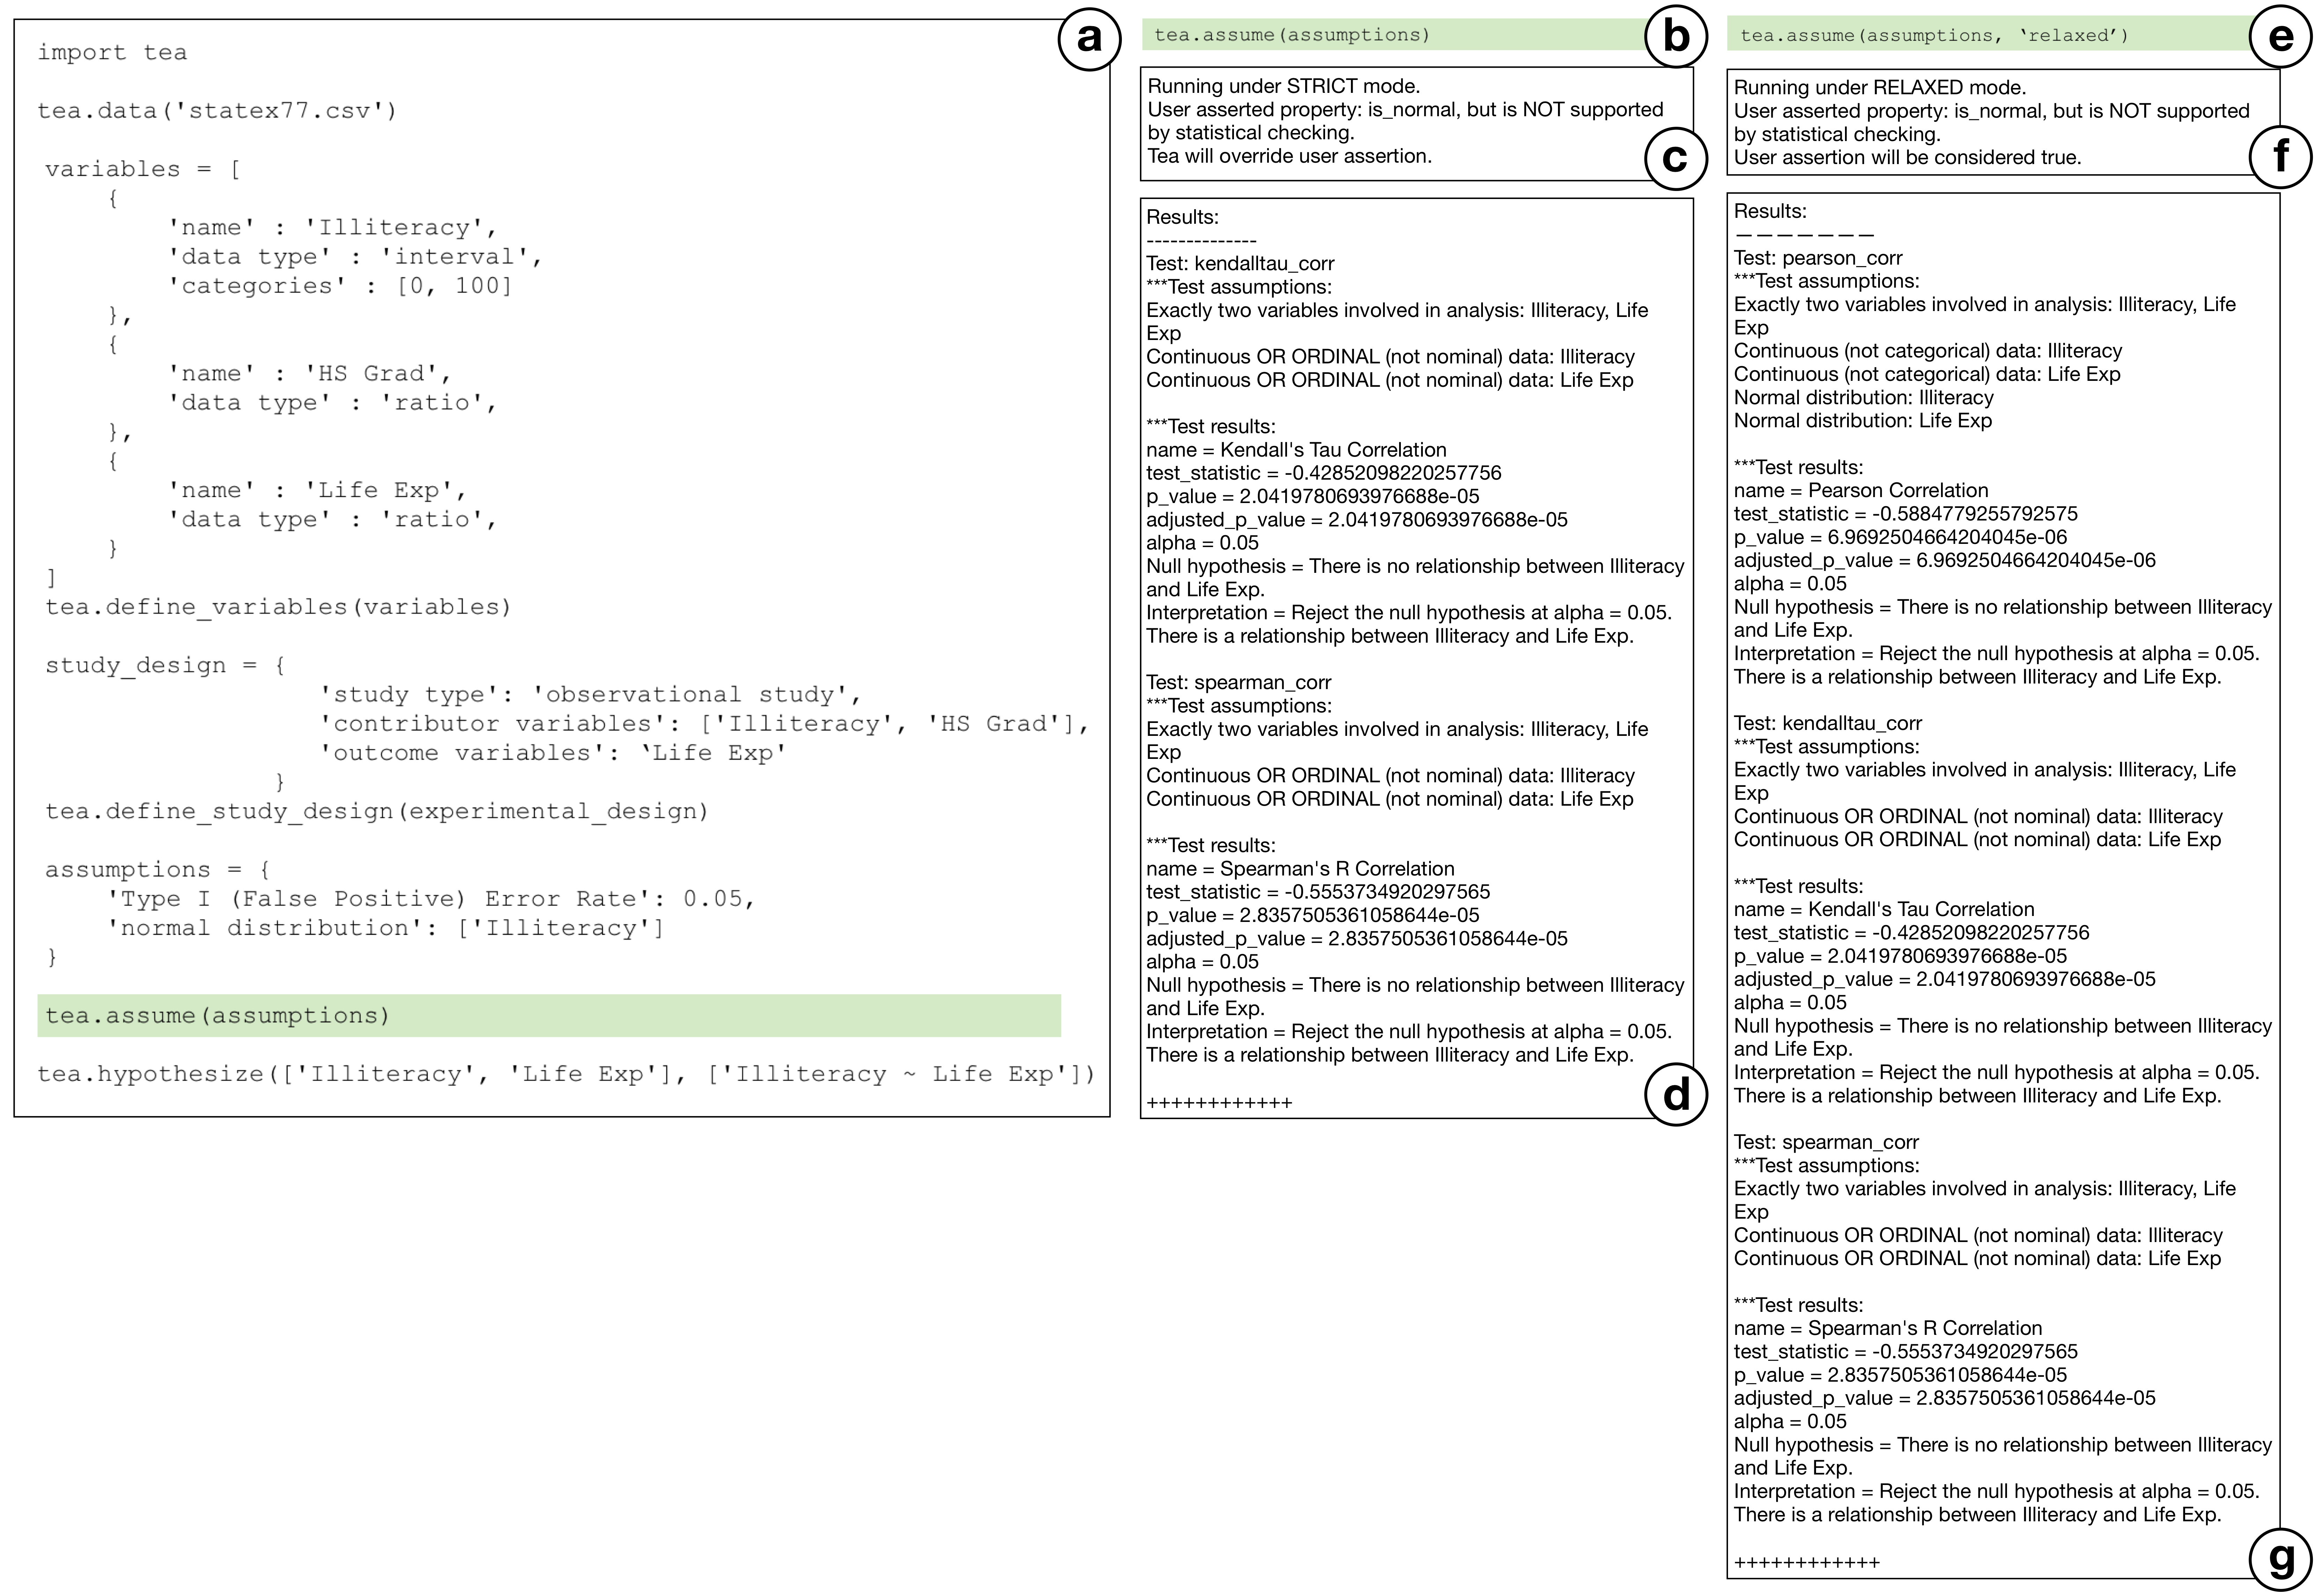
\includegraphics[width=\textwidth]{tea/figures/modes_wide.jpg}
    \vspace{-10pt}
    \caption{\textbf{Tea program and its mode-dependent executions.}}
      \begin{small}
      \begin{minipage}{\linewidth}
        a) Tea program that aims to determine if two contributor variables, `Illiteracy` and `HS Grad' that may predict a third outcome variable `Life Exp', are correlated. The user asserts that `Illiteracy' is normally distributed. 
        b) By default, Tea executes programs in the \textit{strict} mode. 
        c) Warning that Tea disagrees with the user and will override the user's assertion that `Illiteracy' is normally distributed in the \textit{strict} mode. 
        d) Results without the parametric test since Tea overrides user's assertion. 
        e) A single line change can modify Tea to execute a program in \textit{relaxed} mode. 
        f) Warning that Tea cannot verify normality for `Illiteracy' but will defer to user's assertion. 
        g) Results with the parametric test since Tea proceeds as if  `Illiteracy' was normally distributed.
      \end{minipage}
      \end{small}
    \label{fig:modes}
    \vspace*{-\baselineskip}
  \end{figure}
}
 
\newcommand{\figureSyntacticSugar}{
  \begin{figure}
      \centering
      \subcaptionbox{Specify the test.}
      {\fbox{\includegraphics[width=\linewidth, clip]{tea/figures/sugar_test.jpg}}}
      \label{fig:sugar_expanded}
      \subcaptionbox{Specify the properties.}
      {\fbox{\includegraphics[width=\linewidth, clip]{tea/figures/sugar_expanded.jpg}}}
      \label{fig:sugar_test}
      % \vspace{-10pt}
    \caption{\textbf{Tea can support pre-registration.} Tea programs provide an executable format for pre-registration. When pre-registering studies, users can explicitly state their assumptions about data properties or specify the exact statistical test they intend to run with data. Specifying the name of a test (a) is \textit{syntactic sugar} for the more verbose form (b). The above code snippets are semantically equivalent.}
    \label{fig:sugar}  
    \vspace*{-\baselineskip}
    % \vspace{-3pt}
    \end{figure}
}

\def\r{Pearson's r\xspace}
\def\ktau{Kendall's $\tau$\xspace}
\def\srho{Spearman's $\rho$\xspace}
\def\pb{Pointbiserial\xspace}
\def\student{Student's t-test\xspace}
\def\paired{Paired t-test\xspace}
\def\mannu{Mann-Whitney U\xspace}
\def\wilcox{Wilcoxon signed rank\xspace}
\def\welch{Welch's t-test\xspace}
\def\f{F-test\xspace}
\def\rm{Repeated measures one way ANOVA\xspace}
\def\kw{Kruskal Wallis\xspace}
\def\friedman{Friedman\xspace}
\def\facANOVA{Factorial ANOVA\xspace}
\def\twoANOVA{Two-way ANOVA\xspace}
\def\chiSq{Chi Square\xspace}
\def\fisher{Fisher's Exact\xspace}
\def\boot{Bootstrap\xspace}

\lstdefinestyle{teastyle}{
    backgroundcolor=\color{white},
    commentstyle=\color{codegreen},
    keywordstyle=\color{magenta},
    numberstyle=\tiny\color{codegray},
    stringstyle=\color{codepurple},
    basicstyle=\ttfamily\footnotesize,
    breakatwhitespace=false,
    breaklines=true,
    captionpos=b,
    keepspaces=true,
    numbers=left,
    numbersep=5pt,
    showspaces=false,
    showstringspaces=false,
    showtabs=false,
    tabsize=2,
    deletekeywords={input, print, id},
    % alsoletter={_},
    % literate={define_variables}{\textcolor{magenta}{define\_variables}}1,
    otherkeywords={tea.data, tea.define_variables, tea.define_study_design, tea.assume, tea.hypothesize}
    % here are the additional keywords
%     emph={data, define_variables, define_study_design, assume, hypothesize, <, >, =, !},
    % they are underlines
%     emphstyle={\textbf}
}

\newcommand{\figureTeaProgram}{
  % \lstset{deletekeywords={hypothesize}}
  \lstinputlisting[
        style=teastyle,
        % language=Python, 
        % keywordstyle=\color{black},  % choose your preferred color
        % morekeywords={},
        caption={\textbf{Sample Tea program.} 
        The specification outlines an observational study to analyze the relationship between geographic location (`So') and probability of imprisonment (`Prob') in a common USCrime data set~\protect\cite{venables2013modern,kabacoff2011action}. 
        See~\autoref{usageScenarioTea} for an explanation of the code. Tea programs specify 1) data, 2) variables, 3) study design, 4) assumptions, and 5) hypotheses.
        % \end{small}
        },
        label={lst:tea_program}
  ]{tea/figures/tea-example.py}

  % \renewcommand{\theFancyVerbLine}{
  % \sffamily\textcolor[rgb]{0.5,0.5,0.5}{\scriptsize\arabic{FancyVerbLine}}}

  % \begin{minted}[mathescape,
  %               linenos,
  %               numbersep=5pt,
  %               gobble=2,
  %               frame=lines,
  %               framesep=2mm]{csharp}
  %   string title = "This is a Unicode π in the sky"
  %   /*
  %   Defined as $\pi=\lim_{n\to\infty}\frac{P_n}{d}$ where $P$ is the perimeter
  %   of an $n$-sided regular polygon circumscribing a
  %   circle of diameter $d$.
  %   */
  %   const double pi = 3.1415926535
  % \end{minted}


% \begin{figure}
%     % \vspace{-5pt}
%     \centering
%     \includegraphics[width=0.5\columnwidth, clip]{tea/figures/tea_program.jpg}
%     % \vspace{-15pt} 
%     \caption{\textbf{Sample Tea program.}}
%       \begin{small}
%       \begin{minipage}{\linewidth}
%         The specification outlines an experiment to analyze the relationship between geographic location (`So') and probability of imprisonment (`Prob') in a common USCrime data set~\protect\cite{venables2013modern,kabacoff2011action}.
%         See~\autoref{usageScenarioTea} for an explanation of the code. Tea programs specify 1) data, 2) variables, 3) study design, 4) assumptions, and 5) hypotheses.
%       \end{minipage}
%       \end{small} 
%     \label{lst:tea_program}
%     \vspace{-\baselineskip}
% \end{figure}
}


\def\r{Pearson's r}
\def\ktau{Kendall's $\tau$}
\def\srho{Spearman's $\rho$}
\def\pb{Pointbiserial}
\def\student{Student's t-test}
\def\paired{Paired t-test}
\def\mannu{Mann-Whitney U}
\def\wilcox{Wilcoxon signed rank}
\def\welch{Welch's}
\def\f{F-test}
\def\rm{Repeated measures one way ANOVA}
\def\kw{Kruskal Wallis}
\def\friedman{Friedman}
\def\facANOVA{Factorial ANOVA}
\def\twoANOVA{Two-way ANOVA}
\def\chiSq{Chi Square}
\def\fisher{Fisher's Exact}

\newcommand{\tableTeaTests}{
    \begin{table*}[htbp]
      \begin{center} \singlespacing
      \caption{Statistical tests supported in Tea's Null Hypothesis Significance Testing module} \label{tab:tea_tests}
      \begin{tabular}{lll}
      \toprule
      \colH{Class of tests}           & \colH{Parametric} & \colH{Non-parametric} \\
        Correlation                   & \r                &  \ktau   \\
                                      & \pb               &  \srho  \\
        \midrule
        Bivariate mean comparison     & \student          & \welch \\
                                      &                   & \mannu \\
                                      &                   & (a.k.a. Wilcoxon rank sum) \\
                                      & \paired           & \wilcox \\
        \midrule
        Multivariate mean comparison  & \f                & \kw   \\
                                      & \rm               & \friedman \\
                                      & \twoANOVA         & \\
                                      & \facANOVA         & \\
        \midrule
        \midrule
        Proportions: \chiSq , \fisher and Others: Bootstrapping (with confidence intervals) \\
      \bottomrule
      \end{tabular}
      \end{center}
    \end{table*}
}

\newcommand{\furtherTestResults}{
\begin{table*}[htbp]
  \begin{center}
    \caption{Results from Factorial ANOVA for RM ANOVA example.}
    \begin{tabularx}{\linewidth}{XXXXXX}
       & \textbf{df} & \textbf{sum\_sq} & \textbf{mean\_sq} & \textbf{F} & \textbf{PR(>F)} \\
      C(conc) & 6.0 & 4068.771429 & 678.128571 & 9.261087 & 1.242777e-07 \\
      Residual & 77.0 & 5638.204167  & 73.223431   &    NaN     &      NaN \\
    \end{tabularx}
    \end{center}
    \label{tab:rm_anova_fanova}
\end{table*}

\begin{table*}[htpb]
  \begin{center}
    \caption{Results from F test for F test example.}
    \begin{tabularx}{\linewidth}{XXXXXX}
       & \textbf{df} & \textbf{sum\_sq} & \textbf{mean\_sq} & \textbf{F} & \textbf{PR(>F)} \\
        C(trt)   &  4.0 & 1351.369014 & 337.842253 & 32.432826 & 9.818516e-13 \\
        Residual & 45.0 &  468.750438  & 10.416676    &    NaN       &    NaN \\
    \end{tabularx}
  \end{center}
  \label{tab:f_test_f_test}
\end{table*}

\begin{table*}[htpb]
  \begin{center}
    \caption{Results from Factorial ANOVA test for F test example.}
    \begin{tabularx}{\linewidth}{XXXXXX}
       & \textbf{df} & \textbf{sum\_sq} & \textbf{mean\_sq} & \textbf{F} & \textbf{PR(>F)} \\
        C(trt)   &  4.0 & 1351.369014 & 337.842253 & 32.432826 & 9.818516e-13 \\
        Residual & 45.0 &  468.750438  & 10.416676    &    NaN       &    NaN \\
    \end{tabularx}
  \end{center}
  \label{tab:f_test_fanova}
\end{table*}

\begin{table*}[htpb]
  \begin{center}
    \caption{Results from Factorial ANOVA test for Paired T test example.}
    \begin{tabularx}{\linewidth}{XXXXXX}
       & \textbf{df} & \textbf{sum\_sq} & \textbf{mean\_sq} & \textbf{F} & \textbf{PR(>F)} \\
        C(Group) &  1.0 &  294.0  &  294.0 & 2.826923 & 0.106839 \\
        Residual & 22.0 & 2288.0  &  104.0    &   NaN   &    NaN \\
    \end{tabularx}
  \end{center}
  \label{tab:paired_t_fanova}
\end{table*}


\begin{table*}[htpb]
  \begin{center}
    \caption{Results from F test and Factorial ANOVA for Student's T test example.}
    \begin{tabularx}{\linewidth}{XXXXXX}
       & \textbf{df} & \textbf{sum\_sq} & \textbf{mean\_sq} & \textbf{F} & \textbf{PR(>F)} \\
        C(So)   &   1.0 &  0.006702 &  0.006702 & 17.657903 & 0.000124 \\
        Residual & 45.0 & 0.017079 & 0.000380    &    NaN     &  NaN \\
    \end{tabularx}
  \end{center}
  \label{tab:students_t_f_test_and_fanova}
\end{table*}
}

\begin{comment}
% make a custom style that looks good and can highlight some additional keywords
\lstdefinestyle{tea}{
  basicstyle=\ttfamily,
  deletekeywords={input, print, id},
  language=Python,
  % here are the additional keywords
  emph={data, define_variables, define_study_design, assume, hypothesize, <, >, =, !},
  % they are underlines
  emphstyle={\bf},
}
\lstset{
  % use this style by default
  style=tea,
  % look better
  columns=flexible,
  showstringspaces=false,
  % spacing, size, numbers, etc.
  numbers=left,
  xleftmargin=2em,
  numberstyle=\tiny,
  escapechar=|,
}
\end{comment}

\newcommand{\teaHypotheses}{
  \begin{figure}[t]
    \vspace{-5pt}
    \centering
    \includegraphics[width=1.\columnwidth, clip]{tea/figures/tea_hypotheses.png}
    % \vspace{-15pt}
    \caption{\textbf{Hypotheses that users can express in Tea.} }
    \label{fig:teaHypotheses}
    \vspace{-\baselineskip}
    \vspace{-3pt}
  \end{figure}
}


\newcommand{\otherSystems}{
    \begin{table*}[t]
        \centering \small
        \caption{\textbf{Comparison of Tea to other tools.}}
          \begin{small}
          \begin{minipage}{\linewidth}
            Despite the published best practices for statistical analyses, most
            tools do not help users select appropriate tests. Tea not only
            addresses the best practices but also supports reproducing analyses.
            Below, $\sim$ indicates a practice is sometimes supported.
          \end{minipage}
          \end{small}
        \label{tab:otherSystems}
        \begin{tabularx}{\linewidth}{r|c|c|c|c|c|c}
          \toprule
            \colHR{Best practices} & \colH{SAS} & \colH{SPSS} & \colH{JMP} & \colH{R} & \colH{\makecell{Statsplorer\\\cite{wacharamanotham2015statsplorer}}} & \colH{Tea} \\
            \midrule \\ 
            % & & & & & \colH{\cite{wacharamanotham2015statsplorer}} & \\
            % \midrule \\ 
            Explicit statement of user assumptions & \no & \no & \no & \no & \no & \yes \\
            Automatic verification of test preconditions & \no & \no & $\sim$ & $\sim$ & \yes & \yes \\
            Automatic accounting of multiple comparisons & \no & \no & \no & \no & \yes & \yes \\
            Surface alternative analyses & \no & \no & \no & \no & \no & \yes \\
            Contextualize results & \yes & $\sim$ & \yes & $\sim$ & \yes & \yes \\
            Easy to reproduce analysis & \yes & \yes & \no & \yes & \no & \yes \\
        \end{tabularx}
    \end{table*}
}


\newcommand{\figureOutputTTest}{
  \begin{figure}[t]
    \vspace{-15pt}
    % \centering
    \fbox{\includegraphics[width=.8\columnwidth, clip]{tea/figures/tea_output_t_test.jpg}}
    \vspace{2pt}
    \caption{\textbf{Part of Tea's output.} The output is a result of running the sample program in \autoref{lst:tea_program}. Tea outputs the data properties that led Tea to select the statistical test as well as results from executing the test, effect size calculations, the null hypothesis tested, and the interpretation of the results, which can be included in publications with minor editing.}
    \label{fig:output_t_test}
    \vspace*{-\baselineskip}
    \vspace{-15pt}
  \end{figure}
}

\newcommand{\figureModes}{
  \begin{figure}[H]
    % \vspace{-5pt}
    \centering
    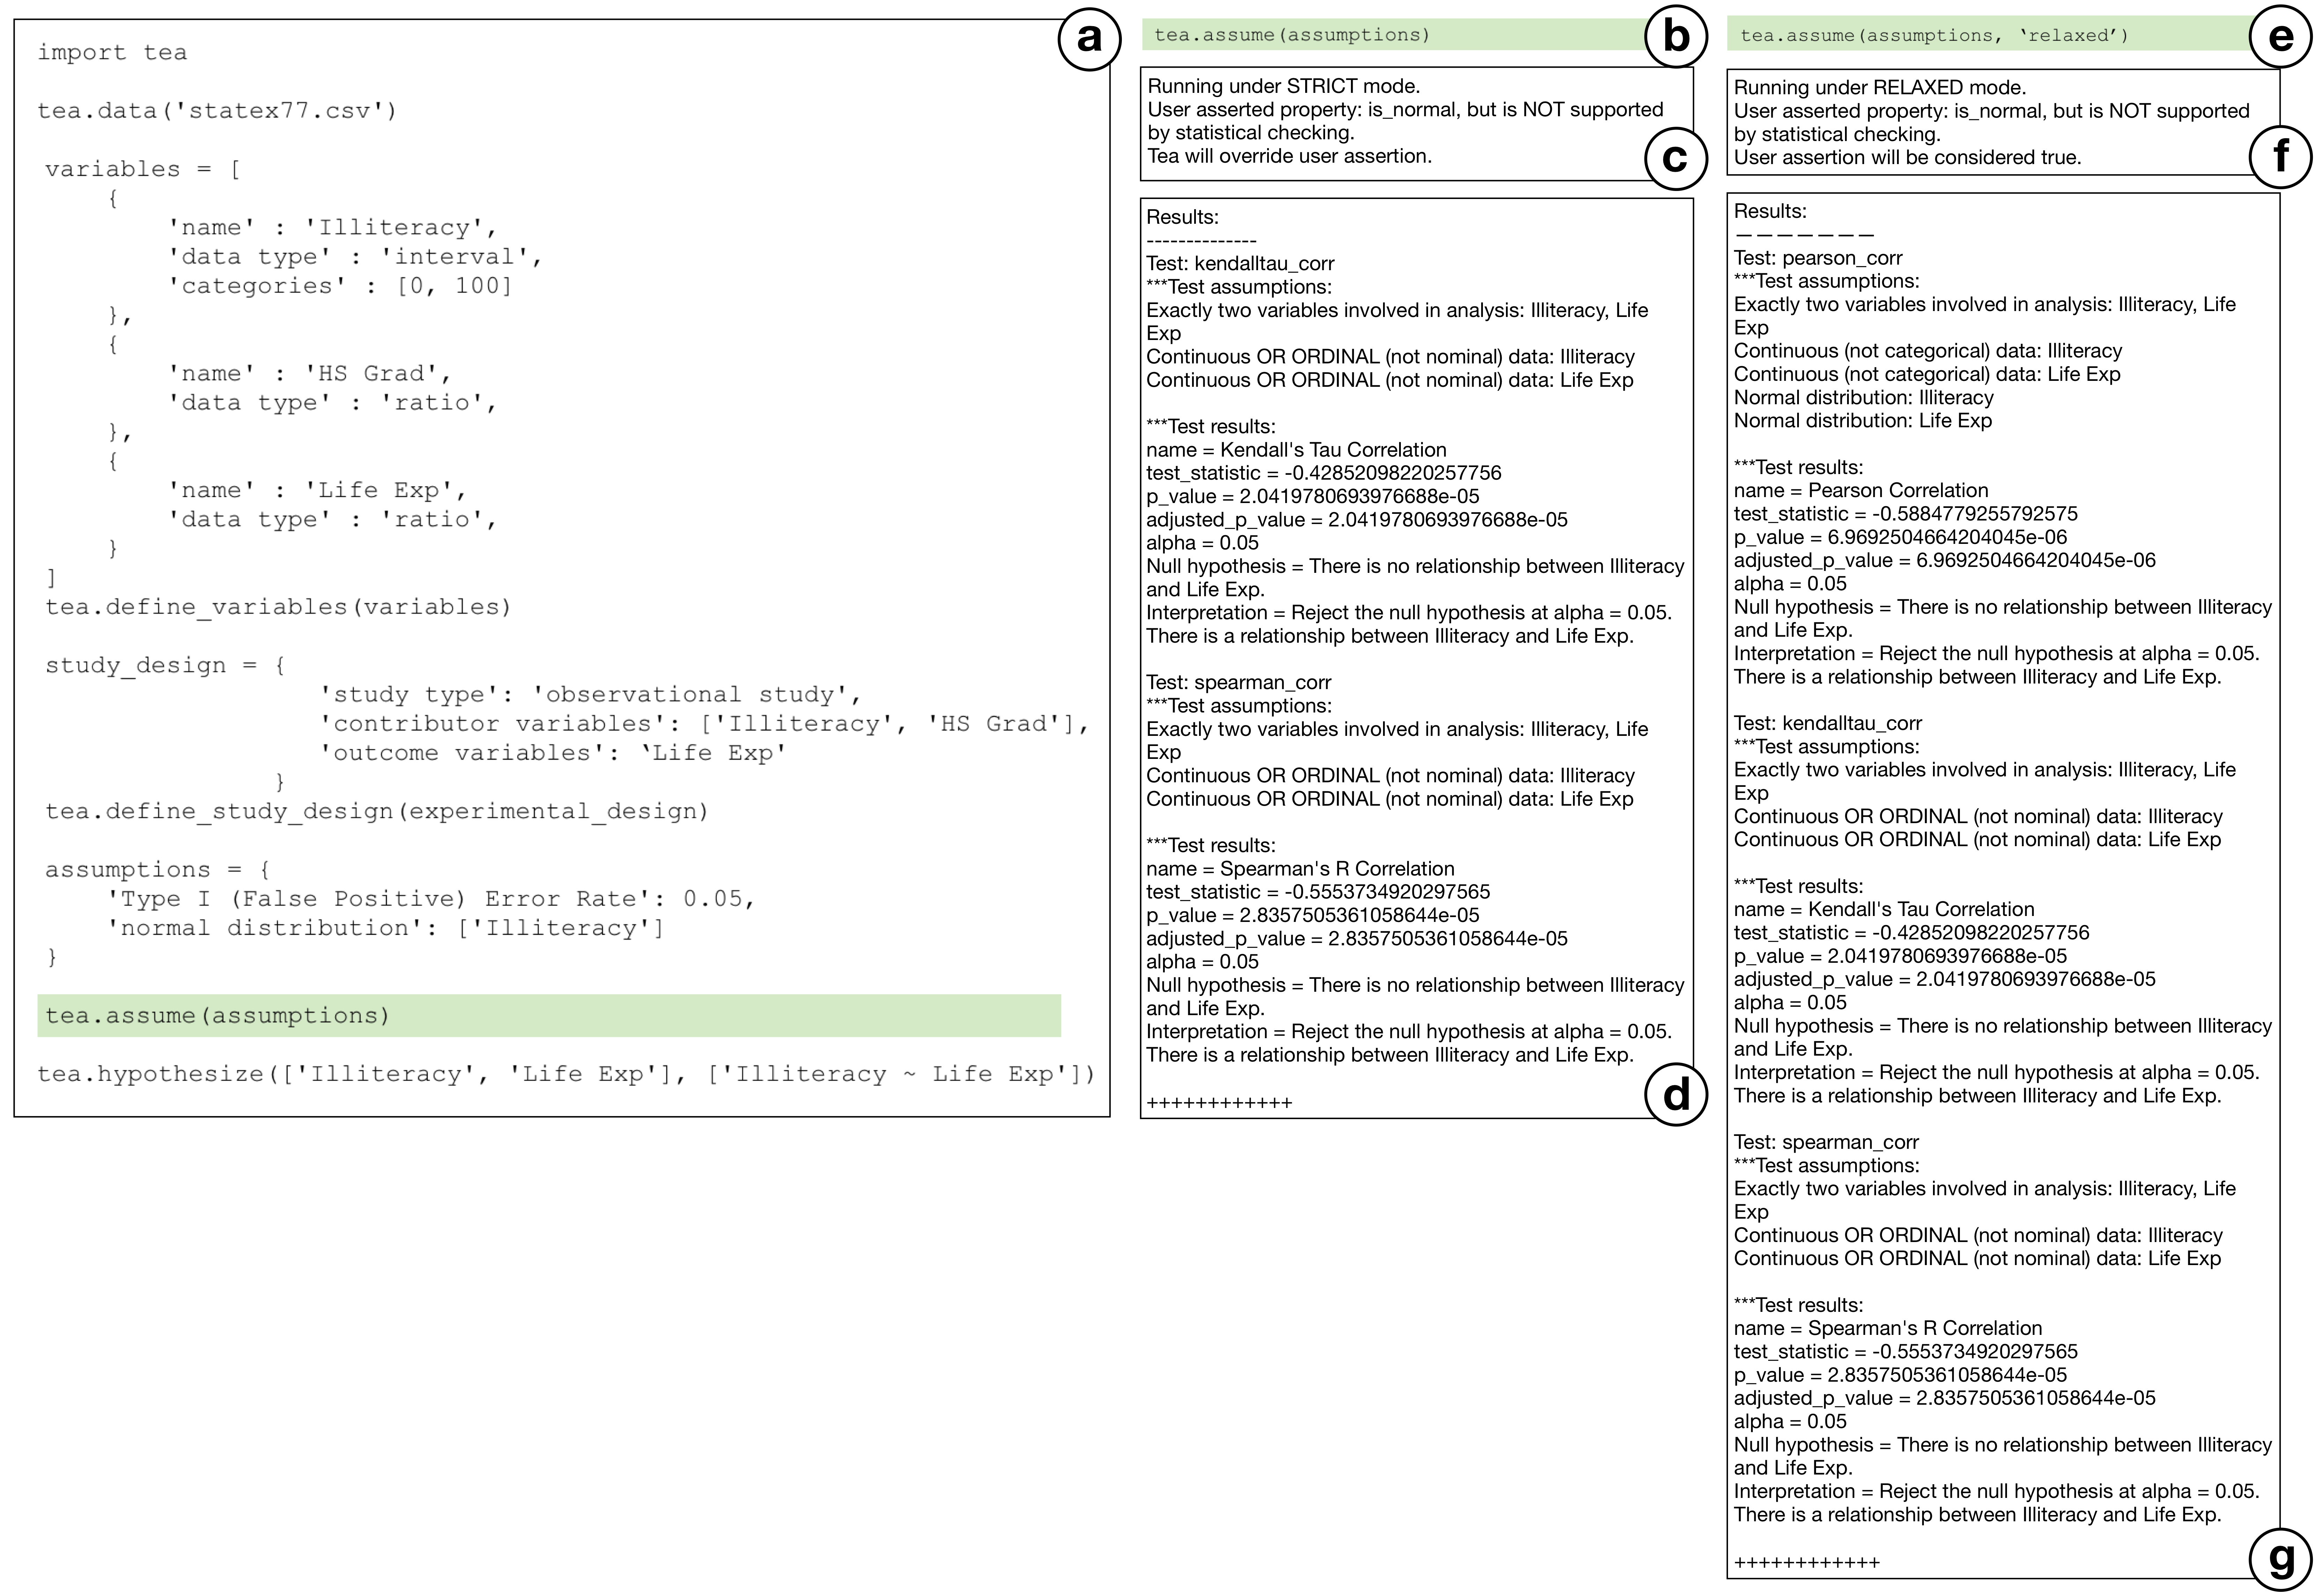
\includegraphics[width=\textwidth]{tea/figures/modes_wide.jpg}
    \vspace{-10pt}
    \caption{\textbf{Tea program and its mode-dependent executions.}}
      \begin{small}
      \begin{minipage}{\linewidth}
        a) Tea program that aims to determine if two contributor variables, `Illiteracy` and `HS Grad' that may predict a third outcome variable `Life Exp', are correlated. The user asserts that `Illiteracy' is normally distributed. 
        b) By default, Tea executes programs in the \textit{strict} mode. 
        c) Warning that Tea disagrees with the user and will override the user's assertion that `Illiteracy' is normally distributed in the \textit{strict} mode. 
        d) Results without the parametric test since Tea overrides user's assertion. 
        e) A single line change can modify Tea to execute a program in \textit{relaxed} mode. 
        f) Warning that Tea cannot verify normality for `Illiteracy' but will defer to user's assertion. 
        g) Results with the parametric test since Tea proceeds as if  `Illiteracy' was normally distributed.
      \end{minipage}
      \end{small}
    \label{fig:modes}
    \vspace*{-\baselineskip}
  \end{figure}
}
 
\newcommand{\figureSyntacticSugar}{
  \begin{figure}
      \centering
      \subcaptionbox{Specify the test.}
      {\fbox{\includegraphics[width=\linewidth, clip]{tea/figures/sugar_test.jpg}}}
      \label{fig:sugar_expanded}
      \subcaptionbox{Specify the properties.}
      {\fbox{\includegraphics[width=\linewidth, clip]{tea/figures/sugar_expanded.jpg}}}
      \label{fig:sugar_test}
      % \vspace{-10pt}
    \caption{\textbf{Tea can support pre-registration.} Tea programs provide an executable format for pre-registration. When pre-registering studies, users can explicitly state their assumptions about data properties or specify the exact statistical test they intend to run with data. Specifying the name of a test (a) is \textit{syntactic sugar} for the more verbose form (b). The above code snippets are semantically equivalent.}
    \label{fig:sugar}  
    \vspace*{-\baselineskip}
    % \vspace{-3pt}
    \end{figure}
}

\newcommand{\formula}{Formula}
\newcommand{\assignRoles}{Specify variable roles}

\def\arraystretch{0.35}
\newcommand{\tableSoftwareAnalysis}{
    \begin{table*}
        \footnotesize
        \caption{\textbf{Overview of the software tools included in our analysis.}\label{tableAnalysisOfTools}}
        \begin{small}
        \vspace*{-10pt}
        \begin{minipage}{\linewidth}
        Half of the tools
        are specialized for specific modeling use cases. Most tools
        use mathematical notation (T18--T20 (\yes*) even use
        mathematical notation in their GUIs).
        Most tools also provide a wide range
        of computational control although sometimes they require additional
        packages [T5, T13]. Tool specialization, organization,
        notation, and computational control focus analysts on model
        implementation details, sometimes at the expense of focusing on their conceptual
        hypotheses.
        \end{minipage}
        \end{small}
        
        \setlength{\tabcolsep}{4pt}
        \begin{tabular}{l>{\raggedright}p{0.3\linewidth}p{0.15\linewidth}p{0.15\linewidth}p{0.15\linewidth}p{0.2\linewidth}}
        \toprule
        ID & Tool name                                          & Specialized Scope    & Mathematical Notation        & Computational Control            & References                               \\                     
        \multicolumn{2}{l}{\textbf{R Packages}} \\
        \midrule\\
        T1 & MASS                                               & \no                  & \yes                         & \yes                             & ~\cite{mass}                                 \\                     
        T2 & brms                                               & \yes                 & \yes                         & \yes                             & ~\cite{burkner2017brms,brmsRef}                                 \\                     
        T3 & edgeR                                              & \yes                  & \yes                        & \yes                            & ~\cite{edgeROverview,edgeRUsersGuide}                                 \\                     
        T4 & glmmTMB                                            & \yes                 & \yes                         & \yes                             & ~\cite{glmmtmbPaper,glmmtmbRef}                                 \\                     
        T5 & glmnet                                             & \yes                 & \no                          & \yes (additional)                & ~\cite{glmnetRef,glmnetVignette}                                 \\                     
        T6 & lme4                                               & \yes                 & \yes                         & \yes                             & ~\cite{bates2014fittingLme4,bates2014lme4Ref}                                 \\                     
        T7 & MCMCglmm                                           & \yes                 & \yes                         & \yes                             & ~\cite{MCMCglmmPaper,MCMCglmmRef}                                 \\                     
        T8 & nlme                                               & \yes                 & \yes                         & \yes                             & ~\cite{nlmeRef}                                 \\                     
        T9 & RandomForest                                       & \yes                 & \yes                         & \yes (minimal)                   & ~\cite{randomForestR}                                 \\                     
        T10 & stats (core library)                              & \no                  & \yes                         & \yes                             & ~\cite{statsCoreRRef}                                 \\                     
        \multicolumn{2}{l}{\textbf{Python Packages}} \\                 
        \midrule\\                  
        T11 & Keras                                             & \yes                 & \no                          & \yes (minimal)                   & ~\cite{keras}                                 \\                     
        T12 & Scikit-learn                                      & \yes                 & \no                          & \yes                             & ~\cite{scikitRef,scikitPaper,scikitAPIPaper}                                 \\                                                                            
        T13 & Scipy (scipy.stats)                               & \no                  & \no                          & \yes (additional)                & ~\cite{scipy,scipyStats,scipyOptimize}                                 \\                     
        T14 & Statsmodels                                       & \no                  & \yes                         & \no                              & ~\cite{statsmodelsPaper,statsmodelsRef}                                 \\                                                                                  
        \multicolumn{2}{l}{\textbf{Suites, with DSLs for programming}} \\                   
        \midrule\\                  
        T15 & Matlab (Statistics and ML Toolbox)                & \no                  & \no                          & \yes                             & ~\cite{matlab,matlabStats}                                 \\                     
        T16 & SPSS                                              & \no                  & \yes                         & \yes                             & ~\cite{spss}                                 \\                                    
        T17 & Stata                                             & \no                  & \yes                         & \no                              & ~\cite{stata,stataRef,stataLang}                                 \\                     
        \multicolumn{2}{l}{\textbf{Suites, without programming}} \\                 
        \midrule\\                  
        T18 & GraphPrism                                        & \no                  & \yes *                       & \yes                             & ~\cite{graphPadUserGuide}                                 \\                                    
        T19 & JASP                                              & \no                  & \yes *                       & \no                              & ~\cite{jasp}                                 \\                                    
        T20 & JMP                                               & \no                  & \yes *                       & \no                              & ~\cite{jmp,jones2011jmp}                                 \\                                                                                  
        \bottomrule 
        \end{tabular}
        \vspace{-4mm}
        \end{table*}
        
}

\newcommand{\figureOverivew}{
    \begin{figure}[h]
        \centering
        \includegraphics[width=.8\textwidth]{hypothesisFormalization/figures/overview_sept_17.png}
        \caption{\textbf{Definition and overview of the hypothesis formalization
        steps and process.}\label{figure:hypoFormOverview}}
        \begin{small}
        \begin{minipage}{\linewidth}
        Hypothesis formalization is a dual-search process of
        translating a \textbf{conceptual hypothesis} into a statistical
        \textbf{model implementation}.
        %
        Blue indicates steps and transitions that we identified.
        Black indicates steps and transitions discussed in prior work.
        ``Mathematical Equation'' (dashed box) was rarely an explicit step in
        our lab study but evident in our content analysis.
        Our findings (blue arrows) corroborate and subsume several of the transitions identified
        in prior work with greater granularity. When they do not, prior work's transitions are included in black.
        For example, analysts may operationalize a conceptual hypothesis as a causal model by first decomposing the conceptual hypothesis into sub-hypotheses and then identifying proxy variables to incorporate in a causal model (blue arrows above).
        Our definition of hypothesis formalization is a consequence of our synthesis of prior work, content analysis, lab study, and analysis of tools.
        % 
        Hypothesis formalization is a non-linear process.
        Analysts iterate over conceptual steps to refine their hypothesis in a
        \textit{hypothesis refinement loop}.
        Analysts also iterate over computational and implementation steps in a
        \textit{model implementation loop}.
        Data collection and data properties may also prompt conceptual revisions
        and influence statistical model implementation.
        %
        As analysts move toward model implementation, they increasingly rely on
        software tools, gain specificity, and create intermediate artifacts
        along the way (e.g., causal models, observations about data, etc.).
        % that help them satisfy conceptual, data, statistical, and computational constraints.
        \end{minipage}
        \end{small}
      \end{figure}
}

\newcommand{\figurePriorWorkCombined}{
    \begin{figure}[ht]
        \centering
        \includegraphics[width=0.8\textwidth]{hypothesisFormalization/figures/prior_work_combined_july_16_2021.png}
        \caption{\textbf{Relationship between hypothesis formalization and prior work.}\label{figure:priorWork}}
        \begin{small}
        \begin{minipage}{\linewidth}
         \textit{Left:}
        Schunn and
        Klahr's four-space model of scientific
        discovery (stylized adaptation from  Figure 1 in~\cite{schunn1995FourSpace}),
        which includes unidirectional information flow
        from the hypothesis space to the paradigm space (which includes
        model implementation). Hypothesis formalization (A) is focused on a
        tighter integration and the information flow between hypothesis and paradigm spaces.
        Specifically, the information flow is bidirectional in hypothesis formalization.
        Our content analysis (B) and lab study (C) triangulate the four-space
        model to understand hypothesis formalization
        from complementary perspectives.
        \textit{Right:} Hypothesis formalization steps also identified in
        prior work on theories of
        sensemaking, statistical thinking, and data analysis workflows (citations included to the right of the arrows).
        Hypothesis formalization is finer grained and involves more iterations.
        While prior work broadly refers to mathematical equations,
        partial model specifications, and computationally tuned model
        implementations as statistical specifications, hypothesis formalization
        differentiates them. As a whole, this chapter provides empirical evidence for
        theorized loops between conceptual hypothesis and statistical
        specification (see Figure~\ref{figure:hypoFormOverview}).
        \end{minipage}
        \end{small}
        \vspace*{-15pt}
      \end{figure}
    % \begin{figure}
    %     \centering
    %     \begin{subfigure}{.5\textwidth}
    %         \centering
    %         \includegraphics[width=.5\textwidth]{hypothesisFormalization/figures/methods_overview.png}
    %         \caption{A subfigure}
    %         \label{fig:sub1}
    %     \end{subfigure}%
    %     \begin{subfigure}{.5\textwidth}
    %         \centering
    %         \includegraphics[width=.5\textwidth]{hypothesisFormalization/figures/prior_work_sept_11.png}
    %         \caption{A subfigure}
    %         \label{fig:sub2}
    %     \end{subfigure}
    %     \caption{A figure with two subfigures}
    %     \label{fig:test}
    % \end{figure}
}

\newcommand{\figureLabStudyStatSpec}{
    \begin{figure}
        \centering
        \begin{minipage}{0.45\textwidth}
            \centering
            \includegraphics[width=0.9\textwidth]{hypothesisFormalization/figures/A11_SS_1.png} % first figure itself
        \end{minipage}\hfill
        \begin{minipage}{0.45\textwidth}
            \centering
            \includegraphics[width=0.9\textwidth]{hypothesisFormalization/figures/A11_SS_2.png} % second figure itself
        \end{minipage}
        \caption{\textbf{Sample statistical specification (D8).}\label{figure:labStudyStatSpec}}
            \begin{small}
            \begin{minipage}{\linewidth}
            The lab study tasked analysts
            to specify their statistical models without
            considering implementation. 
            We expected analysts would represent
            their statistical models using statistical test names or mathematical equations. 
            %their statistical models mathematically. 
            Instead, most analysts specified statistical procedures for performing statistical models 
            using todo lists and summaries of steps,
            which sometimes included mentions of software tools, showing that
            implementation was an important consideration and
            that tool familiarity may limit which statistical models
            analysts consider and implement.
            Data worker D8 specified their model through a combination of statistical test names (e.g., Chi-squared test) and a list (split across two pages) of detailed steps
            involved in creating new variables, cleaning and wrangling data,
            visualizing data, and testing their hypothesis. 
            \end{minipage}
            \end{small}
    \end{figure}
}

\newcommand{\figureExampleReorderableMatrix}{
    \begin{figure}
        \centering
        \includegraphics[width=0.9\textwidth]{hypothesisFormalization/figures/ps9_reorderableMatrixLabeled.png}
        \caption{\textbf{Formative content analysis: example reorderable matrix for~\cite{PS9}.}\label{figure:exampleReorderableMatrix}}
        \begin{small}
            \begin{minipage}{\linewidth}
            %
            We visualized each paper in our sample as a ``reorderable
            matrix''~\cite{bertin2011graphics} to aid in detecting patterns in
            papers' structure and content that could indicate how researchers
            formalized their hypotheses. The rows represent the codes in our
            codebook, colored according to the five broad categories of codes:
            research goals (rows 1-5, green), sample information (rows 6-9,
            orange), statistical analysis details (rows 10-12, red), reporting
            of results (rows 13-18, blue), and computational details (rows
            19-20, bright yellow). The columns are the paragraphs, which are indexed by
            their first sentences, ordered left to right. In a paragraph's
            column, there is an ``X'' for each code the paragraph received.
            Paragraphs have multiple codes if they contain multiple types of
            information. 
            %
            Among the ten visual patterns we noticed across our sample and
            subsequently looked for in each paper, two stand out in this paper.
            (A) As the paper progresses (visually moving left to right), the
            paper's focus shifts from research goals to sample information to
            statistical analysis to results, as indicated by the arrow labeled
            A. Largely expected, this pattern helps to validate our coding
            method. Also, there is only one paragraph that discusses statistical
            software. (B) Researchers discuss research goals and questions
            throughout the paper. Interestingly, in the middle of the paper,
            when the researchers discuss their goals in greater detail, the
            researchers discuss them in increasing specificity, as indicated by
            the arrow labeled B. We were able to detect this pattern across
            papers by iterating on how to order the research goal codes (rows
            1-5, green). The final order lists codes in increasing specificity
            from top (row 1) to bottom (row 5). Pattern B suggests that
            researchers refine their hypotheses during hypothesis formalization,
            which may involve specifying proxies and statistical methods.
            %
            The appendix discusses additional patterns in this paper
            and across our entire sample. 
            \end{minipage}
        \end{small}
    \end{figure}
}
% tisane/figures/tables to include:
% [usage scenario] 1. Overview of Tisane code, showcase all language constructs through multiple examples --> usage scenario (Pigs), appendix (Barr)
% [usage scenario] 2. Overview of disambiguation --> Pigs, Barr (random effects or family/link tabs)
% [draft] 3. Table describing clustering examples
% [] 4. Table/figure comparing existing tools with Tisane in terms of who is in charge of validity (row of checkboxes that say system does or system-human hybrid collab)
% 5. Overview of system workflow/interaction (language, representation, diambiguation, code generation, interactive compilation process is the entire thing)

%\def\myequation{$Y = \beta_{0} + \beta_{1} X_{1} + \cdots + \beta_{n} X_{n}$}

\newcommand{\figureSystemOverview}{
%    \pgfplotstableread[col sep = comma]{tisane/figures/resid_plot.csv}\loadedtable

    \begin{figure*}%[h]
        \centering
\includegraphics{tisane/figures/figure1}
%        \begin{tikzpicture}[>=Stealth,
%                            every node/.style={node distance=0.5cm}]
%            \begin{scope}[local bounding box=bb,
%                          every node/.style={inner sep=5pt, node distance=0.5cm},
%                          stage/.style={fill=gray!10,rounded corners=4pt},
%                          caption/.style={node distance=.2cm,rounded corners=4pt}]
%                % \node[stage] (input) at (0, 0) {\includegraphics[width=.13\textwidth]{tisane/figures/tisane_code_icon}};
%                \node[stage] (input) at (0, 0) {\begin{tikzpicture}[every node/.style={inner sep=0pt},
%                                                                    button/.style={circle,minimum size=3pt}]
%                    \node[rectangle split, rectangle split parts=2, rounded corners=1pt, rectangle split part fill={tisanecodetop,white},rectangle split empty part height=7pt,inner sep=0pt,draw=gray!80,rectangle split draw splits=false] (n) {\nodepart{two} \begin{tikzpicture}
%                        \node[inner sep=5pt,rectangle, minimum height=1.5cm]       {\footnotesize \texttt{import tisane as ts}};
%                    \end{tikzpicture}};
%                    \coordinate (start) at ($(n.text west)+(4pt,0)$);
%                    \node[button,fill=closecolor]   (close) at (start) {};
%                    \node[button,fill=minimizecolor,right=0.5pt of close] (minimize) {};
%                    \node[button,fill=maximizecolor,right=0.5pt of minimize] (maximize) {};
%                \end{tikzpicture}};
%                % \node[caption,below=of input]   {\textit{Input Study Design specification}};
%                \node[right=of input,stage] (graphir) {\begin{tikzpicture}[every node/.style={circle, draw=black,fill=white}]
%                    \node (a) at (0,0) {};
%                    \node (b) at (-0.5, -1) {};
%                    \node (c) at (0.5, -1) {};
%                    \graph{
%                        (a) ->[densely dotted,bend right] (b);
%                        (c) ->[bend right] (a);
%                        (a) ->[bend right] (c);
%                        (c) ->[densely dashed,bend left] (b);
%                    };
%                \end{tikzpicture}};
%                % \node[caption,below=of graphir] (graphircaption) {\textit{Graph IR}};
%                \node[right=of graphir,stage] (disambig) {\includegraphics[width=.2\textwidth]{tisane/figures/tisane_screenshots/main_no_tooltip}};
%                % \node[below=.2cm of disambig,caption]    (disambigcaption) {\textit{Disambiguation}};
%                \node[right=of disambig,stage,text width=.2\textwidth,align=center] (code) {{\footnotesize \myequation}\\%
%                    \begin{tikzpicture}[every node/.style={rounded corners=0pt},rounded corners=0pt]
%                        \begin{axis}[rounded corners=0pt,
%                                     scatter/use mapped color={
%                                        fill=blue!80,
%                                        draw=blue!80
%                                     },
%                                     axis background/.style={fill=white},
%                                     xmin=-6.9,
%                                     xmax=6.9]
%                             \draw[gray,very thin] (axis cs:-5,-0.5) -- (axis cs:-5,0.5);
%                             \draw[gray,very thin] (axis cs:0,-0.5) -- (axis cs:0,0.5);
%                             \draw[gray,very thin] (axis cs:5,-0.5) -- (axis cs:5,0.5);
%                            \addplot[black,domain=-7:7] {0};
%                            \addplot[scatter,only marks,mark size=1.1pt] table[x=x,y=y,col sep=comma] {\loadedtable};
%                        \end{axis}
%                        \pgfresetboundingbox
%                        \path
%                                ($(current axis.south west)-(0.2cm,0.35cm)$) rectangle ($(current axis.north east)+(0,0.2cm)$);
%                    \end{tikzpicture}
%                };
%                \node   (codecaption) at ($(code.south)-(0,0.3cm)$)     {\textit{Output Code}};
%                \coordinate (ref) at ($(codecaption) + (0.5cm,0)$) {};
%                \node[caption]  (graphircaption1) at ($(codecaption)!(graphir)!(ref)$) {\textit{Graph IR}};
%                \node[caption]  (disambigcaption1) at ($(codecaption)!(disambig)!(ref)$) {\textit{Disambiguation}};
%                \node[caption]  (inputcaption)     at ($(codecaption)!(input)!(ref)$) {\textit{Input Study Design Specification}};
%                \graph{
%                    (input) ->[thick] (graphir) ->[thick] (disambig) ->[thick] (code);
%                };
%                \node at ($(current bounding box.south) + (0,-.4)$) {Interactive Compilation};
%                \node[color=white,inner sep=0pt] at ($(current bounding box.north) + (0,5pt)$) {};
%                \node[color=white,inner sep=0pt] (spacer) at ($(code.east)+(5pt,0)$) {};
%            \end{scope}
%
%            \begin{pgfonlayer}{background}
%                \node[rounded corners=4pt, draw=gray!50, fit=(bb)] {};
%                % \node[fill=gray!10, draw=none, fit=(bb)] {};
%            \end{pgfonlayer}
%            % \draw[fill=gray!30, draw=none] (current bounding box.north east) rectangle (current bounding box.south west);
%        \end{tikzpicture}
        \caption{\textbf{Overview of the Tisane system.} Analysts specify a set of variable relationships (\textit{Input Study Design Specification}). Tisane represents these in an internal graph (\textit{Graph IR}). To infer a statistical model, Tisane engages analysts in an interactive compilation process that elicits additional input from analysts in a disambiguation process (\textit{Disambiguation}) and outputs a script for fitting a valid GLM and visualizing its residuals (\textit{Output Code}).}
        \label{fig:figureSystemOverview}
        \Description{Four boxes (which we will refer to as A, B, C, and D) are shown in a row. Box A is labeled “Input Study Design Specification” and shows a text editor window where the text “import tisane as ts” is written (this is the canonical way of importing Tisane in Python, like “import pandas as pd”). Box A has an arrow pointing to Box B, which is labeled “Graph IR,” where “IR” stands for “intermediate representation.” Box B contains a directed graph with three nodes, arranged like the vertices of an isosceles triangle. The top node has a dotted arrow pointing toward the bottom left node and a solid arrow pointing at the bottom right node. The bottom right node has a dashed edge pointing toward the bottom left node and a solid edge pointing to the top node. The bottom left node has no outgoing edges. This is meant to be a icon for the Graph IR. Box B has an arrow pointing to Box C, which is labeled as “Disambiguation.” Box C contains a screenshot of the Tisane GUI. The top of the GUI has the word “Tisane” and a progress bar, which is a quarter blue and three quarters gray. A left side panel gives an overview of the current model, and shows variables expressed by the query (the dependent variable, pounds_lost, and the independent variables, treatment and motivation), the variables added (the query independent variables are listed underneath, while noting that there are no interactions to add), clustering variables (group, a random intercept), and that for data distributions, no family or link functions have been selected. Box C has an arrow pointing to Box D, which is labeled “Output Code”. The box contains an equation, Y = beta_0 + beta_1 X_1 + … + beta_n X_n, and below the equation is a plot of residuals vs. fitted values. This is meant to represent the output script that Tisane creates.}
    \end{figure*}
}

\newcommand{\figureGraphIRExample}{
    \begin{figure}[h]
\centering
\includegraphics{tisane/figures/figure4.pdf}
%        \begin{tikzpicture}[>=Stealth,
%                            causes/.style={thick,draw=black, "causes", text=black},
%                            associates/.style={thick,draw=black, "assoc."},
%                            min/.style={minimum size=1.5cm},
%                            unit/.style={min,draw=black},
%                            measure/.style={min,circle,draw=black},
%                            has/.style={densely dotted,thick},
%                            nests/.style={dashed,thick},
%                            depvar/.style={fill=gray!30},
%                            every edge quotes/.style={fill=none,fill opacity=.9,text opacity=1,rounded corners=3pt,inner sep=2pt},
%                            tightly/.style={inner sep=1pt},
%                            loosely/.style={inner sep=.7em}]
%            \node[unit]		(group) at (0,0)			{\texttt{group}};
%            \node[unit,right=3.5cm of group]	(member)		{\texttt{member}};
%            \node[measure,below=1.75cm of member]		(motivation)	{\texttt{motivation}};
%            \coordinate (ref1) at ($(motivation.center) + (1cm, 0)$) {};
%            \node[measure] at ($(ref1)!(group.center)!(motivation.center)$)		(condition)		{\texttt{condition}};
%
%
%            \coordinate (midcoord1) at ($(group.center)!0.5!(member.center)$) {};
%            \coordinate (midcoord2) at ($(member.center)!0.5!(motivation.center)$) {};
%            \coordinate (ref) at ($(midcoord2) + (1cm, 0)$) {};
%            \node[measure,depvar] at ($(midcoord2)!(midcoord1)!(ref)$)		(poundslost)	{\texttt{pounds\_lost}};
%            % \node[measure,above right=of motivation]		(age)			{\texttt{age}};
%
%            \graph
%        %			[edge quotes={fill=white,fill opacity=.5,text opacity=1,rounded corners=4pt,inner sep=2pt}]
%                {
%                (condition) ->[causes,sloped,below,pos=0.4,loosely] (poundslost);
%                (motivation) ->[associates,bend right,pos=0.6,sloped,above] (poundslost);
%                (poundslost)	->[associates,bend right,below,sloped]	(motivation);
%                % (age)			->[associates,bend right,pos=0.3,above,sloped]	(motivation);
%                % (motivation)	->[associates,bend right,below,sloped]	(age);
%                % (age)			->[associates,bend right,pos=0.25,below,loosely,sloped]	(poundslost);
%                % (poundslost)	->[associates, bend right,very near start,sloped,below]	(age);
%                (member)		->[nests]		(group);
%                (member)		->[has]			(poundslost);
%                (member)		->[has]			(motivation);
%                % (member)		->[has]			(age);
%                (group)			->[has]			(condition);
%            };
%        \end{tikzpicture}
        % \caption{The graph representation of the variables and relationships from the usage scenario (\autoref{}).}
        \caption{\polish{Add example program}\textbf{Example graph representation variables and relationships.}}
            \begin{small}
            \begin{minipage}{\linewidth}
                \texttt{causes} edges are labeled with ``causes.'' \texttt{associates\_with} edges are labeled with ``assoc.'' Dashed edges indicate \texttt{nests\_within} relationships, and dotted edges indicate \texttt{has} relationships.
            \end{minipage}
            \end{small}
        \label{fig:figureGraphIRExample}
        % \Description{A directed graph of five nodes is depicted. The nodes are labeled “group”, “condition”, “pounds_lost”, “motivation”, and “member”, all in monospace font. The “group” node is square-shaped (indicating the node represents a Unit), and has a dotted edge pointing to the circle-shaped (indicating it's a Measure) “condition” node. The “condition” node has a solid edge labeled “causes” pointing to the circle-shaped, gray “pounds_lost” node. The gray color indicates that “pounds_lost” was the dependent variable. The “pounds_lost” node has one outgoing solid edge labeled “assoc.” (for associative relationships), to the circle-shaped node “motivation.” The “motivation” node has an outgoing, solid “assoc.” edges to the “pounds_lost” node. The final node, “member,” is square-shaped and has a dashed outgoing edge to the “group” node and dotted outgoing edges to the “pounds_lost” and “motivation” nodes. The dashed edge means “member” nests in “group” and the dotted edges mean that “pounds_lost” and “motivation” are measures of the “member” unit.}
    \end{figure}
}

%\newcommand\betweendistance[1]{1.5cm of #1}
\newcommand{\figureCandidateMainEffects}{
    \begin{figure}%[h]
% \centering
% \includegraphics{tisane/figures/figure5}
       \def\arrowend{.4}
       \def\dotsbegin{.43}
       \def\dotsend{.55}
       \def\arrowbegin{.59}

       \begin{tikzpicture}
           \node[fill=gray!10,rounded corners=4pt]		(n1)			{%
               \begin{tikzpicture}[>=Stealth,
                               causes/.style={thick,draw=black, "causes",text=black},
                               associates/.style={thick,draw=black, "assoc."},
                               min/.style={minimum size=1cm},
                               unit/.style={min,draw=black},
                               measure/.style={fill=white,min,circle,draw=black},
                               has/.style={densely dotted,thick},
                               nests/.style={dashed,thick},
                               depvar/.style={fill=gray!30},
                               every edge quotes/.style={fill=none,fill opacity=.9,text opacity=1,rounded corners=3pt,inner sep=2pt},
                               tightly/.style={inner sep=1pt},
                               loosely/.style={inner sep=.7em},
                               scale=0.9,transform shape,
                               cme/.style={inner sep=0pt,text width=0.5cm,align=center,node font=\footnotesize}]
               \node[measure]	(iv1)		{IV};
               \node[measure,right=of iv1]	(iv2)		{IV};
               \node[measure,left=0.5cm of iv1]	(iv3)		{IV};
               \node[measure,above=of iv1,cme]	(p1)		{CP\\CME};
               \node[measure,above=of iv2,cme] (p2)		{CP\\CME};
               \node[measure,above=of iv3,cme]	(p3)		{CP\\CME};
               \coordinate	(point1) at ($ (p1) !.5! (p2) $)	{};
               \coordinate	(point2) at ($ (iv2) !.5! (iv3) $)	{};
               % \node[measure] (a1)	at ($ (point1) + (0,2cm) $)	{CME};
               % \draw (a1) edge[left,->] ($(a1)!\arrowend!(p1)$);
               % \draw ($(a1)!\dotsbegin!(p1)$) edge[dotted,thick]	($(a1)!\dotsend!(p1)$);
               %  edge[->] (p1);
               % \draw ($(a1)!\arrowbegin!(p1)$) edge[left,->] (p1);

               % \draw (a1) edge[right,->] ($(a1)!\arrowend!(p2)$);
               % \draw ($(a1)!\dotsbegin!(p2)$) edge[dotted,thick]	($(a1)!\dotsend!(p2)$);
               %  edge[->] (p1);
               % \draw ($(a1)!\arrowbegin!(p2)$) edge[right,->] (p2);
               \graph{
                   (p1) -> (iv1);
                   (p2) -> (iv1);
                   (p2) -> (iv2);
                   (p3) -> (iv3);
               };
           \end{tikzpicture}%
           };

           \node[right=1.5cm of n1,fill=gray!10,rounded corners=4pt]	(n2)	{%
               \begin{tikzpicture}[>=Stealth,
                                   causes/.style={thick,draw=black, "causes",text=black},
                                   associates/.style={thick,draw=black, "assoc."},
                                   min/.style={minimum size=1cm},
                                   unit/.style={min,draw=black},
                                   measure/.style={fill=white,min,circle,draw=black},
                                   has/.style={densely dotted,thick},
                                   nests/.style={dashed,thick},
                                   depvar/.style={fill=gray!30},
                                   every edge quotes/.style={fill=none,fill opacity=.9,text opacity=1,rounded corners=3pt,inner sep=2pt},
                                   tightly/.style={inner sep=1pt},
                                   loosely/.style={inner sep=.7em},
                                   scale=0.9,transform shape,
                                   cme/.style={inner sep=0pt,text width=0.5cm,align=center,node font=\footnotesize}]
                   \node[measure]  (cme)   {CME};
                   \node[measure,depvar,below=of cme]  (dv)    {DV};
                   \graph{
                       (cme) -> (dv);
                   };
               \end{tikzpicture}
           };
           \node[right=1.5cm of n2,fill=gray!10,rounded corners=4pt]	(n3)	{%
               \begin{tikzpicture}[>=Stealth,
                                   causes/.style={draw=black, "causes",text=black},
                                   associates/.style={draw=black, "assoc.",bend right},
                                   min/.style={minimum size=1cm},
                                   unit/.style={min,draw=black},
                                   measure/.style={fill=white,min,circle,draw=black},
                                   has/.style={densely dotted,thick},
                                   nests/.style={dashed,thick},
                                   depvar/.style={fill=gray!30},
                                   every edge quotes/.style={fill=none,fill opacity=.9,text opacity=1,rounded corners=3pt,inner sep=2pt,node font=\scriptsize},
                                   tightly/.style={inner sep=1pt},
                                   loosely/.style={inner sep=.7em},
                                   scale=0.9,transform shape,
                                   smalldot/.style={circle,minimum size=5pt,fill=blue,draw=none}]
                   \node[measure]	(iv)		{IV};
                   \node[measure,depvar,above=of iv]	(dv)	{DV};
                   \coordinate (center)    at ($(iv)!0.5!(dv)$);
                   \coordinate (centeroffset) at ($(center)+ (3pt,0)$);
                   \coordinate[right=of iv.east] (rightcoord);
                   \coordinate[left=of iv.west] (leftcoord);
                   \coordinate (leftleftcoord) at ($(leftcoord)-(1cm,0)$);

                   % \node[measure,left=of iv]	(m1)		{\footnotesize CME};
                   \node[measure]	(m2)	at ($(center)!(rightcoord)!(centeroffset)$)	{\footnotesize CME};
                   \node[measure]	(m3)    at ($(centeroffset)!(leftleftcoord)!(center)$)		{};

                   \graph{
                       % (iv) ->[associates,above] (m1);
                       (iv) ->[associates,above left] (m2);
                       (iv) ->[associates,below left] (m3);
                       % (m1) ->[associates,below] (iv);
                       (m2) ->[associates,below right] (iv);
                       (m3) ->[associates,above right] (iv);
                       % (m1) ->[causes,above left] (dv);
                       (m2) ->[associates,below left] (dv);
                       (dv) ->[associates,above right] (m2);
                       % (dv) ->[draw=black,"assoc.",below left,pos=0.25] (m2);
                   };
               \end{tikzpicture}%
           };
           \coordinate	(ref1)	at	($(n2.south)-(1cm,0.3cm)$) {};
           \coordinate (ref2)	at	($(n2.south)-(-1cm,0.3cm)$) {};

           \node	(cap1)	at	($(ref1)!(n1)!(ref2)$)	{(a) \textit{causal parents}};
           \node	(cap2)	at	($(ref1)!(n2)!(ref2)$)	{(b) \textit{possible causal omissions}};
           \node[inner sep=0pt]	(cap3)	at	($(ref1)!(n3)!(ref2)$)	{(c) \textit{possible confounding associations}};
           % \node[below=0.05cm of cap3,inner sep=0pt]	(cap4)	{\textit{\& possible causal omissions}};
        \end{tikzpicture}
        \caption{\polish{Suplots overlap?}\textbf{Graphs demonstrating causal parents, possible causal omissions, and possible confounding associations.}}
            \begin{small}
            \begin{minipage}{\linewidth}
                In graphs (a) and (b) (left and middle), all edges are causal. Independent variables are marked ``IV,'' discovered candidate main effects ``CME,'' dependent variables ``DV,'' and causal parents ``CP.''
            \end{minipage}
            \end{small}
        \label{fig:figureCandidateMainEffects}
    \end{figure}
}

\newcommand{\figureOnlyAssociatesOrCausesEdgesCandidateMainEffects}{
    \begin{figure}[H]
        \def\arrowend{.4}
        \def\dotsbegin{.43}
        \def\dotsend{.55}
        \def\arrowbegin{.59}
        \begin{tikzpicture}
            \node[fill=gray!10,rounded corners=4pt]	(n3)	{%
                \begin{tikzpicture}[>=Stealth,
                                    causes/.style={draw=black, "causes",text=black},
                                    associates/.style={draw=black, "assoc.",bend right},
                                    min/.style={minimum size=1cm},
                                    unit/.style={min,draw=black},
                                    measure/.style={fill=white,min,circle,draw=black},
                                    has/.style={densely dotted,thick},
                                    nests/.style={dashed,thick},
                                    depvar/.style={fill=gray!30},
                                    every edge quotes/.style={fill=none,fill opacity=.9,text opacity=1,rounded corners=3pt,inner sep=2pt,node font=\scriptsize},
                                    tightly/.style={inner sep=1pt},
                                    loosely/.style={inner sep=.7em},
                                    scale=0.9,transform shape]
                    \node[measure]	(iv)		{IV};
                    \node[measure,left=of iv]	(m1)		{\footnotesize CME};
                    \node[measure,right=of iv]	(m2)		{\footnotesize CME};
                    \node[measure,below=of iv]	(m3)		{};
                    \node[measure,depvar,above=of iv]	(dv)	{DV};

                    \graph{
                        % (iv) ->[associates,above] (m1);
                        (iv) ->[associates,below] (m2);
                        (iv) ->[associates,left] (m3);
                        % (m1) ->[associates,below] (iv);
                        (m2) ->[associates,above] (iv);
                        (m3) ->[associates,right] (iv);
                        (dv) ->[associates,below right] (m1);
                        (m1) ->[associates,above left] (dv);
                        % (dv) ->[draw=black,"assoc.",below right,pos=0.25] (m1);
                        % (m1) ->[associates,bend left,above left] (dv);
                        (m2) ->[associates,above right] (dv);
                        (dv) ->[draw=black,"assoc.",below left,pos=0.25] (m2);
                    };
                \end{tikzpicture}
            };

        %     \node[right=of n3,fill=gray!10,rounded corners=4pt]	(n4)	{%
        %         \begin{tikzpicture}[>=Stealth,
        %                             causes/.style={draw=black, "causes",text=black},
        %                             associates/.style={draw=black, "assoc.",bend right},
        %                             min/.style={minimum size=1cm},
        %                             unit/.style={min,draw=black},
        %                             measure/.style={fill=white,min,circle,draw=black},
        %                             has/.style={densely dotted,thick},
        %                             nests/.style={dashed,thick},
        %                             depvar/.style={fill=gray!30},
        %                             every edge quotes/.style={fill=none,fill opacity=.9,text opacity=1,rounded corners=3pt,inner sep=2pt,node font=\scriptsize},
        %                             tightly/.style={inner sep=1pt},
        %                             loosely/.style={inner sep=.7em},
        %                             scale=0.9,transform shape]
        %             % \node[measure]	(iv)		{IV};
        %             % \node[measure,left=of iv]	(m1)		{\footnotesize CME};
        %             % \node[measure,right=of iv]	(m2)		{\footnotesize CME};
        %             % \node[measure,below=of iv]	(m3)		{};
        %             \node[measure,depvar]	(dv)	{DV};
        %             \node[measure, above=of dv]     (causeleftout)  {\footnotesize CME};
        %
        %             \graph{
        %                 % (iv) ->[associates,above] (m1);
        %                 % (iv) ->[associates,below] (m2);
        %                 % (iv) ->[associates,left] (m3);
        %                 % % (m1) ->[associates,below] (iv);
        %                 % (m2) ->[associates,above] (iv);
        %                 % (m3) ->[associates,right] (iv);
        %                 % (dv) ->[associates,below right] (m1);
        %                 % (m1) ->[associates,above left] (dv);
        %                 % % (dv) ->[draw=black,"assoc.",below right,pos=0.25] (m1);
        %                 % % (m1) ->[associates,bend left,above left] (dv);
        %                 % (m2) ->[associates,above right] (dv);
        %                 % (dv) ->[draw=black,"assoc.",below left,pos=0.25] (m2);
        %             };
        %         \end{tikzpicture}
        %     };
        %     \coordinate	(ref1)	at	($(n3.south)-(1cm,0.3cm)$) {};
        %     \coordinate (ref2)	at	($(n3.south)-(-1cm,0.3cm)$) {};
        %
        %     % \node	(cap1)	at	($(ref1)!(n1)!(ref2)$)	{(a) \textit{oldest causal ancestors}};
        %     % \node	(cap2)	at	($(ref1)!(n2)!(ref2)$)	{(b) \textit{shared causal ancestors}};
        %     \node	(cap3)	at	($(ref1)!(n3)!(ref2)$)	{(a) \textit{only associative edges}};
        \end{tikzpicture}
        \caption{\textbf{A graph demonstrating an edge case for candidate main effect identification, where the graph contains only associative edges.}}
            \begin{small}
            \begin{minipage}{\linewidth}
                Candidate main effects are labeled ``CME'', independent variables ``IV'', and dependent variables ``DV''. Variables that are none of the above are left unlabeled. When a graph contains only associative edges, candidate main effects are identified as those that are either associated with the DV or are associated with both the IV and the DV. (Note that the graph could contain additional edges/nodes other than the ones pictured, but the additional edges would not violate any of the initial checks that Tisane makes on the graph IR.)
            \end{minipage}
            \end{small}
        \label{fig:figureOnlyAssociatesOrCausesEdgesCandidateMainEffects}
    \end{figure}
}

\newcommand{\figureSDSLToGraphIR}{
   \def\minsize{0.8cm}
   \def\mynodefont{\normalsize}
   \def\myedgequotesfont{\scriptsize}
   \def\mynodedistance{0.9cm}
    \begin{figure}%[H]
% \centering
% \includegraphics{tisane/figures/figure3}
       \begin{tikzpicture}[minigraph/.style={fill=gray!10,rounded corners=4pt},
                           caption/.style={node distance=.2cm,rounded corners=4pt,node font=\footnotesize},
                           closecaption/.style={node distance=.05cm,rounded corners=4pt,node font=\footnotesize}]
           \node[minigraph]		(causes)			{%
               \begin{tikzpicture}[>=Stealth,
                               every node/.style={node distance=\mynodedistance},
                               causes/.style={draw=black, "causes",text=black},
                               associates/.style={draw=black, "assoc."},
                               min/.style={minimum size=\minsize,node font=\mynodefont},
                               unit/.style={min,fill=white,draw=black},
                               measure/.style={fill=white,min,circle,draw=black},
                               has/.style={densely dotted,thick,"has"},
                               nests/.style={dashed,thick,"nests"},
                               depvar/.style={fill=gray!30},
                               every edge quotes/.style={node font=\myedgequotesfont,fill=none,fill opacity=.9,text opacity=1,rounded corners=3pt,inner sep=2pt}]
                   \node[measure]       (v1)        {\texttt{v1}};
                   \node[measure,right=of v1]  (v2) {\texttt{v2}};
                   \graph{
                       (v1) ->[causes,below] (v2);
                   };
               \end{tikzpicture}
           };

           \node[minigraph,below=of causes]		(assoc)			{%
               \begin{tikzpicture}[>=Stealth,
                               every node/.style={node distance=\mynodedistance},
                               causes/.style={draw=black, "causes",text=black},
                               associates/.style={draw=black, "assoc.",bend right},
                               min/.style={minimum size=\minsize,node font=\mynodefont},
                               unit/.style={min,fill=white,draw=black},
                               measure/.style={fill=white,min,circle,draw=black},
                               has/.style={densely dotted,thick,"has"},
                               nests/.style={dashed,thick,"nests"},
                               depvar/.style={fill=gray!30},
                               every edge quotes/.style={node font=\myedgequotesfont,fill=none,fill opacity=.9,text opacity=1,rounded corners=3pt,inner sep=2pt}]
                   \node[measure]       (v1)        {\texttt{v1}};
                   \node[measure,right=of v1]  (v2) {\texttt{v2}};
                   \graph{
                       (v1) ->[associates,above] (v2);
                       (v2) ->[associates,below] (v1);
                   };
               \end{tikzpicture}
           };
           \coordinate (mid)   at ($(causes.east)!0.5!(assoc.east)$);

           \node[minigraph,right=of mid]		(moderates)			{%
               \begin{tikzpicture}[>=Stealth,
                               every node/.style={node distance=\mynodedistance},
                               causes/.style={draw=black, "causes",text=black},
                               associates/.style={draw=black, "assoc.",bend right},
                               min/.style={minimum size=\minsize,node font=\mynodefont},
                               unit/.style={min,fill=white,draw=black},
                               measure/.style={fill=white,min,circle,draw=black},
                               has/.style={densely dotted,"has"},
                               nests/.style={dashed,thick,"nests"},
                               depvar/.style={fill=gray!30},
                               every edge quotes/.style={node font=\myedgequotesfont,fill=none,fill opacity=.9,text opacity=1,rounded corners=3pt,inner sep=2pt}]
                   \node[measure]       (v3)        {\texttt{m3}};
                   \node[measure,left=of v3,inner sep=0pt]  (v1v2) {\footnotesize \texttt{m1*m2}};
                   \node[measure,above right=of v3]    (v1)          {\texttt{m1}};
                   \node[measure,below right=of v3]    (v2)          {\texttt{m2}};
                   \coordinate (ref) at ($(v2) + (3pt,0)$);
                   % \node[unit,rounded corners=0pt] (u) at ($(v2)!(v1v2.west)!(ref)$)         {\texttt{u}};
                   \graph{
                       (v1v2) ->[associates,below] (v3);
                       (v3) ->[associates,above] (v1v2);
                       (v1) ->[associates,above left] (v3);
                       (v3) ->[associates,below right] (v1);
                       (v2) ->[associates,above right] (v3);
                       (v3) ->[associates,below left] (v2);
                       % (u)  ->[has,below,draw=gray,text=gray] (v2);
                       % (u)  ->[has,right] (v1v2);
                   };
               \end{tikzpicture}
           };

           \node[minigraph,inner sep=0pt,right=of moderates]		(nests)			{%
               \begin{tikzpicture}[>=Stealth,
                               every node/.style={node distance=\mynodedistance},
                               causes/.style={draw=black, "causes",text=black},
                               associates/.style={draw=black, "assoc.",bend right},
                               min/.style={minimum size=\minsize,node font=\mynodefont},
                               unit/.style={min,fill=white,draw=black,rounded corners=0pt},
                               measure/.style={fill=white,min,circle,draw=black},
                               has/.style={densely dotted,thick,"has"},
                               nests/.style={dashed,"nests"},
                               depvar/.style={fill=gray!30},
                               every edge quotes/.style={node font=\myedgequotesfont,fill=none,fill opacity=.9,text opacity=1,rounded corners=3pt}]
                   \node[unit]       (u1)        {\texttt{u1}};
                   \node[unit,above=of u1]  (u2) {\texttt{u2}};
                   \node[inner sep=0pt] at ($(u2.north)+(0,3pt)$)  {};
                   \node[inner sep=0pt] at ($(u2.east)+(2pt,0)$) {};
                   \node[inner sep=0pt] at ($(u2.west)-(3pt,0)$) {};
                   \node[inner sep=0pt] at ($(u1.south)-(0,3pt)$) {};
                   \coordinate (ref)   at ($(u1)!0.5!(u2)$);
                   \node[right=2pt of ref,inner sep=0pt,node font=\scriptsize] {nests};
                   \graph{
                       (u1) ->[dashed] (u2);
                   };
               \end{tikzpicture}};

           \node[minigraph,right=of nests,inner sep=0pt]		(has)			{%
               \begin{tikzpicture}[>=Stealth,
                               every node/.style={node distance=\mynodedistance},
                               causes/.style={draw=black, "causes",text=black},
                               associates/.style={draw=black, "assoc.",bend right},
                               min/.style={minimum size=\minsize,node font=\mynodefont},
                               unit/.style={min,fill=white,draw=black,rounded corners=0pt},
                               measure/.style={fill=white,min,circle,draw=black},
                               has/.style={densely dotted,"has"},
                               nests/.style={dashed,"nests"},
                               depvar/.style={fill=gray!30},
                               every edge quotes/.style={node font=\myedgequotesfont,fill=none,fill opacity=.9,text opacity=1,rounded corners=3pt,inner sep=2pt}]
                   \node[unit]       (u)        {\texttt{u}};
                   \node[measure,below=of u]  (m) {\texttt{m}};
                   \node[inner sep=0pt] at ($(u.north)+(0,3pt)$)  {};
                   \node[inner sep=0pt] at ($(u.east)+(2pt,0)$) {};
                   \node[inner sep=0pt] at ($(u.west)-(3pt,0)$) {};
                   \node[inner sep=0pt] at ($(m.south)-(0,3pt)$) {};
                   \graph{
                       (u) ->[has,right] (m);
                   };
               \end{tikzpicture}
           };

           \node[caption,below=of causes]  (causescaption) {\texttt{v1.causes(v2)}};
           \node[caption,below=of assoc]   (assoccaption)  {\texttt{v1.associates\_with(v2)}};
           \node[caption,below=of moderates]   (moderatescaption)  {\texttt{m1.moderates(m2, on=m3)}};
           \node[caption,below=of nests]       (nestscaption)      {\texttt{u1.nests\_within(u2)}};
           \node[caption,below=of has]         (hascaption)        {\texttt{u.has(m)}};
           \node[closecaption,left=of causes]   {(a)};
           \node[closecaption,left=of assoc]    {(b)};
           \node[closecaption,left=of moderates]    {(c)};
           \node[closecaption,left=of nests]    {(d)};
           \node[closecaption,left=of has]      {(e)};

        \end{tikzpicture}
        \caption{\textbf{Code snippets of conceptual and data measurement relationships written in Tisane's \SDSLlong and their representation in Tisane's graph IR.}}
            \begin{small}
            \begin{minipage}{\linewidth}
                Variables are named with \texttt{u} for units, \texttt{m} for measures, and \texttt{v} for data variables that can be either units or measures. All edges depicted are those that are added due to the relationship. In the \texttt{moderates} example, we assume that \texttt{m1} and \texttt{m2} both belong to the same unit, and for simplicity, the attribution edge (labeled as ``has'') from \texttt{m1} and \texttt{m2}'s unit is not shown.
            \end{minipage}
            \end{small}
        \label{fig:figureSDSLToGraphIR}
        % \Description{Five directed graphs are shown. All nodes are labeled with a monospaced font. The first directed graph has two nodes, labeled “v1” and “v2”, both circles. There is a solid edge from “v1” to “v2” labeled “causes”. Below this graph is a code snippet reading “v1.causes(v2)”. The second directed graph also has two nodes, also labeled “v1” and “v2” and both circles. There are solid edges from “v1” to “v2” and from “v2” to “v1”. Both edges are labeled “assoc.” Below the graph is a code snippet: “v1.associates_with(v2)”. The third directed graph contains four nodes, which are labeled “m1*m2”, “m1”, “m2”, and “m3”. All are circles. There are six edges in the graph, all solid and labeled “assoc.” The edges are from “m1*m2” to “m3”, “m3” to “m1*m2”, “m1” to “m3”, “m3” to “m1”, “m2” to “m3”, and “m3” to “m2”. Below the graph is a code snippet: “m1.moderates(m2, on=m3)”. The fourth directed graph contains two nodes, labeled “u1” and “u2”. Both are squares. There is a dashed edge labeled “nests” from “u1” to “u2”. Below the graph is the code snippet “u1.nests_within(u2)”. The fifth, and final, directed graph contains two nodes labeled “u” and “m”. “u” is square-shaped and “m” is circle-shaped. There is a dotted edge from “u” to “m”, labeled “has”. Below the graph is the code snippet “u.has(m)”.}
    \end{figure}
}

\newcommand{\figureComplexModeratesGraphIR}{
   \def\minsize{0.8cm}
   \def\mynodefont{\normalsize}
   \def\myedgequotesfont{\scriptsize}
   \def\mynodedistance{0.9cm}
   \def\myx{.5cm}
   \def\myy{.9cm}
   \def\mone{\texttt{m1}\xspace}
   \def\mtwo{\texttt{m2}\xspace}
   \def\mthree{\texttt{m3}\xspace}
   \def\uone{\texttt{u1}\xspace}
   \def\utwo{\texttt{u2}\xspace}
   \def\u{\texttt{u}\xspace}
   \def\umone{\texttt{u1*m1}\xspace}
   \def\monetwo{\texttt{m1*m2}\xspace}
   \begin{figure}[H]
       \begin{tikzpicture}[minigraph/.style={fill=gray!10,rounded corners=4pt, minimum height=3.7cm},
                           caption/.style={node distance=.2cm,rounded corners=4pt,node font=\footnotesize}]
           \node[minigraph]		(moderates1)			{%
               \begin{tikzpicture}[>=Stealth,
                               every node/.style={node distance=\mynodedistance,minimum height=0cm},
                               causes/.style={draw=black, "causes",text=black},
                               associates/.style={draw=black, "assoc.",bend right},
                               min/.style={minimum size=\minsize,node font=\mynodefont},
                               unit/.style={min,fill=white,draw=black,rounded corners=0pt},
                               measure/.style={fill=white,min,circle,draw=black},
                               has/.style={densely dotted,"has"},
                               nests/.style={dashed,thick,"nests"},
                               depvar/.style={fill=gray!30},
                               every edge quotes/.style={node font=\myedgequotesfont,fill=none,fill opacity=.9,text opacity=1,rounded corners=3pt,inner sep=2pt}]
                   \node[measure]       (m2)        {\texttt{m2}};
                   \node[measure,left=of m2,inner sep=0pt]  (um1) {\footnotesize \texttt{u1*m1}};
                   \node[unit,above right=of m2]    (u1)          {\texttt{u1}};
                   \node[measure,below right=of m2]    (m1)          {\texttt{m1}};
                   \coordinate (ref) at ($(m1) + (3pt,0)$);
                   \node[unit] (u2) at ($(m1)!(um1)!(ref)$)         {\texttt{u2}};
                   \graph{
                       (um1) ->[associates,below] (m2);
                       (m2) ->[associates,above] (um1);
                       (u1) ->[associates,above left] (m2);
                       (m2) ->[associates,below right] (u1);
                       (m1) ->[associates,above right] (m2);
                       (m2) ->[associates,below left] (m1);
                       (u2)  ->[has,below,draw=gray,text=gray] (m1);
                       (u2)  ->[has,right,near start] (um1);
                   };
               \end{tikzpicture}
           };
           \node[minigraph, right=of moderates1]		(moderates2)			{%
               \begin{tikzpicture}[>=Stealth,
                               every node/.style={node distance=\mynodedistance,minimum height=0cm},
                               causes/.style={draw=black, "causes",text=black},
                               associates/.style={draw=black, "assoc.",bend right},
                               min/.style={minimum size=\minsize,node font=\mynodefont},
                               unit/.style={min,fill=white,draw=black,rounded corners=0pt},
                               measure/.style={fill=white,min,circle,draw=black},
                               has/.style={densely dotted,"has"},
                               old/.style={draw=gray,text=gray},
                               nests/.style={dashed,thick,"nests"},
                               depvar/.style={fill=gray!30},
                               every edge quotes/.style={node font=\myedgequotesfont,fill=none,fill opacity=.9,text opacity=1,rounded corners=3pt,inner sep=2pt}]
                   \node[measure]       (v3)        {\texttt{m3}};
                   \node[measure,left=of v3,inner sep=0pt]  (v1v2) {\footnotesize \texttt{m1*m2}};
                   \node[measure,above right=of v3]    (v1)          {\texttt{m1}};
                   \node[measure,below right=of v3]    (v2)          {\texttt{m2}};
                   \coordinate (ref) at ($(v2) + (3pt,0)$);
                   \coordinate (ref1) at ($(v1) + (3pt,0)$);
                   \node[unit] (u) at ($(v2)!(v1v2.west)!(ref)$)         {\texttt{u2}};
                   \node[unit] (u2) at ($(v1)!(v1v2.west)!(ref1)$)       {\texttt{u1}};
                   \graph{
                       (v1v2) ->[associates,below] (v3);
                       (v3) ->[associates,above] (v1v2);
                       (v1) ->[associates,above left] (v3);
                       (v3) ->[associates,below right] (v1);
                       (v2) ->[associates,above right] (v3);
                       (v3) ->[associates,below left] (v2);
                       (u)  ->[has,below,old] (v2);
                       (u)  ->[has,right,near start] (v1v2);
                       (u2) ->[has,above,old] (v1);
                       (u2) ->[has,right,near start] (v1v2);
                   };
               \end{tikzpicture}
           };

           \node[minigraph, right=of moderates2]		(moderates3)			{%
               \begin{tikzpicture}[>=Stealth,
                               every node/.style={node distance=\mynodedistance,minimum height=0cm},
                               causes/.style={draw=black, "causes",text=black},
                               associates/.style={draw=black, "assoc.",bend right},
                               min/.style={minimum size=\minsize,node font=\mynodefont},
                               unit/.style={min,fill=white,draw=black,rounded corners=0pt},
                               measure/.style={fill=white,min,circle,draw=black},
                               has/.style={densely dotted,"has"},
                               old/.style={draw=gray,text=gray},
                               nests/.style={dashed,thick,"nests"},
                               depvar/.style={fill=gray!30},
                               every edge quotes/.style={node font=\myedgequotesfont,fill=none,fill opacity=.9,text opacity=1,rounded corners=3pt,inner sep=2pt}]
                   \node[measure]       (v3)        {\texttt{m3}};
                   \node[measure,left=2cm of v3,inner sep=0pt]  (v1v2) {\footnotesize \texttt{m1*m2}};
                   \node[measure,above right=1.5cm and 0.6cm of v3]    (v1)          {\texttt{m1}};
                   \node[measure,above left=0.9cm and 0.5cm of v3]    (v2)          {\texttt{m2}};
                   \coordinate (ref) at ($(v2) + (3pt,0)$);
                   \coordinate (ref1) at ($(v1) + (3pt,0)$);
                   % \node[unit] (u) at ($(v2)!(v1v2.west)!(ref)$)         {\texttt{u1}};
                   \node[unit] (u2) at ($(v1)!(v1v2.west)!(ref1)$)       {\texttt{u}};
                   \graph{
                       (v1v2) ->[associates,above] (v3);
                       (v3) ->[associates,below] (v1v2);
                       (v1) ->[associates,sloped,below] (v3);
                       (v3) ->[associates,sloped,above] (v1);
                       (v2) ->[associates,sloped,above] (v3);
                       (v3) ->[associates,sloped,below] (v2);
                       % (u)  ->[has,below,old] (v2);
                       % (u)  ->[has,right] (v1v2);
                       (u2) ->[has,above,old] (v1);
                       (u2) ->[has,below left,old] (v2);
                       (u2) ->[has,right] (v1v2);
                   };
               \end{tikzpicture}
           };
           \node[caption,below=of moderates1]      {(a) \texttt{m1.moderates(u1, on=m2)}};
           \node[caption,below=of moderates2]      {(b) \texttt{m1.moderates(m2, on=m3)}};
           \node[caption,below=of moderates3]      {(c) \texttt{m1.moderates(m2, on=m3)}};
       \end{tikzpicture}
       \caption{\textbf{More complex examples of \texttt{moderates} written in Tisane's \SDSLlong, and their representation in Tisane's graph IR.}}
        \begin{small}
        \begin{minipage}{\linewidth}
            Variables are named with \texttt{u} for units, \texttt{m} for measures, and \texttt{v} for data variables that can be either units or measures. Black edges have been added due to the \texttt{moderates} relationship. Gray edges already existed in the graph. In (a), only \mone is a measure, whose unit is \utwo, so \umone inherits an attribution edge only from \utwo. In (b), \mone and \mtwo are measures, with units \uone and \utwo respectively, so \monetwo inherits attribution edges from both \uone and \utwo. In (c), measures \mone and \mtwo share a unit, \u, and \monetwo inherits only one attribution edge from \u.
        \end{minipage}
        \end{small}
       \label{fig:figureComplexModeratesGraphIR}
   \end{figure}
}


%\newcommand{\tableClusteringExamples}{
%    \begin{table}
%        \caption{\textbf{Common types of data clustering that Tisane
%        automatically accounts for inferred statistical models.} \ej{Should the
%        examples come from the preliminary expressive coverage analysis?} There
%        are three types of clustering that Tisane detects based on analysts'
%        data measurement relationships. Below are examples for each type of
%        clustering and the maximal random effects~\cite{barr2013random} Tisane
%        derives. Tisane also derives random effects for interaction terms based
%        on Barr's updated
%        rules~\cite{barr2013randomUpdated}.}\label{table:clusteringExamples}
%        % \begin{tabular}{p{0.2\linewidth} | p{0.5\linewidth} | p{0.3\linewidth}}
%        \begin{tabular}{>{\raggedright}p{0.2\linewidth}>{\raggedright}p{0.5\linewidth}>{\raggedright\arraybackslash}p{0.3\linewidth}}
%            Type of clustering	&	Example	&	Random effects Tisane infers \\
%            \hline
%            Repeated measures	&	Typing speed is measured once per day for five days. 	&	Random intercept for individuals, random intercept for days \\
%            Hierarchical data 	&	Adults in exercise groups participate in a study where each group receives a different training regimen.~\cite{cohen2013applied}	&	Random intercept for group \\
%            Non-nesting composition 	&	{Participants are assigned two conditions, each representing one of the five senses. In each condition, participants use an input device that leverages a different sense. Each input device is designed for exactly one sense, so input devices are not independent of condition.}	&	Random intercept and slope for participants, random intercept for input devices
%        \end{tabular}
%        \label{tab:tableClusteringExamples}
%    \end{table}
%}
%
\newcommand{\tableFamilyLinkFunctions}{
 \begin{table}[h]
   \caption{\textbf{The available family and link functions in Tisane.}} 
    \begin{small}
    \begin{minipage}{\linewidth}
        Tisane generates code to fit models using \texttt{statsmodels} and \texttt{pymer4}. The package \texttt{statsmodels} supports GLMs without mixed-effects and a wider variety of family and link function combinations. The package \texttt{pymer4} supports GLMs with mixed effects and has much more limited support for family and link functions. As \texttt{statsmodels} and \texttt{pymer} add more support, Tisane can be extended.\\\vspace{-5pt}
    \end{minipage}
    \end{small}
   \begin{tabularx}{\linewidth}{lll} 
     \toprule
   %   \multirow{3}{*}{\multicolumn{1}{c}{Family functions}}	&	\multicolumn{2}{c}{Link functions (*default)} \\ \cline{2-3}
     &	\multicolumn{2}{c}{\textbf{Link functions (*default)}} \\\vspace{-5pt} 
     & & \\ \cmidrule(r){2-3} 
     & & \\ % For formatting
     \multicolumn{1}{c}{\textbf{Family functions}} & \multicolumn{1}{>{\raggedright}p{0.35\linewidth}}{Generalized linear models without mixed effects (\texttt{statsmodels})} & \multicolumn{1}{>{\raggedright}p{0.35\linewidth}}{Generalized linear models with mixed effects (\texttt{pymer4})}	\\ 
     \midrule \\
    %  \multirow{1}{*}{Gaussian} 	&	\multicolumn{1}{>{\raggedright}p{0.35\linewidth}}{Identity*, Inverse, Log}	&	\multirow{1}{*}{Identity*}	\\
     Gaussian 	&	Identity*, Inverse, Log	&	Identity*	\\
     Inverse Gaussian	&	Identity, Inverse, Inverse Squared*, Log	&	Inverse Squared*	\\
     Gamma	&	Identity, Inverse*, Log 	&	Inverse*	\\
     Poisson 	&	Identity, Log*, Square Root	&	Log*	\\
     Binomial	&	Cauchy, CLogLog, Log, Logit*, Probit,	&	Logit*	\\
     Negative Binomial	&	Identity, Log*, Logit, Probit	&	N/A	\\
     Tweedie Family	&	Log*, Power	& N/A		\\
   \end{tabularx}
   \label{tab:tableFamilyLinkFunctions}
 \end{table}
}

\newcommand{\michaelsFirstModel}{\par\vspace*{6pt}%
{\centering
\noindent\hspace*{-10pt}\includegraphics{tisane/figures/lst1}}
%\label={lst:michaelsFirstModel}
%    \lstinputlisting[
%        language=Python,
%        caption={Michael's first model attempt, from the usage scenario (\ref{sec:usage_scenario}). Michael specifies \poundslost as his dependent variable, and \regimen and \motivation as his independent variables.},
%        linerange={1-8},
%        label={lst:michaelsFirstModel}
%    ]{code/usage_scenario_group_exercise_statsmodels.py}
}

\newcommand{\michaelsSecondModel}{\par\vspace*{6pt}%
{\centering
\noindent\hspace*{-10pt}\includegraphics{tisane/figures/lst2}}
%    \lstinputlisting[
%        language=Python,
%        caption={Michael's second model attempt. Building on his first model (\ref{lst:michaelsFirstModel}), Michael adds an additional independent variable, \group.},
%        linerange={9},
%        firstnumber=9,
%        label={lst:michaelsSecondModel}
%    ]{code/usage_scenario_group_exercise_statsmodels.py}
}

\newcommand{\groupExerciseCode}{
    \lstinputlisting[language=Python, caption={Example Tisane program from usage scenario (\autoref{sec:usage_scenario}).
    A Tisane program consists of a set of observed variables, expresses relationships between them, and queries Tisane for a statistical model by specifying a study design.
    Based on this input program, Tisane involves analysts in a disambiguation process to generate a final output statistical modeling script.}, label={lst:groupExerciseCode}]{code/usage_scenario_group_exercise.py}
}

\newcommand{\groupExerciseCodeVariables}{\par\vspace*{6pt}%
{\centering
\noindent\hspace*{-10pt}\includegraphics{tisane/figures/lst3}}
%    \lstinputlisting[language=Python,caption={The first snippet of the example Tisane program, written in the \SDSLlong, from the usage scenario (\ref{sec:usage_scenario}). After importing \texttt{tisane}, Bridget specifies her observed variables.}, linerange={1-8},label={lst:groupExerciseCodeVariables}]{code/usage_scenario_group_exercise.py}
}

\newcommand{\groupExerciseCodeRelationships}{\par\vspace*{6pt}%
{\centering
\noindent\hspace*{-10pt}\includegraphics{tisane/figures/lst4}}
%    \lstinputlisting[language=Python,caption={A continuation of the snippet in~\ref{lst:groupExerciseCodeVariables}. Bridget specifies the relationships between her observed variables using the methods \texttt{causes}, \texttt{associates\_with}, and \texttt{nests\_within.}}, linerange={10-12},firstnumber=10,label={lst:groupExerciseCodeRelationships}]{code/usage_scenario_group_exercise.py}
}

\newcommand{\groupExerciseCodeDesignAndQuery}{\par\vspace*{6pt}%
{\centering
\noindent\hspace*{-10pt}\includegraphics{tisane/figures/lst5}}
%    \lstinputlisting[language=Python,caption={The final snippet of the example Tisane program, continuing from~\ref{lst:groupExerciseCodeRelationships}. Bridget queries Tisane for a statistical model by specifying her study design's most important variables and assigning data. Based on the complete program, consisting of this listing as well as~\ref{lst:groupExerciseCodeVariables} and~\ref{lst:groupExerciseCodeRelationships}, Bridget engages in a disambiguation process (see~\ref{fig:groupExerciseDisambiguation}) to generate a final output statistical modeling script.}, linerange={13-15},firstnumber=13,label={lst:groupExerciseCodeDesignAndQuery}]{code/usage_scenario_group_exercise.py}
}

\newcommand{\groupExerciseOutputModel}{\par\vspace*{6pt}%
{\centering
\noindent\hspace*{-10pt}\includegraphics{tisane/figures/lst6}}
%    \lstinputlisting[
%        language=Python,
%        caption={Bridget's output statistical model from using Tisane. Tisane suggests a GLMM with group as a random intercept. The output script contains code for fitting this model and inspecting it using a residuals plot.},
%        linerange={18-22},
%        % firstnumber=18,
%        label={lst:groupExerciseOutputModel}
%    ]{code/usage_scenario_tisane_output.py}
}

\newcommand{\groupExerciseDisambiguation}{
    \begin{figure*}[tbp]
        \centering
        \includegraphics[width=.75\linewidth]{tisane/figures/usage_scenario_gui_05012022.png}
        \caption{\textbf{Example Tisane GUI for disambiguation.}}
            \begin{small}
            \begin{minipage}{\linewidth}
                Tisane asks analysts disambiguating questions about variables that are conceptually relevant and that analysts may have overlooked in their query.
                (A) The left hand panel gives an overview of the model the analyst is constructing.
                (B) Based on the variable relationships analysts specify, Tisane infers candidate main effects that may be potential confounders. Tisane asks analysts if they would like to include these variables, explaining in a tooltip
                (C) why the variable may be important to include.
                (D) Tisane only suggests interaction effects if analysts specify moderating relationships in their specification. This way, Tisane ensures that model structures are conceptually justifiable.
                (E) From the data measurement relationships analysts provide, Tisane automatically infers and includes random effects to increase generalizability and external validity of statistical findings.
                (F) Tisane assists analysts in choosing an initial family and link function by asking them a series of questions about their dependent (e.g., Is the variable continuous or about count data?). To help analysts answer these questions and verify their assumptions about the data, Tisane shows a histogram of the dependent variable.
            \end{minipage}
            \end{small}
        % (G) \diff{After answering all the disambiguation questions, analysts can generate a script that fits a statistical model and outputs a plot to diagnose the fit of the family function.}
        % }
        % (G) Tisane informs analysts that they should use the histogram to inspect their dependent variable, which may help them select initial family and link functions to try. The normality tests check if the dependent variable is normally distributed, an assumption analysts commonly make but may not apply to their data.}
        % (G) Tisane supports analysts in considering an initia appropriate family and link pair for the final generalized linear model. To help, Tisane provides the results of normality tests and information about how to interpret them.}
        \label{fig:groupExerciseDisambiguation}
        % \Description{Five screenshots of the Tisane GUI are shown. The first screenshot has two labels, (A) and (B), which indicate the overview panel and the main independent variables panel respectively. Above the main effects panel is a series of tabs, which read from left to right: IVs, IVs: Interactions, Clustering, and Data Distributions. The second screenshot, which is labeled (C), shows the result of hovering over one of the info icons in the main independent variables panel, specifically the info icon next to regimen_condition. The tooltip's body reads: “You included regimen_condition in your query. You specified that regimen_condition causes pounds_lost.” The third screenshot, labeled (D), shows the “IVs: Interactions” tab. It shows the following text, because there were no interaction effects to include in the model: “No interactions  There are no interaction effects that make sense given the variable relationships you specified in your Tisane program! Wonder if you should have some to include? Interaction effects represent relationships where one or more variables moderate the effect another independent variable has on a dependent variable. You didn't specify any moderating relationships! If you believe you omitted a moderating relationship, go back to your program and specify it using the moderates function call. Take care to only include moderating relationships you believe exist in your domain. ” The fourth screenshot, labeled (E), shows the “Clustering” tab. Text at the top of the tab's panel reads: “Accounting for data clustering  Accounting for data clusters helps us control for data clusters that arise due to how data were collected. For example, if there are multiple observations from the same unit (i.e., repeated measures), data are hierarchical, or there are multiple ways to group observations that might overlap (i.e., non-nesting). Tisane infers clustering based on the variable relationships you have declared and automatically includes them whenever necessary to maximize generalizability.” Below the text is a table. There are two columns. The headers of the columns are “Group” and “Random Intercept.” There is one row beneath the header row, containing “group”, one of the variables in the usage scenario, and “Yes (info-icon)”. A mouse is depicted hovering over the (info-icon) next to “Yes”, and a tooltip has popped up. The header of the tooltip says “Random Intercept: group”. The body of the tooltip gives an explanation for why group was added as a random intercept: “Because member is nested within group, member in the same group might be more alike, leading to non-independence in observations.” Here, member and group are both data variables. The fifth screenshot shows the Data Distributions tab. At the top of the tab's panel is the title text: “Choose a data distribution: family and link functions. Your dependent variable pounds_lost has a Numeric data type. Tell us more about it, which Tisane will use to narrow down the options for family and link functions.” A right hand panel (F) asks questions about the dependent variable (What kind of data is your dependent variable? Where the option Continuous is selected). To assist, a histogram of the dependent variable is shown. Based on the answers to these questions, Tisane suggests family and link functions. At the very bottom is a “Generate Code” button.}
      \end{figure*}
}

\newcommand{\figurePossibleConfoundingAssociation}{
    \begin{figure}[H]
        \centering
        \includegraphics[width=.75\linewidth]{tisane/figures/tisane_screenshots/potential_confounding_association.png}
        \caption{\textbf{An example of the warning text given for potential confounding associations.}}
            \begin{small}
            \begin{minipage}{\linewidth}
                When analysts hover over the ``Warning'' badge, a tooltip pops up that explains that they should be careful about adding this variable. Associative relationships may in actuality be causal relationships, and if in fact \texttt{pounds\_lost} \textbf{caused} \texttt{age}, then adding \texttt{age} would invalidate the model.
            \end{minipage}
            \end{small}
        \label{fig:figurePossibleConfoundingAssociation}
    \end{figure}
}

\newcommand{\tableStudyDesignTools}{
  \begin{table}
    \small
    \caption{\textbf{Overview of the study design tools that informed Tisane's \SDSLlong.}}
        \begin{small}
        \begin{minipage}{\linewidth}
            The first five tools provide higher-level
            abstractions. They are designed to help researchers reason about their study
            designs more holistically. The latter eight tools are lower-level and are more focused on stimuli,
            trials, and progressions between trials. *JsPsych is the base package to which JsPsychR, xprmtnr, and
            Jaysire provide wrappers and extensions. \\\vspace{-5pt}
        \end{minipage}
        \end{small}
    \begin{tabularx}{\linewidth}{l | X}
      \toprule
      \colH{Tool}	&	\colH{Support provided} \\
      \midrule \\ 
      Edibble~\cite{edibble} 	&	reason about end-to-end experimental design, create data collection schema  \\
      JMP Design of Experiments~\cite{jmpDOE}	&	use templates for experiments, some design optimization, some help with modeling \\
      Gosset~\cite{gosset}	&	search for optimal study design \\
      DeclareDesign~\cite{blair2019declareDesign} 	&	simulate data, specify and reason about designs statistically \\
      Touchstone2~\cite{eiselmayer2019touchstone2}	&	design controlled experiments while reasoning about randomization and statistical power	\\
      Formr~\cite{arslan2020formr}	&	design online survey questions and flow 	\\
      psychTestR~\cite{harrison2020psychtestr}	&	create trials, specify "timelines" for how trials should progress	\\
      Psychopy~\cite{peirce2007psychopy}	&	control how (visual) stimuli are presented, trials, and trial progression in an online experiment	\\
      Psychtoolbox~\cite{borgo2012psychtoolbox}	&	control stimuli in an online experiment, especially for neuroscience 	\\
      JsPysch*~\cite{de2015jspsych} & \multirow{4}{*}{create and control trials and stimuli for online experiments} \\
      JsPyschR~\cite{jspsychR} & \\
      xprmtnr~\cite{xprmntr} & \\
      Jaysire~\cite{jaysire} & \\
    \end{tabularx}
    \label{tab:tableStudyDesignTools}
  \end{table}
}


\newcommand{\tableOverallCounts}{
  \begin{table}[ht]
    \begin{tabular}{|p{2cm}|c|c|c|c|c|c|} \hline
                        & \textbf{2017} &\textbf{2018} &\textbf{2019} &\textbf{2020} &\textbf{2021} &\textbf{Total} \\ \hline
      \textbf{repeated}                              &	130	&	168	&	173	&	171	&	163	&	805	\\ \hline
      \textbf{regression}                            &	49	&	66	&	71	&	72	&	72	&	330	\\ \hline
      \textbf{linear model}                          &	9	&	16	&	15	&	12	&	15	&	67	\\ \hline
      \textbf{generalized linear model\footnotemark} &	3	&	1	&	2	&	3	&	0	&	9	\\
      \hline
    \end{tabular}
    \caption{The number of papers from each year, and the total, that contained at least one instance of each of the key words.}
  \end{table}
  \footnotetext{(count is redundant in  ``linear model'')}
}

\newcommand{\tableLinearModelCounts}{
  \begin{table}[ht]
    \begin{tabular}{|l|c|} \hline
                  &	\multicolumn{1}{p{4cm}|}{Number of unique papers that use
                  ``regression'' and/or ``linear model''}	\\ \hline
    \textbf{2017}	&	52	\\ \hline
    \textbf{2018}	&	73	\\ \hline
    \textbf{2019}	&	78	\\ \hline
    \textbf{2020}	&	77	\\ \hline
    \textbf{2021}	&	81	\\ \hline
    \textbf{Total}  &   361 \\ \hline
    \end{tabular}
    \caption{The number of unique papers that contained the key word ``regression'' or ``linear model''.}
    \label{tab:reglmonly}
  \end{table}

}

\newcommand{\tableAnova}{
    \begin{table}
        \caption{Number of papers containing either of the key phrases ``ANOVA'' and ``analysis of variance''.}
        \begin{tabular}{ll} \hline
            \textbf{Year}   &	\textbf{Number of papers} \\ \hline
            2017            &   74 \\
            2018 &              87 \\
            2019 &              89 \\
            2020 &              108 \\
            2021 &              78 \\
            \textbf{Total} &    \textbf{436}
        \end{tabular}
        \label{tab:tableAnova}
    \end{table}
}

\newcommand{\michaelSecondModelOutput}{
    \lstinputlisting[
        language={},
        caption={Output for Michael's second model with pounds lost as the dependent variable and \regimen, \motivation, and \group as independent variables.},
        linerange={1-57},
        label={lst:michaelSecondModelOutput}
    ]{../output/no_interaction_effects.txt}
}

\newcommand{\bridgetModelOutput}{
    \lstinputlisting[
        language={},
        caption={Output for Bridget's model with pounds lost as the dependent variable, \regimen and \motivation as independent variables and \group as a random intercept.},
        linerange={60-81},
        label={lst:bridgetModelOutput}
    ]{../output/no_interaction_effects.txt}
}


% \lstset{ %
%   language=R,                     % the language of the code
%   basicstyle=\footnotesize,       % the size of the fonts that are used for the code
%   numbers=left,                   % where to put the line-numbers
%   numberstyle=\tiny\color{gray},  % the style that is used for the line-numbers
%   stepnumber=1,                   % the step between two line-numbers. If it's 1, each line
%                                   % will be numbered
%   numbersep=5pt,                  % how far the line-numbers are from the code
%   backgroundcolor=\color{white},  % choose the background color. You must add \usepackage{color}
%   showspaces=false,               % show spaces adding particular underscores
%   showstringspaces=false,         % underline spaces within strings
%   showtabs=false,                 % show tabs within strings adding particular underscores
% %   frame=single,                   % adds a frame around the code
%   rulecolor=\color{black},        % if not set, the frame-color may be changed on line-breaks within not-black text (e.g. commens (green here))
%   tabsize=2,                      % sets default tabsize to 2 spaces
%   captionpos=b,                   % sets the caption-position to bottom
%   breaklines=true,                % sets automatic line breaking
%   breakatwhitespace=false,        % sets if automatic breaks should only happen at whitespace
%   title=\lstname,                 % show the filename of files included with \lstinputlisting;
%                                   % also try caption instead of title
%   keywordstyle=\color{blue},      % keyword style
%   commentstyle=\color{dkgreen},   % comment style
%   stringstyle=\color{mauve},      % string literal style
%   escapeinside={\%*}{*)},         % if you want to add a comment within your code
%   morekeywords={*,...}            % if you want to add more keywords to the set
% } 

\lstdefinestyle{tisanestyle}{
    backgroundcolor=\color{white},
    commentstyle=\color{codegreen},
    keywordstyle=\color{magenta}, % Default color for keywords
    numberstyle=\tiny\color{codegray},
    stringstyle=\color{codepurple},
    basicstyle=\ttfamily\footnotesize,
    breakatwhitespace=false,
    breaklines=true,
    captionpos=b,
    keepspaces=true,
    numbers=left,
    numbersep=5pt,
    showspaces=false,
    showstringspaces=false,
    showtabs=false,
    tabsize=2,
    alsoletter={/, <-},
    deletekeywords={library, cm, order, list, /, <-},
    morekeywords={Unit, continuous, categories, ConceptualModel, assume, hypothesize, causes, relates, interacts, query},
    literate={/}{{/}}1 {<-}{{<-}}2
    % morekeywords=[2]{assume, hypothesize}, 
    % keywordstyle=[2]\color{magenta},
    % morekeywords=[3]{causes, relates}, 
    % keywordstyle=[3]\color{codegreen}
}

\newcommand{\rTisaneProgram}{
    \lstinputlisting[
        language={R}, 
        style=tisanestyle,
        caption={Sample \rTisane program adapted from P8's script in the summative evaluation. Specifying cardinality is optional with data.},
        label={lst:rTisaneProgram}
    ]{tisane/figures/rTisane-example.R}
}

\newcommand{\conceptualModelsScaffold}{
    \begin{figure}[htbp]
        \centering
        \includegraphics[width=.75\linewidth]{tisane/figures/conceptual-models.png}
        \caption{\textbf{Example conceptual models from participants in the summative evaluation without using \rTisane.}}
            \begin{small}
            \begin{minipage}{\linewidth}
                \polish{FILL IN}
            \end{minipage}
            \end{small}
        \label{fig:figureConceptualModelsScaffold}
    \end{figure}
}

\newcommand{\conceptualModelDisambiguation}{
    \begin{figure}[htbp]
        \centering
        \includegraphics[width=.85\linewidth]{tisane/figures/conceptual-model-disambiguation.png}
        \caption{\textbf{\rTisanes conceptual model disambiguation interface.}}
            \begin{small}
            \begin{minipage}{\linewidth}
                A. Options for resolving ambiguities in the conceptual model due to \relates relationships.
                B. Check and follow-up questions for breaking any cycles that hinder statistical model derivation. C. Graph visualizing expressed conceptual model.
            \end{minipage}
            \end{small}
        \label{fig:figureConceptualModelsDisambiguation}
    \end{figure}
}

\newcommand{\statisticalModelDisambiguation}{
    \begin{figure}[htbp]
        \centering
        \includegraphics[width=.75\linewidth]{tisane/figures/statistical-model-disambiguation.png}
        \caption{\textbf{\rTisanes statistical model disambiguation interface.}}
            \begin{small}
            \begin{minipage}{\linewidth}
                \polish{FILL IN!}
            \end{minipage}
            \end{small}
        \label{fig:figureStatisticalModelsDisambiguation}
    \end{figure}
}

\newcommand{\tableSummativeEvalParticipants}{
  \begin{table}[ht]
        \caption{\textbf{Participants in summative evaluation.}}
        \begin{small}
        \begin{minipage}{\linewidth}
            Participants came from a diversity of fields and job roles. \polish{Add more} \\\vspace{-5pt}
            % All self-reported having significant experience with statistical analysis. \\\vspace{-5pt}
        \end{minipage}
        \end{small}
        \centering
        \begin{tabular}{l|l|l}
            \toprule
            % \begin{tabular}{p{}|p{}|p{}|p{}}
            \colH{ID} & \colH{Field} & \colH{Role} \\ %& \colH{\makecell{Experience\\1(lowest) - 10(highest)}} \\
                        % &                &               & \textbf{(1-10)} \\ 
            \midrule \\
            P1 & Statistics & Data Scientist \\ %& 9 \\ % & ~ & ~ & ~ & ~ \\ \hline
            P2 & Mechanical Engineering & Graduate Student \\ %& 5 \\ % & ~ & ~ & ~ & ~ \\ \hline
            P3 & Data Science & Research Assistant \\ %& 8 \\ % & ~ & ~ & ~ & ~ \\ \hline
            P4 & Political Science & Data Science Educator \\ %& 7 \\ % & ~ & ~ & ~ & ~ \\ \hline
            P5 & Data Science & Professor \\ %& 10 \\ % & ~ & ~ & ~ & ~ \\ \hline
            P6 & Biology & Visiting Scientist \\ %& 10 \\ % & ~ & ~ & ~ & ~ \\ \hline
            P7 & Psychology & Quantitative User Researcher \\ %& 9 \\ % & ~ & ~ & ~ & ~ \\ \hline
            P8 & Bioinformatics  & Researcher  \\ %& 7 \\ % & ~ & ~ & ~ & ~ \\ \hline
            P9 & Data Analytics & Senior Operations Data Analyst \\ %& 8 \\ % & ~ & ~ & ~ & ~ \\ \hline
            P10 & Automotive Engineering & PhD student \\ %& 7 \\
            P11 & Data Analysis & Research Analyst \\ %& 9 \\
            P12 & Data Analytics & Data Engineer \\ %& 5 \\ 
            P13 & Public Health & Data Science \\ %& 7 \\
        \end{tabular}
    \label{tab:summativeEvaluationParticipants}
  \end{table}
}

\newcommand{\tableModelScores}{
    \begin{table}
        \caption{\textbf{Statistical model comparisons with and without \rTisane.}}
        \begin{small}
        \begin{minipage}{\linewidth}
            \polish{Add something}        
        \end{minipage}
        \end{small}
        \centering
        \begin{tabularx}{\linewidth}{l l l l l}
            \toprule
            \colH{Participant} & \colH{Tool support} & \colH{Statistical model} & \colH{AIC} & \colH{BIC} \\
            \midrule \\ 
            \polish{START HERE: FILL IN} & & & & \\
        \end{tabularx}
    \end{table}
}


%% Replace all of the orange portions with your personal info

\begin{titlepage}
\begin{center}
\vspace*{\fill}
\singlespace
\thispagestyle{empty}
{\LARGE { \thesisTitle \\} %self-explanatory
\doublespacing
\vspace*{\baselineskip}
{\large \authorName }\\ %self-explanatory
\vspace*{1.5\baselineskip}
\large A dissertation
\\ submitted in partial fulfillment of the\\
requirements for the degree of\\
\vspace*{\baselineskip}
Doctor of Philosophy\\
\vspace{1.5\baselineskip}
University of Washington
\\ \graduationYear}\\ % add year in YYYY format (e.g. 2020)
\vspace{1.5\baselineskip}

%add reading committee (just the reading committee, not the supervisory committee):
\large \textit{Reading Committee:} \\

\ifdefined\secondAdvisor 
    \advisor, Co-Chair \\
    \secondAdvisor, Co-Chair \\
\else
    \advisor, Chair
\fi

\readingCommitteeOne \\

\ifdefined\readingCommitteeTwo
    \readingCommitteeTwo \\
\fi

\ifdefined\readingCommitteeThree
    \readingCommitteeThree \\
\fi
    

\vspace{2\baselineskip}
  Program Authorized to Offer Degree: \\
Paul G. Allen School of Computer Science \& Engineering
  
% \newcommand{\advisor}{Main Guardian}
% % if you have two advisors, uncomment these two
% \newcommand{\firstAdvisor}{Parent One}
% \newcommand{\secondAdvisor}{Parent Two}
% \newcommand{\readingCommitteeOne}{First Reader}
% \newcommand{\readingCommitteeTwo}{Second Reader}

  
  
%%% Insert year and name:
  \vspace*{\fill}
  \clearpage
  \thispagestyle{empty}
  \singlespace{
  \copyright~Copyright \graduationYear \\ %add year in YYYY format (e.g. 2020)
  \vspace*{\baselineskip}
  \authorName} %self-explanatory
\end{center}
\end{titlepage}


% \doublespacing
\setstretch{1.3} % spacing between lines, 1.3 is best for skimming

%% Replace all of the orange portions with your personal info

\thispagestyle{empty}
\begin{centering}
\vspace{1in}
University of Washington \\
\vspace*{1.\baselineskip}
{\bf Abstract}\\
\vspace*{1\baselineskip}

{\thesisTitle}\\ %self-explanatory
\vspace*{1.\baselineskip}
{\authorName} \\ %self-explanatory
\vspace*{1.\baselineskip}


\ifdefined\secondAdvisor
    Co-chairs
    \else
    Chair
\fi
of the Supervisory Committee:\\ %change to co-chair if co-advised 
\advisorTitle~\advisor\\ \vspace{-.5em} \advisorDepartment \\
\ifdefined\secondAdvisor
    \secondAdvisorTitle~\secondAdvisor\\\vspace{-.5em}\secondAdvisorDepartment \\
\fi
\end{centering}
\vspace*{\baselineskip}

Data analysis is critical to science, public policy, and business. Despite their
importance, statistical analyses are difficult to author, especially for
researchers with expertise outside of statistics. Existing statistical tools,
prioritizing mathematical expressivity and computational control, are low-level
while researchers’ motivating questions and hypotheses are high-level.
Researchers need to translate their questions and hypotheses into low-level
statistical code in an error-prone process that involves grappling with their
domain knowledge, statistics, and programming. 

In this talk, I will introduce two tools that embody a new way of authoring
analyses: Tea and Tisane. Researchers directly express their domain knowledge
through higher level abstractions, and the tools will validate the data, select
a statistical analysis, and implement it, all while educating analysts about why
a statistical approach is valid. Tea helps analysts author statistical tests.
Tea’s key insight is that statistical test selection can be cast as a constraint
satisfaction problem. Tisane enables analysts to author generalized linear
models with or without mixed effects, which are difficult for even statistical
experts to author. Using Tisane, analysts can express their conceptual models
using a high-level domain specific language. Tisane translates these conceptual
models into causal DAGs and engages analysts in a disambiguation process to
arrive at an output statistical model. Real-world researchers have already used
these tools to conduct analyses in published research that push their own
disciplines forward. I will also introduce “hypothesis formalization,” a series
of cognitive and operational steps analysts take to translate their research
questions into statistical implementations. Hypothesis formalization
retrospectively explains why Tea improves statistical testing and directly
inspired the design of Tisane. 

Tea and Tisane serve as platforms for further research into computational
support for statistical analysis. This talk also exemplifies how combining
human-computer interaction with other areas in and outside of computer science
leads to software tools that impact real-world users.


\chapter*{Acknowledgements}
%% self explanatory:
{\color{orange} Insert acknowledgments here.}

% Advisors
% Emery

% CSSS, Tyler

% Committee

% I've been lucky to have the counsel of wise women in Seattle. 
% Kristina, Alison, Deborah
% St Mark's - gardening group
% Seattle Mosaic Arts

% The Emily Program - thank you for keeping me alive. 
% Use initials to refer to specific people
% I swear, our daily meals are amazing sources of inspiration for comedy.
% Cursing in my internal monologue

% IDL 

% PLSE

% Mentors - Zach, Daniela Rosner

% MSR - Mary, Daniel, Ben

% IHME 

% Mentees
% ....

% Larger research community

% Friends: Irene, Sharon, Elayne B
% Sarah Chasins, James Bornholt, Max Willsey, Sami Davies, Daniel Epstein, Elena Agapie, Ravi Karkar, Jessie Schroeder
% Jina 

% Besties
% Bridget, Aoife, Rachael, Michael

% Partner, Family
% Write Korean - what Mr. Pama said about baksa in our family
%% Replace all of the orange portions with your personal info

\clearpage

% if you need an extra blank page to make the dedications start on an odd number, then un-comment the following:
\clearpage\thispagestyle{empty}\mbox{}\clearpage 
\normalsize
\begin{center}
% {\LARGE \textbf{DEDICATION}}
{\textbf{DEDICATION}}
\hspace{0pt}
% \vfill

To Bill Thompson: \\
Thank you for sharing your sharp intellect, patience, kindness, and love of mountains. \\
Thanks for modeling how to pursue important scientific endeavors and bring people along. \\ 
You're with me always as I design studies and interpret data, crack open a can of beer at the top of a mountain, and orienteer through the world and life. \\
Cheers to you, Bill. 

\begin{comment}
%add whomever you want here
% To all the wild women who have danced with me. I promise to never stop. 
To the wild women in my life \\
who got off the speeding train \\ 
to nowhere \\
and are dancing on the platform and \\
throughout the grove -- \\
you know who you are. 
\vfill

% Add or replace with something from Toni or Mary?

\raggedright{i stand} \\
\raggedright{on the sacrifices} \\
\raggedright{of a million women before me} \\
\raggedright{thinking} \\
\raggedright{\textit{what can i do}} \\
\raggedright{\textit{to make this mountain taller}} \\
\raggedright{\textit{so the women after me}} \\
\raggedright{\textit{can see farther}} \\
\raggedright{\textit{- legacy}} \\
\raggedright{Rupi Kaur}

\vfill
\raggedright{There is a special place in hell for women who don't help other women.} \\
\raggedright{Madeleine Albright}
\vfill
\hspace{0pt}
\end{comment}

\end{center}



\tableofcontents{}
\listoffigures
\listoftables
\clearpage

\chapter {Introduction}

Line-by-line commentary:

Faulty statistical models can lead to spurious estimations of disease spread, findings that do not generalize or reproduce, and a misinformed public.
> Odd to have a specific domain followed by more general issues. Maybe keep the whole sentence high-level, perhaps by limiting to just "spurious estimations".

> broken references "?"

R, Python, SPSS, and SAS are computational tools. It feels more of a stretch to call them mathematical tools.

"I not only move between systems building and empirical studies but use each" ->
"I not only move between systems building and empirical studies. but use each"
[missing comma]

"The work described in the dissertation" ->
"The work described in this dissertation"

Domain-specific languages that provide abstractions for expressing conceptual knowledge, data collection procedures, and analysis intents instead of specific statistical modeling decisions coupled with automated reasoning to compile conceptual specifications into statistical analysis code help statistical non-experts more readily author valid analyses.
> Whoa! Grammatical overload. Need to better structure this sentence. Here is an attempted edit:

Statistical non-experts can more readily author valid analyses using a
combination of domain-specific languages (DSL) and automated reasoning. Rather
than specify statistical modeling decisions directly, analysis DSLs can express
conceptual knowledge, data collection procedures, and analysis intents.
Automated reasoning methods can then compile conceptual DSL specifications into
statistical analysis code.

"want and can express and balancing" ->
"want and can express, and then balancing"

"The challenge therefore, is to design" ->
"The challenge, therefore, is to design"

"usable for analysts and useful for automated reasoning and support interactive program specification as necessary" ->
"usable for analysts, useful for automated reasoning, and support interactive program specification as necessary"

"Additionally, the process of designing and developing domain-specific languages for end-users shows the first steps towards developing methods for user-centric language design."
> This feels speculative and possibly tangential. I would not include this if you do not back this up substantively later in the dissertation. I'm also worried about saying "first steps" given there has been a great deal of DSL design already and I don't believe we've surveyed that in a comprehensive way.

"a mixed-initiative approach for “interactively compiling” linear models from conceptual and data relationships in Tisane"
> Missing chapter forward pointer.


\ej{Expand to describe importance, severity, and prevalence of the issues you are addressing.}


\ej{Way to expand: Add a statement/section about who the intended users of the systems are? -- statistically conversant, domain experts, limited statistical expertise}


Statistical analysis plays a critical role in how people evaluate data and make
decisions. Policy makers rely on models to track disease, inform health
recommendations, and allocate resources. Scientists develop, evaluate, and
compare theories based on statistical results. Journalists report on new
findings in science, which individuals use to make decisions that impact their
nutrition, finances, and other aspects of their lives. Faulty statistical models can lead to spurious estimations of disease spread,
findings that do not generalize or reproduce, and a misinformed public. 
% As data science and statistical analysis has and continues to become more
% prevalent, the number of analysis authors who are not statistical experts will
% increase. 

Despite the prevalence of statistical analyses and their central importance to a
number of disciplines, they remain challenging to author accurately. The key
challenge in developing accurate statistical models lies not in a lack of access
to mathematical tools, of which there are many (e.g., R~\cite{team2013r},
Python~\cite{sanner1999python}, SPSS~\cite{spss}, and SAS~\cite{sas}), but in
accurately applying them in conjunction with domain theory, data collection,
statistical knowledge, and programming ability~\cite{mcelreath2020statistical}.
Analysts must translate their implicit domain knowledge into statistical models
that they can then implement and execute in code. However, this process---which
requires disciplinary, statistical, and programming expertise---is out of reach
for statistical non-experts who depend on accurate analyses, including many
researchers. 
% This process requires
% expertise in a discipline, statistics, and programming.
% Analysts must integrate multiple knowledge sources to specify statistical
% analyses. Yet, this integrative process is out of reach for statistical
% non-experts who depend on accurate analyses, including many researchers. 


\section{Thesis Approach and Statement}
This dissertation asks if separating the above concerns and incorporating
automated reasoning in statistical software could benefit statistical
non-experts. Towards this goal, I combine techniques from human-computer
interaction, programming languages/software engineering, and statistics to (i)
characterize the cognitive and operational steps to author statistical analyses
and (ii) develop novel interactive systems that enable statistical non-experts
to author valid analyses. As detailed below, I not only move between systems
building and empirical studies but use each to deepen and enhance the other.

The work described in the dissertation demonstrates the following:% thesis statement: 
\addcontentsline{toc}{section}{Thesis statement}
\paragraph{Thesis statement} \label{para:thesisStatement}
% Centered on the insight that domain experts using statistical methods are
% focused on their domain 

%%% COULD MAKE THIS STRONGER?
Domain-specific languages that provide abstractions for expressing conceptual
knowledge, data collection procedures, and analysis intents instead of specific
statistical modeling decisions coupled with automated reasoning to compile
conceptual specifications into statistical analysis code help statistical
non-experts more readily author valid analyses. 

Statistical non-experts can more readily author valid analyses using a
combination of domain-specific languages (DSL) and automated reasoning. Rather
than specify statistical modeling decisions directly, analysis DSLs can express
conceptual knowledge, data collection procedures, and analysis intents.
Automated reasoning methods can then compile conceptual DSL specifications into
statistical analysis code.

Three challenges fall out of this thesis statement: 

\addcontentsline{toc}{section}{Challenge 1}
\section*{Challenge 1: How to make implicit domain knowledge explicit.} %- domain knowledge
Designing abstractions focused on conceptual knowledge requires identifying what
domain knowledge analysts want and can express and balancing these constraints
with what automated reasoning approaches may require. What is easy to express
and what is easy to assume for the sake of automation may be at odds, especially
when analysts provide ambiguous specifications that could be compiled into
multiple statistical analyses. The challenge therefore, is to design language
constructs that are usable for analysts and useful for automated reasoning and
support interactive program specification as necessary.

% Finding: interactive disambiguation not just necessary for refinement and automated reasoning but *useful* to analysts for reflection

% Shifting focus onto the goal/motivation of analysis and less on the details that can overwhelm and restrict analysts

% **Not just higher levels of abstraction but appropriate abstractions that allow analysts to dig deeper into the appropriate parts

\addcontentsline{toc}{section}{Challenge 2}
\section*{Challenge 2: Represent and reason about key statistical analysis decisions} %- programming
A central idea in this thesis is that software systems should take on the
responsibility of translating conceptual knowledge into statistical analyses.
This is akin to a compilation process that requires representing the conceptual
knowledge analysts express and reasoning over it to derive statistical
analyses that respect statistical best practices and rules. A
major challenge is in picking representations so that the reasoning is straightforward. 
% not only straightforward but also beneficial in someway (expressivity, extensibility for both Tea and Tisane)

\addcontentsline{toc}{section}{Challenge 3}
\section*{Challenge 3: Increase analysts' statistical knowledge/understanding} %- statistics
% connect to Bellotti on user control?
While automating statistical analysis can be helpful, analysts relying on data
to make high-impact decisions (e.g., policy, scientific discovery) often need to
understand why an analysis approach is appropriate and what the implications of
the results are to their domain. Furthermore, software can inform how users
approach future analyses. Therefore, educating analysts about the applicability
and impact of statistical decisions and guiding their interpretation of results
are important.

\section{Summary of Contributions}
This dissertation contributes principles and systems for designing data analysis
tools for statistical non-experts. The contributions can be summarized as follows: 

\begin{comment}
new domain-specific languages (DSLs),
representations, and reasoning approaches for authoring statistical analyses. Additionally, 
a new theory describing the cognitive and operational steps involved in
authoring statistical analyses. In the process of designing the second DSL, we
also explored new methods for eliciting and integrating user feedback throughout
programming language design. The content of thesis is as follows. 

This dissertation contributes new domain-specific languages (DSLs) for authoring
statistical analyses and a new theory describing the cognitive and operational
steps involved in authoring statistical analyses. In the process of designing
the second DSL, we also explored new methods for eliciting and integrating user
feedback throughout programming language design. The content of thesis is as
follows. 

Specifically, I designed and implemented two systems, Tea~\cite{jun2019tea} and
Tisane~\cite{jun2022tisane}, that leverage \textbf{domain-specific languages}
(DSLs) to capture analysts' implicit assumptions and conceptual knowledge. Users
\textbf{interactively compile} these high-level specifications into low-level
code. To infer valid statistical analyses, the systems \textbf{programmatically
represent and reason about core statistical authoring challenges} as constraints
and graphs (\autoref{fig:tools}).
% As a result, my systems prevent common analysis
% mistakes~\cite{jun2019tea,jun2022tisane}. 
\end{comment}

\begin{enumerate} 
    \item An assessment of the existing state of data analysis practice and tool support.
    \begin{enumerate}
        \item Our theory of \hypoForm describes the cognitive and operational
        steps involved in translating a high-level conceptual research question
        and hypothesis into a statistical analysis implemented in code. This
        conceptual framework is useful for explaining what support existing
        statistical tools fail to provide statistical non-experts and justifying
        the design of systems developed in this dissertation.
        \item We provide the first account scrutinizing the \hypoForm process in
        situ. Whereas previous studies of data analysis have relied on
        self-reports about analyses, we conduct an in-depth lab study where we
        observe analysts prepare and even start to implement statistical
        analyses. 
        \item We qualitatively assess 20 statistical analysis libraries and
        standalone systems in order ot understand how they structure data
        analysis authoring. Combining our theory of \hypoForm and this tools
        assessment, we develop three design implications for how data analysis
        software could better serve statistical non-experts. 
    \end{enumerate}

    \item The design, implementation, and evaluation of new DSLs. These DSLs
    explore ways to design abstractions that prioritize making implicit domain
    knowledge explicit. 
    \begin{enumerate}
        \item The \tea DSL provides a high-level API so that analysts can make
        explicit their asumptions about the data and their hypotheses to test
        using Null Hypothesis Significance Tests. 
        \item The \tisane DSL captures analysts' ``fuzzy'' assumptions about how
        variables relate in their discipline in the form of a \textit{conceptual
        model}.
        \item A formative study showed how statistical non-experts implicitly
        think about causality, how they would like to express their implicit
        assumptions, and what they expect language constructs describing
        conceptual models to mean. These findings informed the re-design of
        \tisane's DSL, release as \rTisane.
        \item Case studies and a controlled lab study demonstrate the benefit of
        these DSLs in helping analysts become more aware of their implicit
        assumptions. 
    \end{enumerate}

    \item Formal representations and automated reasoning approaches for
    statistical analysis authoring. To support statistical testing and modeling,
    we develop representations that allow automated reasoning to compile
    conceptual models into statistical models. 
    \begin{enumerate}
        \item In \tea, we implement a constraint-based model and knowledge base
        for Null Hypothesis Significance Tests. 
        \item In \tisane, we develop an intermediate graph representation to
        summarize key conceptual assumptions and data collection details.
        Importantly, a subgraph of the representation is a causal diagram useful
        for deriving statistical models formally. 
        \item Finally, we develop an interaction model for \textit{interactively
        compiling} high-level conceptual specifications into statistical models.
        % \polish{In a controlled lab study, we find that interactive compilation
        % contributes to analysts' increased awareness of their domain, data, and
        % statistics during data analysis.}
    \end{enumerate}
    % \item a \textbf{formal constraint-based model} to specify and select among
    % common Null Hypothesis Statistical Tests in Tea (see~\autoref{chapter:tea}); 
    % \item empirical findings of how authoring analyses requires integrating
    % conceptual, data, statistical, and programming expertise, which we summarize
    % in our \textbf{theory of hypothesis formalization} (see~\autoref{chapter:hypoForm}); 
    % \item an analysis of how the current statistical software ecosystem does not
    % explicitly support and may even hinder hypothesis formalization, suggesting
    % new \textbf{design opportunities and implications} (see~\autoref{chapter:hypoForm});
    % \item a \textbf{mixed-initiative approach} for ``interactively compiling''
    % linear models from conceptual and data relationships in Tisane; 
    % \item empirical \textbf{findings on researchers' implicit semantics of
    % conceptual models} (see~\autoref{chapter:tisane});
    % \item \textbf{new language constructs and interaction methods} for
    % reflecting on and refining conceptual models in a second version of Tisane,
    % which we call rTisane (see~\autoref{chapter:tisane}); and
    % \item qualitative and quantitative \textbf{results showing the benefit of
    % recording conceptual models and compiling them into statistical models} in
    % rTisane over a scaffolded workflow (see~\autoref{chapter:tisane}).
\end{enumerate}

% System --> Empirical --> System --> Empirical --> Empirical --> System --> Empirical 

\section{Thesis outline}
\ej{- Next you could add a (currently omitted) subsection that outlines the thesis
chapters.}

new domain-specific languages (DSLs),
representations, and reasoning approaches for authoring statistical analyses. Additionally, 



\begin{comment}
\todo{Fill in this outline}

\section*{How to approach this dissertation} \todo{Decide if want to keep}

\section{Prior Publication and Authorship} \todo{fill in}
\end{comment}

\chapter {Related work}
\label{chapter:relatedWork}
This work builds on theories of scientific discovery and sensemaking, empirical
findings on current analytical praxis, and existing tools in the data lifecycle.
Subsequent sections provide additional statistical background as needed.

\section{Theories of Scientific Discovery and Sensemaking}
Klahr and Simon characterized scientific discovery as a dual-search process
involving the development and evaluation of hypotheses and
experiments~\cite{klahr1988dual}. They posited that scientific discovery
involved tasks specific to hypotheses (e.g., revising hypotheses) and to
experiments (e.g., analyzing data collected from experiments), which they
separated into two different ``spaces,'' and tasks moving between them, which is
where we place hypothesis formalization. Extending Klahr and Simon's two-space
model, Schunn and Klahr proposed a more granular four-space model involving data
representation, hypothesis, paradigm, and experiment
spaces~\cite{schunn1995FourSpace,schunn1996BeyondTwoSpace}. In the four-space
model, conceptual hypothesizing still lies in the hypothesis space, and
hypothesis testing and statistical modeling lies in the paradigm space. As such,
hypothesis formalization is a process connecting the hypothesis and paradigm
spaces. In Schunn and Klahr's four-space model, information flows
unidirectionally from the hypothesis space to the paradigm space.
In~\autoref{sec:hypothesisFormalization} we extend this prior research with
evidence that the path from hypothesis and paradigm spaces is actually
bidirectional. (see Figure~\ref{figure:overview}).

% Figure~\ref{figure:priorWork} augments Schunn and Klahr's
% original diagram (Figure 1 in~\cite{schunn1995FourSpace}) with
% annotations depicting how our content analysis of research papers and lab study
% triangulate a tighter dual-space search between hypothesis and
% paradigm spaces with a focus on hypothesis formalization. Our mixed-methods
% approach follows the precedent and recommendations of Klahr and
% Simon's~\cite{klahr1999studies} study of scientific discovery activities.
% using multiple methods. 
% \figurePriorWorkCombined

% Similar to Klahr and Simon's framework of scientific discovery, 
Grolemund and Wickham describe the analysis process as (i) updating mental
models of the world and hypotheses based on data, (ii) collecting data based on
hypotheses, and (iii) identifying and reconciling discrepancies between
hypotheses and data\cite{grolemund2014cognitive}. As such, Grolemund and
Wickham argue for statistical data analysis as a sensemaking activity. 

% Rusell et al. emphasize the
% importance of external representations during sensemaking because they can
% influence the quality of conclusions reached and the time to arrive at them. 
Russell et al.~\cite{russell1993cost} define sensemaking as ``the process of
searching for a representation and encoding data in that representation to
answer task-specific questions.'' Sensemaking is the iterative process of
searching for and refining external representations in a ``learning loop
complex'' that involves transitioning back and forth between (i) searching for
and (ii) instantiating representations.
% , which in the context of data analysis
% are conceptual hypotheses and statistical model implementations. 
Indeed, we find that hypothesis formalization is a learning
loop~\cite{russell1993cost} where the conceptual hypothesis is an external
representation of a set of assumptions analysts may have about the world (e.g.,
an implicit causal model), that ultimately affects which statistical models are
implemented and which results are obtained. 

More recently, in \textit{Statistical
Rethinking}~\cite{mcelreath2020statistical}, McElreath proposes that there are
three key representational phases involved in data analysis: conceptual
hypotheses, causal models underlying hypotheses (which McElreath calls ``process
models''), and statistical models. McElreath emphasizes that conceptual
hypotheses may correspond to multiple causal and statistical models, and that
the same statistical model may provide evidence for multiple, even
contradictory, causal models and hypotheses. McElreath's framework does not
directly address how analysts navigate these relationships or how computation
plays a role, both of which we take up in this work. 

% We found that the smaller hypothesis and model refinement loops can themselves be smaller
% learning loops embedded in the larger loop of hypothesis formalization. 

% We found that there are smaller
% learning loops as analysts search for and revise intermediate representations,
% such as explicit causal models, mathematical equations, or partially specified
% models. The hypothesis and model refinement loops can themselves be smaller
% learning loops embedded in the larger loop of hypothesis formalization. 

% In doing so, we provides empirical evidence for prior frameworks on statistical
% thinking as
% well~\cite{pfannkuch1997statistical,pfannkuch2000statistical,wild1999statisticalThinking}
% a but also (i)
% provides more granular insight into \textit{how} and \textit{why} transitions between
% representations occur and (ii) scrutinizes the role of
% \textit{software and computation} through close observation of analyst workflows
% in the lab as well as through a follow-up analysis of statistical software. Based on
% these observations, we also speculate on how tools might better support hypothesis
% formalization. More recently, in \textit{Statistical
% Rethinking}~\cite{mcelreath2020statistical}, McElreath proposes that
% there are three key representational phases involved in data analysis:
% conceptual hypotheses, causal models underlying hypotheses (which McElreath
% calls ``process models''), and statistical models. McElreath, like the ASA and
% Wild and Pfannkuch, separates domain and statistical ideas and discusses the use
% of causal models as an intermediate representation to connect
% the two. McElreath emphasizes that conceptual hypotheses may correspond to
% multiple causal and statistical models, and that the same statistical
% model may provide evidence for multiple, even contradictory, causal models and
% hypotheses. McElreath's framework does not directly address how analysts navigate
% these relationships or how computation plays a role, both of which we take up in
% this paper. 

% \todo{Maybe use some of the scientific thinking literature to movtivate higher-levels of abstraction and better programming representations and interfaces as necessary?}


\section{Empirical accounts of data analysis practice}
Studies with analysts have found that data analysis is an iterative process that
involves data collection; cleaning and wrangling; and statistical testing and
modeling~\cite{kandel2012enterprise,alspaugh2018futzing,wongsuphasawat2019EDAgoals,grolemund2014cognitive,liu2019paths,liu2019understanding}.
The importance of exploration and its role in updating analysts' understanding
of the data and their goals and hypotheses is of note. Battle and Heer describe
exploratory visual analysis (EVA), a subset of exploratory data analysis (EDA)
where visualizations are the primary interfaces and outputs for exploring data,
as encompassing both data-focused (bottom-up) and goal- or hypothesis-focused
(top-down) investigations~\cite{battle2019EVA}.
In~\autoref{sec:hypothesisFormalization}, we found that (i) analysts explored
their data before modeling and (ii) exploratory observations sometimes prompted
conceptual shifts in hypotheses (bottom-up) but at other times were guided by
hypotheses and only impacted statistical analyses (top-down). In this way, data
exploration appears to be an important intermediate step in hypothesis
formalization, blurring the lines between exploratory and confirmatory data
analysis. 

Decisions throughout analysis tasks can give rise to a ``garden of forking
paths''~\cite{gelman2013garden}, which compounds for meta-analyses synthesizing
previous findings~\cite{kale2019decision}. Liu, Boukhelifa, and
Eagan~\cite{liu2019understanding} proposed a broad framework that characterizes
analysis alternatives using three different \textit{levels of abstraction}:
cognitive (e.g., shifts in conceptual hypotheses), artifact (e.g., choice in
statistical tools), and execution (e.g., computational tuning). Liu, Althoff,
and Heer~\cite{liu2019paths} found that analysts often revisit key decisions
during data collection, wrangling, modeling, and evaluation. The focus of this
thesis is on how any single pass or iteration occurs. I approach this work from
the perspective that by understanding a single iteration, we may be able to
focus analysts on their iterations that are most substantial and impactful and
eliminate a number of unnecessary iterations that arise due to mistakes in
aligning conceptual and statistical concerns, which we found in our case studies
(see ~\autoref{sec:tisane_case_studies}).


% Whereas hypothesis formalization
% has remained implicit in prior descriptions of data analysis, we explicate this
% specific process. Furthermore, our work differs in method. While previous
% researchers have relied primarily on post-analysis interviews with analysts, our
% lab study (\autoref{sec:inLabStudy}) enables us to observe decision making
% during hypothesis formalization in-situ. In summary, our work differs in (i)
% scope and (ii) method from prior work in HCI on data analysis practices. 



\section{Tools for data analysis}
% \ej{Key takeaway: Tools don't focus on hypothesis formalization.}
% Most existing tools focus on one set of concerns at a time. For example,
% conceptual modeling...
% study design...
% statistical analysis...(what resonated with Tyler in the Tisane paper)

% Whereas hypothesis formalization
% has remained implicit in prior descriptions of data analysis, we explicate this
% specific process. 

There are numerous software tools for data analysis. Most focus on isolating one
set of concerns--conceptual modeling, study design, or statistical
specification. Although a singular focus is necessary for developing effective
and modular software, integrating across these concerns is necessary for
accurate hypothesis formalization. This integration is underrepresented in the
current ecosystem of tools and is the focus of the systems built in this
dissertation.

% In this dissertation, we explore the levels of abstraction we can
% provide to meet users where they are comfortable (and their goals) while also
% having sufficient information to reason about statistical methods. We also explore
% two different reasoning methods (constraint-based in Tea and graph-based in
% Tisane) and find that a hybrid approach (Teasane) may be the most promising for realizing
% the vision of supporting hypothesis formalization end-to-end.

\subsection{Tools for conceptual modeling}
Daggity~\cite{textor2011dagitty} supports authoring, editing, and
formally analyzing causal graphs through code and a visual editor. Daggity
requires users to specify a formal causal graph, which may not always be
possible~\cite{suzuki2020causal,suzuki2018mechanisms,velentgas2013developing}.
Although a knowledgeable analyst could use Daggity to identify a set of
variables that control for confounding to include in a linear model
(``adjustment sets''), Daggity does not support translation of these statistical
insights into model implementation code. 

\subsection{Tools for study design}
Several domain-specific languages~\cite{gosset,bakshy2014planout}, software
packages~\cite{edibble,blair2019declaring}, and standalone
applications~\cite{mackay2007touchstone,eiselmayer2019touchstone2} specialize in
experiment design. A primary focus is to provide researchers low-level control
over trial-level and randomization details. For example,
JsPsych~\cite{deLeeuw2015jspsych} gives researchers fine-grained control over
the design and presentation of stimuli for online experiments. At a mid-level of
abstraction, Touchstone~\cite{mackay2007touchstone} is a %comprehensive
tool for designing and launching online experiments. It also refers users to R
and JMP for data analysis but does not help users author an appropriate
statistical model. Touchstone2~\cite{eiselmayer2019touchstone2} helps
researchers design experiments based on statistical power. At a high-level of
abstraction, edibble~\cite{edibble} helps researchers plan their data collection
schema. Edibble aims to provide a ``grammar of study design'' that focuses users
on their experimental manipulations in relation to specific units (e.g.,
participants, students, schools), the frequency and distribution of conditions
(e.g., within-subjects vs. between-subjects), and measures to collect (e.g.,
age, grade, location) in order to output a table to fill in during data
collection. While Tisane's \SDSLlong uses an abstraction level comparable to
edibble, Tisane is focused on using the expressed data measurement relationships
to infer a statistical model. Additionally, Tisane's \SDSL provides conceptual
relationships that are out of the scope of edibble but important for specifying
conceptually valid statistical models.

\subsection{Tools for statistical specification}
AutoML tools such as
Auto-WEKA~\cite{autoweka}, auto-sklearn~\cite{autosklearn}, and H2O
AutoML~\cite{H2OAutoML20} aim to make statistical methods more widely usable.
Tea and Tisane differ from AutoML efforts in their focus on analysts who
prioritize explanation, not just prediction, such as researchers developing
scientific theories. As a result, Tisane provides support for specifying GLMMs,
which some prominent AutoML tools, such as auto-sklearn~\cite{autosklearn},
omit. 

The Automatic Statistician~\cite{lloyd2014automatic} generates a report listing
all ``interesting'' relationships (e.g., correlations, statistical models,
etc.). %among data columns.
Although apparently complete, the Automatic Statistician may overlook analyses
that are conceptually interesting and difficult, if not impossible, to deduce
from data alone.

Recent work in the database community helps researchers answer causal questions
about multilevel, or hierarchical, data~\cite{salimi2020causal, kayali2020demonstration}.
% \footnote{Generalized linear models with mixed effects are appropriate in these settings as well.},
CaRL~\cite{salimi2020causal} provides a domain-specific language to express
causal relationships between variables and a GUI to show researchers %the
results. Tea and Tisane leverage a similar insight that researchers have domain
knowledge that a system can use to infer statistical methods. Whereas CaRL is
focused on answering specific queries about average causal effect, the systems
in this dissertation are designed to address a range of non-causal questions.


\begin{comment}
\ej{What is our scope and why? We want to be more specific than general purpose tools but then we also want to be more general than one-off tools for domains. }
Analytical tools for specific applications, such as
ExperiScope~\cite{guimbretiere2007experiscope} for analyzing interaction data logs for interaction techniques. ExperiScope surfaces
patterns in the data that would be difficult to detect manually and enables
researchers to collect noisier data in the wild that have greater external
validity. Touchstone~\cite{mackay2007touchstone} is a comprehensive tool that
supports the design and launch of online experiments. Touchstone provides
suggestions for data analysis based on experimental design.
Touchstone2~\cite{eiselmayer2019touchstone2} builds upon Touchstone and provides
more extensive guidance for evaluating the impact of experimental design on
statistical power. Statsplorer~\cite{wacharamanotham2015statsplorer} is an
educational web application for novices learning about statistics. While more
focused on visualizing various alternatives for statistical tests, Statsplorer
also automates test selection (for a limited number of statistical tests and by
executing simple switch statements) and the checking of assumptions (though it
is currently limited to tests of normality and equal
variance).~\cite{wacharamanotham2015statsplorer} found that Statsplorer helps
HCI students perform better in a subsequent statistics lecture. 

Tools designed for statistical education, such as Statsplorer~\cite{wacharamanotham2015statsplorer}
In comparison to Statsplorer, Tea is specifically designed to integrate into
existing workflows. Tea can be executed in any Python environment, including
notebooks, which are widely used in data analysis. Tea enables reproducing and
extending analyses by being script-based, and the analyses are focused on
hypotheses that analysts specify. 

\vspace{-6pt}
\subsection{Domain-specific Languages for the Data Life Cycle}
Tea extends prior work on domain-specific languages for the data life cycle, 
tools for statistical analysis, and constraint-based approaches in HCI. 

Prior domain-specific languages (DSLs) have focused on several different stages
of data exploration, experiment design, and data cleaning to shift the burden of
accurate processing from users to systems. To support data exploration,
Vega-lite~\cite{satyanarayan2017vega} is a high-level declarative language that
supports users in developing interactive data visualizations without writing
functional reactive components. PlanOut~\cite{bakshy2014planout} is a DSL for
expressing and coordinating online field experiments. More niche than PlanOut,
Touchstone2 provides the Touchstone Language for specifying condition
randomization in experiments (e.g., Latin
Squares)~\cite{eiselmayer2019touchstone2}.%Experimental design is also an
essential aspect of the domain knowledge users encode in Tea programs. To
support rapid data cleaning,  Wrangler~\cite{kandel2011wrangler} combines a
mixed-initiative interface with a declarative transformation language. Tea can
be integrated with tools such as Wrangler that produce cleaned CSV files ready
for analysis.

In comparison to these previous DSLs, Tea provides a language to support another crucial step in the data life cycle: statistical analysis. 

%As a declarative language, Tea has a similar goal for statistical analysis. Tea users do not write any code that performs statistical procedures. They instead focuses on expressing their experimental designs, assumptions, and hypotheses with variables in their data. 
\end{comment}

\section{Validity in statistical data analysis}
Finally, there are many working definitions of ``validity,'' from predictive
accuracy to a quality of how well experiments are designed to a trade-off
between model simplicity and fit (e.g., R-squared). Donald Campbell's theory of
validity~\cite{shadish2010campbell} provides a framework for reasoning about and
unifying many intuitive definitions of validity. The Campbellian theory of
validity has also become widely adopted across
disciplines~\cite{shadish2010campbell}. Campbell defines four dimensions of
validity: internal validity, external validity, statistical conclusion validity,
and construct validity. This thesis focuses on enhancing statistical conclusion,
external, and internal validity through the correct application and
specification of statistical analyses that match end-user intentions and data
collection procedures. We do not address construct validity because construct
validity tends to be more domain-specific and theoretical as well as a quality
assessed about a measure over a period of time. 

% all of which impact how statistical analyses are
% conducted and interpreted. \todo{Table for each | definition | mistakes/threats
% that our work addresses}. 

% \ej{Which dimensions of statistical validity do we care about?
% - Why is statistical test selection and model authoring important? -- not the
% only important things, which is why I want to explore ways to more directly
% guide data collection in Teasane}



\chapter{Tea: A Domain-Specific Language and Runtime System for Hypothesis Testing} % change to project name
\label{chapter:tea}
This chapter covers material from a single project.  There are typically 3-4 of these chapters total (but any number is fine as long as your advisor is on board).


\section{Updating things if you've copied and pasted}
If you are copying and pasting material from one of your papers, then remember to:
\begin{itemize}
    \item Remove the abstract and instead add a little overview of the chapter and how it ties in to the rest of the thesis. You should also mention the original paper's source like: ``This chapter includes materials originally published in $\backslash$citet\{myownppr\}''
    \item Make sure the formatting still works -- this is single column now!
    \item Consider rephrasing conference-paper-style language:
    \begin{itemize}
        \item Find every place you mention some variation of ``in this paper'' and say ``in this chapter'' instead.
        \item Remove or rephrase the parts where you talk about ``our main contributions''.
        \item Rephrase the language describing code and data releases.
    \end{itemize}
    \item Replace the conclusion section with a summary section. Again, you should tie this chapter back to the main themes of the thesis.
\end{itemize}


\section{Related Work:...}
\section{Design of Tea's DSL}
\section{Tea's constraint-based runtime system}
Why constraints? are they really necessary?
\section{Evaluation:...}
\section{Key tensions}
- inflated alpha
- inherent tension in executing multiple statistical tests vs. sensitivity
\section{Limitations, Ongoing work, Future directions}
\section{Summary of Contributions}

\chapter{Hypothesis Formalization: A Conceptual Framework Characterizing How Analysts Translate Research Questions into Statistical Analyses} % change to project name
\label{chapter:hypoForm}
\section{Related Work}
\section{Content analysis}
\section{}

\chapter{Tisane: Authoring Statistical Models via Formal Reasoning of Conceptual and Data Relationships}
\label{chapter:tisane}
\section{Tisane's DSL: Formalizing implicit domain assumptions as conceptual models}

\section{Deriving statistical models from conceptual models}

\section{Evaluation: Case studies with real-world researchers}

\section{Limitations}
\section{Summary of Contributions}

% \chapter{rTisane: }
% \label{chapter:rTisane}
% The previous chapter's case studies (\autoref{sec:tisane_case_studies})
highlighted \tisane's potential as a tool for statistical non-experts to author
generalized linear models with or without mixed effects. To build on \tisane's
strengths, we sought to understand the nuances of how statistical novices wish
to articulate their implicit domain knowledge and the challenges they confront
along the way. We started with a lab study using \tisane to elicit statistical
non-experts' implicit definitions and assumptions about \SDSL keywords
(\autoref{sec:exploratoryStudy}). The study also helped us identify
opportunities to refine \tisane's interactivity. Based on study findings, we
designed and evaluated \textbf{\rTisane, a system to assist novices in
formalizing their conceptual knowledge to author statistical models}. We
implemented \rTisane as an open-source R library based on suggestions from
participants and external research collaborators over the course of the previous
projects. Analysts suggested that tools like \tisane could benefit a wider
audience of novice and expert data analysts if there was an R implementation.
% \rTisane's implementation in R allowed us to reach a potentially wider audience of novice and expert data analysts using R for linear modeling.
An additional advantage of the R implementation was that it allowed us to directly
compare \rTisane to a scaffolded workflow using widely used linear modeling
libraries, including \texttt{lme4}, in R (\autoref{sec:summativeEval}). 


\section{Exploratory study}

Reflection: As progress through PhD research, got and grappled with how to get closer to users and to statistical theory in tandem.

\section{Second Release: rTisane}
{\color{orange} Update this section to match rTisane paper.}

\subsection{Updated DSL}
\subsection{Conceptual Model Disambiguation}
\subsection{Statistical model inference}

\section{Summative Evaluation: Controlled lab study} \label{sec:summativeEval}
% \highlight{We are in the process of running this lab study and collecting data.}

We had three research questions:

\begin{itemize}
    \item \evalConceptualModels What is the influence of rTisane on conceptual
    modeling?
    \item \evalStatisticalModels How does rTisane impact the statistical models
    analysts implement? Specifically, do the covariates, family functions, and
    link functions analysts include/exclude differ when implementing statistical
    models on their own vs. using rTisane? How well do statistical models
    analysts author on their own vs. using rTisane fit the data?  
    \item \evalLearning Do analysts learn about their discipline or data
    analysis as a result of using rTisane?
\end{itemize}

\subsection{Study design}
% \todo{Include a diagram summarizing study design?}
We conducted a within-subjects think-a-loud lab study that consisted of four phases: 

\begin{itemize}
    \item \textbf{Phase 1: Warm up.} We presented participants with the
    following open-ended research question: ``What aspects of an adult's
    background and demographics are associated with income?'' We asked
    participants to specify a conceptual model including variables they thought
    influenced income. This warm-up exercise helped to externalize and keep
    track of participants' pre-conceived notions and assumptions prior to seeing
    a more restricted data schema.
    \item \textbf{Phase 2: Express conceptual models} We presented participants
    with a data schema describing a dataset from the U.S. Census Bureau. We then
    asked participants to specify a conceptual model using only the available
    variables. At the end, we asked participants about their
    experiences specifying their conceptual models in a brief survey and semi-structured interview.
    \item \textbf{Phase 3: Implement statistical models} We asked participants
    to implement ``a statistical model that assesses the influence of variables
    [they] believe to be important (in the context of additional potentially
    influential factors) on income,'' relying on only their conceptual model. We
    then asked participants about their experiences implementing statistical
    models through a brief survey and semi-structured interview. 
    \item \textbf{Phase 4: Exit interview.} The study concluded with a survey
    and semi-structured interview where we asked participants to reflect on the
    process of explicitly connecting conceptual models to statistical models.
\end{itemize} 

We designed the study based on the assumption that conceptual modeling is a
helpful strategy when specifying statistical models. As a result, all
participants completed the phases in the above order. In order to assess the
effect of tooling on conceptual models and the quality of statistical models, we
counterbalanced the order in which participants specified conceptual and
statistical models. Half the participants specified their conceptual and
statistical models on their own (without rTisane) first. The other started with
rTisane.

\noindent \paragraph{Participants} We recruited 24 data analysts on Upwork. We
screened for participants who reported having experience with authoring
generalized linear models and using R. \highlight{Update based on recruitment:On
average, participants reported having conducted N projects using generalized
linear models. Participants were familiar with a range of software tools,
including...} All studies were conducted over Zoom. Each participant was
compensated \$50 for 120 minutes of their time. We recorded participants'
screens, video, and audio throughout the study. We then transcribed the audio
for qualitative analyses.

% One dataset was on demographic factors and income in the U.S. in 2018 from the
% U.S. Census Bureau (\datasetIncome). The other dataset was about demographic
% factors and health conditions in the U.S. (\datasetHealth) from \ej{FILL IN}.
% More information on how the datasets were created are found in the
% supplemental material.

\subsection{Analysis and Results}
\highlight{Results will be added once we have collected and analyzed the data over Summer 2023.}
We collected and analyzed quantitative and qualitative measures to answer our
research questions. For each research question, we describe our analysis
approach and results below. 
% We qualitatively analyzed conceptual models, statistical models, audio
% recordings, and open-ended survey responses. Whenever possible, we also
% quantified the frequency of characteristics in conceptual models and
% statistical models across participants. For the statistical models
% participants authored, we compared the AIC and BIC scores for matched pairs of
% the independent variable of interest. 


\subsubsection{\evalConceptualModels}
** How does rTisane compare to on own? **
Main effect of rTisane: Initial CM is very ambiguous and not formal, rTisane is making it more formal. 
- distribute IR
- use IR to target other things (e.g., science diagrams that a Participant said)

On own, participants were not sure how to structure a conceptual model. 
Diversity of conceptual models [from conceptual model analysis] -- form, complexity (number of relationships levels of relationships)


API structure + ... 
START HERE: 
- Group API clusters into smaller clusters
- Write one sentence about each cluster

<Decouple conceptual model from data?>

In general, people able to express conceptual model with rTisane. No major missing concepts, minor syntactic sugar + more advanced constructs desirable;
Critical to mention: **"no perceived influence"** -- confirmed by no statistical differences in NASA-TLX scores between conditions
Takeaway: rTisane provides process but not suggest relationships (control up to end-user) - no agenda for how end-users build model

% Consistency within vs. across participants 
We qualitatively analyzed how consistent participants' conceptual models were
between conditions. We noted common challenges translating free-form conceptual
models into rTisane programs. We also thematically analyzed participant
transcripts and survey responses describing the influence of rTisane on their
conceptual modeling processes. 

% \subsubsection{\evalConceptualModelAuthoring}
% % To understand rTisane's influence on the conceptual modeling process, we
% % compared the ratings and thematically analyzed survey responses to questions
% % asking how participants decided what conceptual relationships to specify.
% At the end of Phases 2 and 3, we asked participants to rate and describe their
% experience specifying conceptual models without and with rTisane, respectively.
% In addition, we kept track of the conceptual modeling challenges participants
% vocalized and noted how participants overcame these challenges in-situ. We
% compared the survey responses, observed challenges, and observed approaches
% between Phases 2 and 3 to assess how rTisane influenced the conceptual modeling
% process. 

\subsubsection{\evalStatisticalModels}
We used AIC, BIC, and R-squared values to assess how well statistical models
authored with vs. without rTisane fit the data. We used rTisane to statistically
model and assess the influence of rTisane on AIC, BIC, and R-squared values.

We also thematically analyzed participants' reactions to the similarities,
differences, and surprises between statistical models. 

% \todo{Add statistical models executed}
% \todo{Add rTisane analysis script to supplemental material}

\subsubsection{\evalLearning}
Finally, we gauged participants' learning based on a thematic analysis of
open-ended survey interview answers at the end of the study. 


\subsubsection{Key takeaways}
\textbf{Larger takeaway: ** Not about just the scaffolded steps but about the tool support for executing each of these steps**}

\subsection{Limitations}
To limit the number of language constructs in \rTisane introduced, we only
assessed language constructs for specifying a GLM. Given that the summative
evaluation was really focused on the core of \rTisane--the impact of conceptual
modeling on statistical modeling--we expect the results to apply. In fact, for
more complex data collection procedures that require mixed-effects, \rTisane may
have an even larger effect on statistical models and learning. 

\section{Discussion, Limitations, and Future Work}
The exploratory lab study suggested the need to allow analysts to express their
conceptual models using more granular, low-level functions. Although obvious in
hindsight, this finding was \textit{counterintuitive} at the time. A widely held
belief, especially within the HCI community, is that the higher the level of
abstraction for a task, the better for end-users. However, we saw the opposite.
Statistical non-experts engaged deeply with conceptual models about their domain
and wanted to be more detailed and specific. In other words, while the focus on
the abstraction should be at the conceptual level, within that, analysts want to
move up and down the ladder of abstraction. More generally, our iterative
language design work with \tisane and \rTisane suggests that as long as
abstractions match the content-focus of end-users, there should be opportunities
to get low-level within those abstractions. This gives end-users the agency to
express themselves more fully, transforming the programming task from strictly a
means to an end to specification as a meaningful activity in itself. 

% Second, Tisane's specification process could be more tiered, and disambiguation
% could leverage ambiguity in analysts' specification as opportunities for more
% numerous intelligent suggestions and guidance. 
% \todo{Mention that the focus needs to be on conceptual level, but within conceptual level, there should be opportunity to move up and down the ladder of conceptual abstraction}

In designing \rTisane, a key challenge was in finding the right point to bring
in lower-level statistical modeling details. Concretely, in \rTisane analysts at some point must grapple with graphical and
mathematical representations in the disambiguation phases. This is because it
was not possible to remove all complexity from statistical modeling without the
risk of losing the analyst's sense of control or understanding. Thus, our focus
has been to strip away unnecessary complexity and help analysts navigate through
necessary complexity by designing informative abstraction lowering
disambiguating steps. It may be possible to avoid any interactive disambiguation
by executing all possible statistical models given an input, likely ambiguous,
conceptual model. Although this approach would accomplish a different objective
than our goal of compiling a specific conceptual model into a specific
statistical model, this approach may give greater insight into if analysts
really want, need, or benefit from disambiguation. 

\polish{Design pattern for balancing usability and rigor}
Our approach in \rTisane is to
prioritize expressivity in the DSL and precision during interactive compilation. 

\polish{Future work: Suggest unobserved variables, more complex causal structures, perhaps based on similarities from a field/other analysts/other sources}

\polish{Discussion of rTisane results}
Novel for non-expert audience: formalizing a porcess that is innate among statistical experts

\begin{comment}

Despite the goal to lower the
barriers to statistical specification, at some point, 

Another approach to explore in the
future may be to eliminate the need to engage analysts in disambiguation and
instead execute all possible statistical models given an input, likely
ambiguous, conceptual model. Although this approach would accomplish a different
objective than the goal here of compiling a specific conceptual model into a
specific statistical model, this approach may give greater insight into the need 

% Our answer was to have informative conceptual and
% statistical model disambiguation phases. 
robustnes of a particular effect in light of many possible conceptual models and
explanations.

% push on the idea that analysts care about conceptual ramifications and avoid asking them to 

In the future, there could be additional exploration into authoring a multiverse
of all possible statistical models given a specific ambiguous conceptual model.
This would accomplish a different objective than the goal of \tisane (and
\rTisane), which is to compile a specific conceptual model into a specific
statistical model for/with the end-user. The multiverse would help assess the
robustnes of a particular effect in light of many possible conceptual models and
explanations.

Concretely, it
took us several iterations to answer the question: What is the right point to
introduce cycle breaking and modeling to the end-user? 

**not remove all complexity but rather focus end-users on necessary complexity
and guide their thinking/help them navigate that complexity. 

\end{comment}

\section{Summary of Contributions}

% Reminder: Thesis statement
% Domain-specific languages that provide abstractions for expressing conceptual
% knowledge, data collection procedures, and analysis intents instead of specific
% statistical modeling decisions coupled with automated reasoning to compile
% conceptual specifications into statistical analysis code help statistical
% non-experts more readily author valid analyses. 

\rTisane provides a DSL with language constructs for expressing conceptual
models (\thesisChallengeExplicit) and integrates a two-phase interactive
disambiguation process for compiling conceptual knowledge into statistical
analysis code (\thesisChallengeRep). In a controlled lab study of \rTisane, we
found that the DSL is expressive enough to capture analysts' conceptual models
accurately, eases the burden of making their implicit assumptions explicit, and
pushes analysts to think about their domains more deeply. Using \rTisane,
analysts were able to author statistical models that fit the data just as well
as if not better than statistical models authored on their own. \rTisane even
helped analysts who were not able to author statistical models on their own get
to an output statistical model. Analysts also reported that through the process,
they learned about GLMs (\thesisChallengeUnderstanding). Together, these results
demonstrate how DSLs and automated reasoning together in fact do help
statistical non-experts author valid statistical analyses that they would not be
able to author otherwise.
% evidence for how
% connecting conceptual modeling to statistical modeling increases the statistical
% conclusion and external validity of analyses~\cite{shadish2010campbell}.  

% The conceptual model disambiguation process in \rTisane
% also facilitates reflection on implicit knowledge. 

% we refined what the programming and interaction model
% for expressing conceptual models and connecting them to statistical models
% should be. Most notably, the second release of \tisane, as \rTisane, provides
% more explicit support for conceptual model specification and disambiguation. 

% \tisane and \rTisane are in stark contrast to the current ecosystem of
% statistical analysis software designed to give analysts maximal mathematical and
% computational control at the cost of support for connecting conceptual and
% statistical models. 
% The pending lab study results will demonstrate the impact of
% \rTisane on (i) the conceptual models analysts specify and their reflection
% process, (ii) (output) statistical model quality, and (iii) awareness and
% learned insights analysts takeaway about their domain and data analysis process.

% The summative evaluation study concretizes the impact of \tisane. Analysts
% report being more reflective and systematic in their thinking about implicit
% conceptual assumptions due to \rTisanes DSL and conceptual model disambiguation
% process. The statistical models analysts produce also more accurately estimate
% the true relationships in the data, lower AIC/BIC and higher R-squared. 


% Prior publications
\textit{The exploratory study, rTisane design and implementation, and the
summative evaluation are in collaboration with Edward Misback, Jeffrey Heer, and
\reneJust. The corresponding paper~\cite{jun2023rTisane} is under submission and has not yet been
published.}


\chapter{Conclusion}
\label{chapter:conclusion}
\section{Summary of contributions}
\section{Note on methodology and implications}
Overall: Integrate systems building with formative and summative evaluations and deeper dives into understanding end-users (hypothesis formalization)
- strength of this work is moving back and forth between and integrating empirical studies with systems building
- Even within empirical studies, explored and used many qualitative and quantitative approaches
- Within systems building: Use diversity of technologies
- Identify need for methodologies in the future for designing DSLs \textit{with} end-users

Reflecting back on design process: 
- Tea started with numerous personal experiences and informal observations of how computer scientists author statistical analyses
- Started DSL design with primitives we assumed would be approachable based on survey of introductory quant methods courses. 

What is the formalism end-users have to learn, where does it come from, how well does it align with what they want to do/say, etc.


\section{EUSE++}
\section{Where all this is going / Why do we care about any of this?}
- a reinterpretation of EUSE -- programming tools as bicycles of the mind

\section{Discussion: The role of programs and the act of programming as a reflective practice}
Finding: interactive disambiguation not just necessary for refinement and automated reasoning but *useful* to analysts for reflection

**Not just higher levels of abstraction but appropriate abstractions that allow analysts to dig deeper into the appropriate parts


\section{Re-orienting the task we are designing for}
Shifts the design problem on its head to view statistical analysis as a means to
the larger end of helping analysts understand their domain better.

Design for the purpose that statistical analysis serves. -- Norman quote?

\section{Future work}
Has this dissertation lost its way? Further re-orienting towards what users *really* want: to understand their domain
Push further in directions this work orients us 
- more support for understanding results, especially when some questions may not be answerable with the data/how it was collected
- knowing how robust the results are --> why not just multiverse everything?
**how do we resolve and come out from under the tyranny of false positive rates fear

\subsection{Connecting modeling with testing} 

\subsection{What about in the face of LLMs?}


% \balance
\clearpage
\addcontentsline{toc}{chapter}{Bibliography}
\singlespacing
\bibliographystyle{alpha}
\bibliography{references.bib, lit-survey-papers.bib}

% Optionally: add appendices
\newpage
\newcommand{\beginsupplement}{%
    \setcounter{chapter}{0}
    \renewcommand{\thechapter}{\Alph{chapter}}%
 }

\appendix
\beginsupplement
\chapter{Appendix A: Content Analysis Resources}
\label{chapter:appHypoForm}
% \section{Supplementary Information about Content Analysis}
This appendix provides greater detail describing the corpus of research
publications we scraped and analyzed to conduct our content analysis
(\autoref{chapter:hypoForm}, \autoref{sec:contentAnalysisHypoForm}), our coding
procedure, \codebook (\autoref{table:litSurveyCodeBook}), and a summary for each paper.  

\section{Dataset overview}
To collect our corpus of research publications, we scraped the five venues'
proceedings using Helena~\cite{chasins2018rousillon} and wrote additional
scripts to randomly sample from each venue. The first author read papers and
included them in the sample if they used statistical analyses. We did not
discriminate between papers that used statistical analyses as a primary or
secondary methodology. We anticipated that authors would describe hypothesis
formalization in both cases.

We coded a total of 2,989 paragraphs across 50 papers. Results were the most
commonly discussed topic. Approximately 31\% of the paragraphs (in 50 papers)
discussed interpretations of statistical results, and ~11\% (in 37 papers)
provided details about statistical results (e.g., parameter estimates).
Interpreted results often co-occurred with statistical results. ~21\% of
paragraphs (in 40 papers) described data collection design (e.g., how the
experiment was designed, how the data were collected, etc.). Specifications of
statistical models appeared in ~19\% of paragraphs (in 50 papers). ~11\% of
paragraphs (in 45 papers) discussed proxy variables, or measures to quantify
abstract constructs (e.g., music enjoyment). 

Researchers mentioned software used for statistical analysis in 3\% of
paragraphs (in 25 papers), sometimes even specifying function names and
parameters, a level of detail we did not expect to find in publications. To our
surprise, more papers mentioned software than included equations. Only fifteen
papers (JFE: 9, PS: 5, PNAS: 1) included equations in a total of 71 paragraphs.
This suggests that mathematical equations, though part of the hypothesis
formalization process, are less important to researchers than their
tool-specific implementations.

\section{Procedure} \label{appendix:contentAnalysisProcedure}
Based on exploratory rounds of open coding on an independent sample and
noticeable differences in writing structure and style across the venues, we read
all sections of papers unlike McDonald et al.~\cite{mcdonald2019reliability} who
performed a similar content analysis of qualitative analysis methodologies and
focused on methods sections only. We also read the materials and methods section(s)
included after references in papers from the PNAS and Nature venues, but
otherwise we did not code any figures, tables, and auxiliary materials. 

The first and second author developed the \codebook, analyzed five papers (one
from each venue), discussed agreements and disagreements, and iterated on the
analysis protocol and \codebook. The first two authors then used the revised code
book to analyze another two papers that were substantially different in data
analysis approach and writing style, discussed any disagreements, and refined
the \codebook. The coders reached substantial agreement (IRR = .69 - .72) even
before resolving disagreements. 
% Afterwards, the first three authors used the finalized code
% book to analyze the entire corpus. 

We coded the papers at the paragraph-level. We initially started by coding at
the sentence-level but found that paragraphs provided necessary context for
accurately interpreting and coding sentences, showed co-occurrence patterns, and
were more expedient and anecdotally more reliable to code. Nonetheless,
throughout the coding process, we deliberated and discussed key sentences in
paragraphs that shaped the paper's argumentation structure. The \codebook
contains such key sentences. 

After the first three authors coded, reviewed (for coding consistency), and
discussed each paper, we created ``reorderable
matrices''~\cite{bertin2011graphics} for each paper. The first three authors
scrutinized the matrices and cross-referenced the matrices and papers to
identify a set of visual patterns. The visual patterns indicated how researchers
structured their scientific arguments (e.g., Pattern 1); specified and
summarized research questions and hypotheses, indicative of hypothesis
refinement (e.g., Pattern 2); decomposed their research questions and hypotheses
from more general to more specific ones, indicative of hypothesis refinement
(e.g., Pattern 3); described their data collection and cleaning procedures,
sometimes also discussing specific proxies (e.g., Patterns 4, 5); mentioned
software and computational settings relevant to model implementation details
(e.g., Pattern 6); and discussed statistical specifications and results (e.g.,
Patterns 7). 
% The definitions and notes on the patterns we used are included
% as supplementary material. Please refer to the README for file names and
% descriptions. 

% We read and coded all papers at the paragraph-level.~\footnote{We read all
% sections of papers unlike\cite{mcdonald2019reliability} who performed a similar
% content analysis of qualitative analysis methodologies and focused on methods
% sections.} We read but excluded any figures, tables, and auxiliary materials
% from our analysis for all venues except PNAS and Nature. Papers in these venues
% included a materials and methods section after references that were distinct
% from extended tables, figures, and other auxiliary material. 

\clearpage
\section{Codebook}
\tableLitSurveyCodes
\clearpage

\section{Additional findings: Contribution types}
We identified papers that presented empirical findings (41 papers), validated a
prototype system (8 papers), or developed a new methodology (6 papers). 

After reading and coding the papers, we re-read assigned each paper at least one
of the following contribution types: Methodology, System or Technique, and
Empirical Findings, and Other. Methodological contributions introduce a new way
of measuring a concept and may be in the form of novel experimental designs,
procedures, proxies, or other measures. System or technique contributions
develop a prototype tool, which may be physical, biological, or chemical in
nature. Empirical findings contributions primarily show or explain a new
phenomenon, which may involve developing new causal models of a domain. Other
contributions included replication studies and other results that were unique to
one or two papers in our sample, such as finding a new species in~\cite{N1}. We
identified these four contribution types through discussions and open coding. 

We found that 41 papers that made empirical contributions describing or
explaining a phenomenon; eight papers that developed and evaluated physical or
biological prototype tools; and six papers that presented novel methodologies
such as experimental protocols or measures. Ten papers made various other
contributions (e.g., replicating a previous study, finding a new species,
developing a design space, etc.). Tables~\ref{table:CHIContribs}
through~\ref{table:PSContribs} give an overview of contribution types in each
venue. We separated the tables by venue due to spacing constraints. 

Papers contributing empirical findings consisted of ten papers from PNAS, ten from
PS, eight from JFE, eight from Nature, and five from CHI. Six of the eight
system/technique contributions came from CHI papers, with one each from Nature and PNAS.
Out of the six methodology contributions, three came from JFE papers, two from
CHI, and one from PNAS. Thirteen papers fell under multiple contribution types.
Co-occurrences of two out of the three contribution types were seen in a few of
the CHI and PNAS papers, with system/technique contributions co-occurring
with either methodology or empirical findings. Co-occurrences in the PS and PNAS
papers involved an "Other" contribution type occurring most often with empirical
findings. We identified only one JFE paper with multiple contributions; in this
case, methodology and empirical findings co-occurred. We did not notice any
obvious differences in paper content or structure due to research contribution
types, either within or across venues.

% Keep all tables together at the end
\clearpage
\section{Summaries of papers analyzed}
\tableContributions

\chapter{Appendix B: Tisane's First Release: Additional Examples}
\label{chapter:appTisane}
\section{Additional examples of graphs that may be constructed}
\figureComplexModeratesGraphIR
\figureOnlyAssociatesOrCausesEdgesCandidateMainEffects


\section{Cautioning analysts about adding certain kinds of variables}
\figurePossibleConfoundingAssociation

% \chapter{Appendix C: Exploratory Study Materials}

\chapter{Appendix C: Summative Evaluation Study Materials}
\label{chapter:apprTisane} %\label{appendix:summativeEvaluation} 
% \section{rTisane study materials} 
\normalsize
What follows are materials for the summative evaluation lab study, as described
in~\autoref{sec:summativeEval}. Phase 1 and each task labeled \textbf{Without \rTisane}
were in an editable word processing document shared with the participant. Each
task labeled \textbf{With \rTisane} was in an editable R Markdown file open in RStudio.
Participants edited the R Markdown files via remote control. 

\clearpage 
\section{Phase 1: Warm up}
Scenario: You are a census researcher leading a team that investigates how an
individual’s background and demographic factors influence income. Your
motivating research question is \textit{``What aspects of an individual’s background and
demographics are associated with income after they have graduated from high
school?''}

\subsection*{Warm up}

What are your initial ideas about what factors influence income among adults?
Summarize your ideas in a \textbf{conceptual model}. A conceptual model specifies the
factors you know or hypothesize influence an outcome, what factors you think do
not influence an outcome, and how those factors might interact to give rise to
the outcome. 

For example, a conceptual model for plant growth might communicate
the following: Sunlight influences plant growth. Water influences plant growth.
Both sunlight and water are necessary for plant growth. Plant-owner love
influences plant growth because love influences plant placement, which might
influence sunlight. You might also express the above conceptual model as

\begin{figure}[H]
    \centering
    \includegraphics[width=.85\linewidth]{tisane/figures/example-conceptual-model.png}
    % \label{fig:figureConceptualModelsDisambiguation}
\end{figure}

1. Spend approximately 5 minutes to express your conceptual model. Consider
providing (i) a list of relationships between variables of the form ``Variable'',
``relationship'', ``Variable'' (e.g., ``Plant owner love, causes, plant growth'') OR
(ii) a diagram with variables and relationships between them clearly labeled,
similar to the above example diagram. Feel free to write or draw below. Here is
a canvas in case you prefer. 
\clearpage

\section{Phase 2a: Express Conceptual Models, Without rTisane}
Your team is able to collect data about the below variables. The data that your team has collected can be found here. 
\begin{itemize}
    \item \textbf{Age} (continuous)
    \item \textbf{Race} (unordered categories)
    \begin{itemize}
        \item 5 categories:White, Black/African American, American Indian or Alaska Native, Asian or Pacific Islander, Mixed Race
    \end{itemize}
    \item \textbf{Highest Education Completed} (ordered categories)
    \begin{itemize}
        \item 5 categories: Grade 12, 1 year of college, 2 years of college, 4 years of college, 5+ years of colleges
    \end{itemize}
    \item \textbf{Current Employment Status} (unordered categories)
	\begin{itemize}
        \item 3 categories: N/A, Works for wage, Self-employed
    \end{itemize}
    \item \textbf{Sex} (unordered categories)
    \begin{itemize}
        \item 2 categories: Male, Female
    \end{itemize}
    \item \textbf{Income} (continuous)
\end{itemize}

Express a conceptual model including only the variables you and your team have
access to. Feel free to write or draw below. Here is a canvas in case you
prefer. 
\clearpage

% \subsubsection{With \rTisane}
% Make and add to PDF separately
% \clearpage\thispagestyle{empty}\mbox{}\clearpage 
\section{Phase 2b: Express Conceptual Models, With rTisane}
\clearpage
% \clearpage\thispagestyle{empty}\mbox{}\clearpage 

\section{Phase 3a: Implement Statistical Models, Without rTisane}
\begin{enumerate}
    \item Relying on your conceptual model alone, implement a statistical model that
    assesses the influence of variables you believe to be important (in the context
    of additional potentially influential factors) on income.

    You are welcome to use any tools you would like. Please just make sure to share
    your screen. 

    \item Summarize the results of your analysis below.
\end{enumerate}
\clearpage

% \clearpage\thispagestyle{empty}\mbox{}\clearpage 
\section{Phase 3b: Implement Statistical Models, With rTisane}
% \section{Phase 3: Implement statistical models, With \rTisane}
% Make and add to PDF separately

\end{document}

% you're all done, congrats!